\documentclass[12pt, a4paper]{report}

\usepackage[utf8]{inputenc}
\usepackage{graphicx} % Load actual image files
\usepackage{amsmath}  % Math environments (align, equation, etc.)
\usepackage{amssymb}  % Mathematical symbols including \mathbb (real numbers, etc.)
\usepackage{hyperref}
\usepackage[margin=1in]{geometry}
\usepackage{titlesec}
\usepackage[nottoc]{tocbibind}
\usepackage{xcolor}
\usepackage{float}
\usepackage{setspace}
\usepackage{longtable}
\usepackage{booktabs}
\usepackage{tabularx}
\usepackage{array}

% Standard document spacing
\usepackage{parskip} % Adds space between paragraphs automatically



\usepackage[font=small,labelfont=bf]{caption} % Strict technical report formatting for figures and tables
\usepackage{pdflscape} % For landscape orientation of large tables if necessary
    
% Reduce heading sizes to match technical report standards
\titleformat{\chapter}[display]{\normalfont\fontsize{16}{19}\bfseries}{\chaptertitlename\ \thechapter}{20pt}{\Huge}
\titlespacing*{\chapter}{0pt}{-20pt}{20pt}
\titleformat{\section}{\normalfont\fontsize{16}{19}\bfseries}{\thesection}{1em}{}
\titleformat{\subsection}{\normalfont\fontsize{14}{17}\bfseries}{\thesubsection}{1em}{}
\titleformat{\subsubsection}{\normalfont\fontsize{12}{15}\bfseries}{\thesubsubsection}{1em}{}

\begin{document}

\begin{titlepage}
    \begin{center}
        
        % Header with Logos
        \begin{minipage}[c]{0.25\textwidth}
            
\includegraphics[height=3.5cm, keepaspectratio]{figures/eng.png}
        \end{minipage}%
        \hfill
        \begin{minipage}[c]{0.45\textwidth}
            \centering
            \textbf{Port Said University}\\
            \textbf{Faculty of Engineering}\\
            \textbf{Department of Computer and Control Engineering}
        \end{minipage}%
        \hfill
        \begin{minipage}[c]{0.25\textwidth}
            \raggedleft
            
\includegraphics[height=3.5cm, keepaspectratio]{figures/psu.png}
        \end{minipage}

        \vspace{2cm}

        % Title
        {\LARGE \textbf{Kemora: An AI-Powered Travel Discovery Platform for Egypt}\par}
        \vspace{1cm}
        {\Large \textbf{Graduation Project 2026}\par}
        \vspace{1cm}
        
        % Project Logo Placeholder
        
\includegraphics[width=6.5cm, height=6.5cm, keepaspectratio]{figures/project_logo.png}
        
        \vfill

        % Details Table
        \begin{table}[H]
            \centering
            \renewcommand{\arraystretch}{1.8}
            \begin{tabular}{|>{\raggedright\arraybackslash}p{4.5cm}|>{\raggedright\arraybackslash}p{8cm}|}
                \hline
                \textbf{Supervisor} & Dr. Rabab Farouk \\
                \hline
                \textbf{Team Members} & 
                Mohamed Ahmed Mousad \newline
                Mohamed Khaled Elsayed \newline
                Zeyad Khaled Elsayed \newline
                Mohamed Eltabey Elshenawy \newline
                Ahmed Bassem Elshafey \\
                \hline
                \textbf{Department Name} & Department of Computer and Control Engineering \\
                \hline
                \textbf{Date of Submission} & July 2026 \\
                \hline
            \end{tabular}
        \end{table}

    \end{center}
\end{titlepage}

\pagenumbering{roman}
\addcontentsline{toc}{part}{1. Front Matter (Preliminary Sections)}

\chapter*{Abstract}
\addcontentsline{toc}{chapter}{Abstract}

The tourism industry in Egypt is heavily fragmented, leaving modern travelers struggling to plan logical itineraries while simultaneously discovering off-the-beaten-path ``hidden gems.'' Existing tools either offer generic AI generation with severe geographic hallucinations or simple static maps with no intelligent routing. To solve this, this project presents \textbf{Kemora}, a comprehensive TravelTech ecosystem integrating a high-performance .NET 10 Clean Architecture backend with a 60fps Flutter cross-platform mobile application. To solve AI hallucinations, Kemora implements a deterministic Retrieval-Augmented Generation (RAG) pipeline, dynamically fetching real, localized Points of Interest (POIs) from a comprehensive, pre-populated local database within a 30km radius before injecting them into an OpenRouter-hosted Large Language Model (LLM). Empirical benchmarking confirms the cached read path serves requests with a median latency around 100\,ms and sustains robust, error-free throughput up to 100,000 concurrent requests via aggressive \texttt{IMemoryCache} reuse, while transitioning from sequential database fetching to in-memory Zero-Fetch Image Injection eradicated concurrency bottlenecks. Future iterations should transition to a globally distributed Microservices Architecture deployed via Kubernetes, implement an offline-first mobile architecture utilizing SQLite/Hive, and leverage advanced proprietary RAG pipelines to ensure sovereign data governance.

\newpage
\chapter*{Acknowledgments}
\addcontentsline{toc}{chapter}{Acknowledgments}

The successful completion of our graduation project would not have been possible without the invaluable support and contributions of several individuals and groups.

First and foremost, we would like to express our sincere gratitude to our esteemed supervisor, Dr. Rabab Farouk. Her guidance and mentorship have been instrumental throughout this project. Her deep knowledge of the field and her ability to provide insightful feedback were crucial in shaping the direction of our research and ensuring its academic rigor. Her encouragement and unwavering belief in our abilities helped us navigate challenges and persevere during difficult moments.

We would also like to extend our heartfelt appreciation to our families for their unwavering support throughout this entire journey. Their patience and understanding during countless hours of research and writing were invaluable. Their words of encouragement during moments of doubt and their celebration of milestones kept us motivated and focused on achieving our goals.

In closing, we would like to express our gratitude to all those who have played a role in bringing this project to fruition.

\vspace{1cm}
\begin{center}
\textit{\textbf{Thank you all.}}
\end{center}


\newpage
\tableofcontents
\newpage
\listoffigures
\addcontentsline{toc}{chapter}{List of Figures}
\newpage
\listoftables
\addcontentsline{toc}{chapter}{List of Tables}
\newpage

\pagenumbering{arabic}
\addcontentsline{toc}{part}{Body of the Report}

\chapter{Introduction}

\section{Background and Motivation: The Traveler's Dilemma}
Tourism is the lifeblood of the Egyptian economy, weaving a rich tapestry of history, culture, and natural beauty. For millennia, travelers have been drawn to the majestic Pyramids of Giza, the timeless temples of Luxor, and the pristine shores of the Red Sea. Recent statistics paint a picture of a sector undergoing a remarkable renaissance: during the 2024/2025 fiscal year, Egypt welcomed an unprecedented 15.7 million tourists, generating over \$16.7 billion in revenue---a massive 56.1\% growth over previous periods. With its direct contribution to the national GDP rising to 3.7\% and tourist nights nearing 179.3 million, the undeniable allure of Egypt remains as potent as ever. 

However, beneath these soaring numbers lies a shifting paradigm in the global travel industry. We have entered the era of the ``experience economy''~\cite{pine1998welcome}, where modern travelers no longer settle for rigid, pre-packaged itineraries. Today's adventurers seek authentic, deeply personalized journeys. They want to wander off the beaten path, discover local cafes tucked away in the historic labyrinth of Islamic Cairo, and connect with communities in ways that feel organic and meaningful. 

Despite this desire for seamless and authentic exploration, the reality of planning such a trip is fraught with friction. Industry metrics highlight this "Traveler's Friction," revealing that the average tourist spends over 10 hours and visits up to 38 different websites to plan a single trip. The digital ecosystem that supports global travel is deeply fractured. Consider the journey of a modern traveler attempting to curate a multi-day Egyptian expedition: they must juggle one platform for booking flights and accommodations, scour another directory for restaurant recommendations, navigate a third application to decipher complex local geography, and scroll through social media platforms to find visual inspiration. This disjointed experience creates a profound cognitive overload. The sheer effort required to piece together a coherent itinerary transforms what should be an exciting prelude to adventure into a tedious logistical chore. 

It is within this gap---between the dream of seamless exploration and the reality of fragmented digital tools---that the motivation for Kemora was born. The inception of this project stems from a deeply felt frustration: the realization that the digital tools meant to empower travelers often constrain them. We saw an urgent need to craft a cohesive, intelligent platform that brings harmony to the chaos of travel planning. By weaving together the conversational brilliance of advanced Artificial Intelligence with the vibrant, human-centric energy of a social community, we envisioned a space where building a localized, deeply personal itinerary is as effortless as imagining the trip itself.

\section{The Systemic Disconnect: Why Hidden Gems Stay Hidden}
The fragmentation of the travel experience is more than just an inconvenience for the user; it is an economic and systemic bottleneck that shapes the physical landscape of tourism. When planning becomes an exhausting puzzle, travelers inevitably retreat to the path of least resistance. They default to the most globally recognized, heavily marketed tourist hubs. While landmarks like the Sphinx and the Valley of the Kings are essential, this gravitational pull leaves thousands of authentic ``hidden gems''---from family-run eco-lodges along the Sinai coast to vibrant art spaces in Alexandria---struggling for visibility. 

This unequal distribution of foot traffic creates overcrowded primary attractions and deprives local communities of vital tourism revenue. From an economic and sustainable tourism perspective, actively redistributing foot traffic away from saturated hotspots to secondary destinations is crucial. Doing so alleviates infrastructural strain while injecting direct economic benefits into local businesses and artisans. It prevents the world from witnessing the true, multifaceted cultural depth that Egypt has to offer. Kemora aims to disrupt this cycle by making the discovery of these lesser-known treasures intuitive, immediate, and inspiring. 

The academic literature and industry analysis point to four fundamental barriers that currently prevent this holistic discovery:

\begin{enumerate}
    \item \textbf{The Puzzle of Itinerary Generation:} Crafting a practical multi-day trip is incredibly complex. It requires balancing geographical proximity, realistic transit times, budget constraints, and personal interests. Manually synchronizing these variables across disparate applications is not only time-consuming but highly prone to error.
    
    \item \textbf{The Illusion of AI Planners:} The rise of Generative AI~\cite{brown2020language} promised to revolutionize travel planning, but generic AI assistants often fall short. Lacking grounding in real-time, local context, they frequently ``hallucinate''---suggesting routes that are geographically impossible or recommending venues that closed years ago. An AI that tells a traveler to visit the Pyramids in the morning and have lunch in Sharm El-Sheikh is not just unhelpful; it breaks the user's trust.
    
    \item \textbf{The Gap Between Inspiration and Execution:} Discovery today happens largely on social media. A traveler might see a breathtaking video of a Siwa Oasis retreat on TikTok, but translating that fleeting moment of inspiration into an actionable, mapped itinerary item requires switching apps, searching manually, and saving coordinates. The bridge between seeing and doing is broken.
    
    \item \textbf{The Transient Nature of Travel Apps:} Most travel applications are purely utilitarian. Once the trip concludes, the app is quickly deleted to free up phone storage. Without a continuous stream of community engagement or compelling reasons to return, these platforms suffer from massive churn and fail to build lasting relationships with their users.
\end{enumerate}

\section{The Competitive Landscape: Identifying the Void}
To truly understand the value of Kemora, we must examine the tools travelers currently rely on and where those tools inevitably fall short in the Egyptian context. The market is populated by four primary types of platforms, each with inherent limitations:

\subsection{The Global Giants (e.g., TripAdvisor, Expedia)}
\textbf{The Promise:} Massive databases, established trust, and standardized booking processes.
\textbf{The Reality:} These platforms cast a wide net but lack deep, localized soul. Their itineraries often feel clinical and generic, pushing mass-market tours rather than empowering personalized discovery. They function as massive encyclopedias rather than dynamic, inspiring companions.

\subsection{The Generic AI Assistants (e.g., Roamr)}
\textbf{The Promise:} Instantaneous, conversational planning tailored to any request.
\textbf{The Reality:} They lack a crucial anchor to reality. Without deep integration into local geographic data and live business statuses, their suggestions are often beautifully written works of fiction. Furthermore, they lack the interactive visual maps required to actually navigate the suggested routes on the ground.

\subsection{The Social Media Megaphones (e.g., Instagram, TikTok)}
\textbf{The Promise:} Endless visual inspiration and a constant stream of organic, user-generated discovery.
\textbf{The Reality:} They are built for scrolling, not planning. The moment of discovery is isolated from the logistics of travel. The transition from ``I want to go there'' to ``Here is how I get there'' is entirely manual and frustrating.

\subsection{The Localized Directories (e.g., Elmenus, Cairo360)}
\textbf{The Promise:} Hyper-accurate, deeply localized information for specific niches like dining or events.
\textbf{The Reality:} They are fragmented silos. They solve micro-problems perfectly but fail to address the macro-problem of building a comprehensive journey. You cannot plan a visit to a historical site using a restaurant app.

\section{The Vision: Introducing Kemora}
Born from a desire to heal this fragmented landscape, \textbf{Kemora} is designed as an intelligent, all-in-one travel and social ecosystem crafted specifically for the Egyptian experience. Kemora is more than just an application; it is a digital companion that bridges the gap between artificial intelligence and human connection. Our solution is built upon four foundational pillars:

\subsection{Context-Aware Intelligent Planning}
Kemora reimagines itinerary creation by employing a sophisticated, AI-driven engine. Users simply share their desires---be it a relaxing coastal retreat or a deep dive into antiquity---and the platform dynamically weaves a coherent, day-by-day plan. To ensure absolute reliability, Kemora grounds its AI using a tailored Retrieval-Augmented Generation (RAG) approach~\cite{lewis2020retrieval}. Before generating a plan, the system fetches real, verified, and highly-rated locations within a logical geographic radius. This means every recommendation is tangible, open, and logically sequenced, transforming AI from a novelty into a trustworthy guide.

\subsection{A Living, Breathing Community}
Recognizing that the best travel advice often comes from fellow wanderers, Kemora is built as a vibrant social network. Users can document their journeys, share breathtaking visuals, and exchange insights. This continuous stream of stories serves as a wellspring of daily inspiration. Most importantly, when a user spots a captivating cafe or hidden beach in another traveler's post, they can seamlessly extract that location and inject it straight into their own itinerary.

\subsection{Beautiful, Immersive Exploration}
For those who prefer the joy of manual discovery, Kemora offers rich, interactive maps and beautifully curated directories of Egyptian governorates. Users can explore vibrant image galleries, read insightful editorial content, and intuitively filter by categories such as landmarks, dining, or medical tourism. It is a visual celebration of Egypt, designed to make exploration as joyful as the journey itself.

\subsection{Rewarding the Journey}
To transform Kemora from a temporary utility into a lasting habit, the platform incorporates deep gamification driven by a "Data Flywheel." Travelers are rewarded for enriching the community---whether by sharing high-quality guides, leaving thoughtful reviews, or completing their journeys. As they earn badges and level up, their contributions feed valuable local data back into the system. This organically builds a proprietary, high-quality knowledge base that continuously improves AI recommendations, which in turn attracts more users and creates a self-sustaining cycle of value and loyalty.

\section{Kemora as a Macroeconomic Catalyst}
Beyond the individual traveler's experience, Kemora is designed to serve as a powerful macroeconomic catalyst for Egypt's tourism sector. By leveraging intelligent algorithmic redistribution of foot traffic, the platform actively directs visitors away from saturated, highly concentrated tourist hotspots toward secondary and rural destinations. This strategic dispersal of travel activity drives equitable economic growth, ensuring that tourism revenue flows directly into local communities, small businesses, and artisanal ventures that have traditionally been bypassed by mass tourism. Furthermore, this approach promotes sustainable tourism by alleviating the infrastructural and environmental strain on iconic landmarks, preserving their integrity for future generations while simultaneously empowering lesser-known regions to thrive economically.

\section{Architecting the Future: Project Objectives}
Bringing the vision of Kemora to life required bridging cutting-edge technology with rigorous software engineering practices. The primary objectives of this project were to deliver a highly scalable, production-ready ecosystem. Specifically, the project focused on:

\begin{itemize}
    \item \textbf{Crafting a Seamless Experience:} Developing a fluid, cross-platform mobile application using Flutter, supported by the raw performance of a .NET 10 Web API.
    \item \textbf{Building on Solid Foundations:} Rigorously applying Clean Architecture~\cite{martin2012clean} and Domain-Driven Design (DDD)~\cite{evans2003domain} to ensure the backend is robust, maintainable, and prepared for future scale.
    \item \textbf{Taming the AI:} Engineering a sophisticated orchestration pipeline to interact with state-of-the-art AI models, utilizing precise prompt engineering and structured data enforcement to generate reliable, parsable itineraries.
    \item \textbf{Ensuring Uncompromising Performance:} Implementing advanced caching strategies and concurrent data processing to guarantee lightning-fast responses, even when performing complex AI computations.
    \item \textbf{Validating Reliability:} Subjecting the system to exhaustive End-to-End (E2E) testing and aggressive load benchmarking to prove its resilience under real-world traffic conditions.
\end{itemize}

\section{Document Journey}
The subsequent chapters of this thesis will guide the reader through the technical and conceptual journey of bringing Kemora to life:
\begin{itemize}
    \item \textbf{Chapter 2 (Theoretical Foundations):} Explores the technologies that power Kemora, including the evolution of cross-platform frameworks, backend performance paradigms, and the science behind grounded Large Language Models.
    \item \textbf{Chapter 3 (System Blueprint):} Lays out the architectural vision, detailing user journeys, structural diagrams, and the intricate data models that support the platform.
    \item \textbf{Chapter 4 (The Build):} Chronicles the implementation phase, shedding light on how complex challenges---from UI/UX fluidity to intricate AI pipelines---were overcome.
    \item \textbf{Chapter 5 (Validation):} Presents the empirical evidence of the system’s stability, detailing testing methodologies and performance benchmarks.
    \item \textbf{Chapter 6 (Horizons):} Summarizes the triumphs of the project, reflects on the journey, and envisions the future evolution of the Kemora platform.
    \item \textbf{Appendix A:} Offers an exhaustive API reference, providing the technical specifications that drive the ecosystem.
\end{itemize}

\chapter{Literature Review \& Technology Stack}

\section{Introduction: The Evolution of TravelTech}
The travel industry has undergone a radical transformation over the past two decades. In the early days of the internet, TravelTech was defined by static booking portals and rudimentary search engines. Travelers were forced to piece together complex itineraries using fragmented, disconnected tools. Today, the paradigm has shifted toward hyper-personalization, driven by the convergence of mobile ubiquitous computing and artificial intelligence. 

Building a modern, highly scalable travel platform like Kemora necessitates a technology stack capable of supporting this new reality. The architecture must weave together RESTful polling, SignalR for system push notifications, asynchronous integrations with external APIs, and deterministic, visually stunning cross-platform mobile rendering. This chapter traces the evolutionary narrative of the core technologies that power Kemora, exploring how advancements in software engineering and artificial intelligence have culminated in the tools we use today.

\section{The Quest for a Unified Mobile Experience}
\subsection{From Fragmented Codebases to Flutter}
Historically, developing a mobile application meant maintaining two entirely separate codebases: one in Swift or Objective-C for iOS, and another in Java or Kotlin for Android. This duplication of effort constrained development speed and inflated costs. Early attempts to unify the mobile ecosystem relied on web technologies wrapped in native shells, such as Apache Cordova. While these frameworks allowed developers to write code once, they suffered from sluggish performance because they relied on a WebBrowser view to render the UI.

The industry then evolved toward bridge-based frameworks like React Native, which used JavaScript to asynchronously invoke native OEM (Original Equipment Manufacturer) widgets. While an improvement, the communication bridge often became a performance bottleneck during complex animations. 

Flutter, engineered by Google, emerged as a paradigm shift. Rather than relying on web views or communication bridges, Flutter introduced a radically different approach: it shipped with its own high-performance rendering engine. By bypassing OEM widgets entirely, Flutter draws graphics primitives directly to the canvas provided by the host operating system, achieving a level of performance and visual consistency that was previously unattainable in cross-platform development.

\subsection{The Rendering Revolution: Enter Impeller}
Despite Flutter's architectural advantages, its reliance on the Skia 2D graphics library exposed a critical flaw known as "shader compilation jank." Because Skia compiled shaders just-in-time (JIT) during the app's execution, the engine occasionally dropped frames when rendering new, complex animations, breaking the user's immersion.

To resolve this, the Flutter team undertook a massive re-engineering effort, culminating in the creation of Impeller. Impeller fundamentally alters the rendering pipeline through an ahead-of-time (AOT) approach. By pre-compiling a deterministic set of shaders at build time, Impeller mathematically guarantees that shader compilation will not interrupt the rendering of an animation frame. Furthermore, Impeller interfaces directly with modern, low-level graphics APIs—Metal on iOS and Vulkan on Android—bypassing legacy abstraction layers like OpenGL. This architectural triumph ensures predictable, 120-frames-per-second (fps) performance, creating a fluid and immersive experience vital for modern travel applications.

\subsection{Dart: The Dual-Compilation Engine}
Flutter's capabilities are intrinsically linked to Dart, a modern, strictly-typed language optimized for client-side development. Dart's genius lies in its dual-compilation strategy. During development, it utilizes JIT compilation to enable "Stateful Hot Reload," allowing engineers to inject updated code into a running app instantaneously. For production, Dart employs AOT compilation, translating the application directly into highly optimized native machine code. This dual nature bridges the gap between rapid prototyping and blazing-fast production performance.

\subsection{Declarative UI and State Management}
Modern mobile development has largely abandoned imperative UI design—where developers manually update the screen step-by-step—in favor of declarative models. In Flutter, the user interface is treated as a pure reflection of the underlying application state. When the state changes, the framework intelligently rebuilds only the necessary components, minimizing computational overhead. Kemora leverages the Provider package to seamlessly propagate these state changes across deep widget trees, maintaining a clean separation between the visual presentation and the core business logic.

\section{The Backend Engine: .NET and C\#}
\subsection{The Shift to High-Performance Runtimes}
As frontend interfaces became more dynamic, backend architectures were forced to evolve from monolithic, blocking designs to highly concurrent, asynchronous systems. Kemora is powered by .NET 10, the pinnacle of Microsoft's cross-platform ecosystem. The runtime has been heavily optimized over the years, introducing intelligent tiered compilation and dynamic profile-guided optimization. These improvements allow the system to handle massive throughput by aggressively managing memory allocation and reducing the burden on the garbage collector.

\subsection{Kestrel: Processing at the Speed of Light}
At the heart of the ASP.NET Core framework sits Kestrel, an asynchronous, event-driven web server. Built to handle modern web traffic, Kestrel relies on non-blocking I/O and advanced memory pooling techniques. By minimizing data copying during request parsing, Kestrel achieves industry-leading throughput, consistently ranking at the top of independent benchmarks. For a travel platform that must simultaneously orchestrate requests to mapping services, user databases, and AI providers, this raw, unyielding performance is absolutely essential.

\subsection{Geospatial Processing and Routing}
Travel applications require more than just standard data retrieval; they demand complex spatial reasoning. To handle this, the backend leverages spatial databases, which are optimized for storing and querying geographic data like points, lines, and polygons. These databases allow the system to efficiently execute proximity searches, bounding box queries, and distance calculations. However, the true computational challenge lies in itinerary generation. Calculating the optimal route between multiple points of interest is a variation of the classic Traveling Salesperson Problem (TSP)~\cite{tsp}, a mathematically complex issue that scales exponentially with each added stop. To provide real-time itinerary generation without crippling the server, the backend relies on advanced routing algorithms and spatial indexing to swiftly approximate optimal, logical paths for the user.

\section{Architecting for Longevity: Clean Architecture}
The history of software engineering is littered with projects that collapsed under the weight of their own complexity. To ensure Kemora remains adaptable and maintainable, its design strictly adheres to the principles of Clean Architecture~\cite{clean_architecture}. 

At its core, Clean Architecture enforces a strict dependency rule: all code dependencies must point inward toward the domain logic. The application's core business rules—such as trip planning algorithms—are completely insulated from external concerns like the database or web framework. This is achieved through the Dependency Inversion Principle~\cite{dip}. Instead of the core logic calling a specific database, it defines a generic interface. The outer layers of the application provide the concrete implementation, which is seamlessly injected at runtime.

This philosophy is further realized through the Service Layer and the Repository Pattern~\cite{poeaa}. By grouping related business rules into cohesive services and treating data access as a simple in-memory collection via repositories, the application remains highly modular. If the underlying database technology needs to change tomorrow, the core application logic remains entirely untouched.

\section{The AI Renaissance in TravelTech}
\subsection{From Rigid Rules to Fluid Language}
For years, digital travel assistants were confined to rigid decision trees and simplistic keyword matching. The user experience was often frustrating, as systems struggled to understand nuance or context. The breakthrough came with the advent of Large Language Models (LLMs) built on the Transformer architecture~\cite{vaswani2017attention}.

Unlike previous models that read text sequentially, Transformers process entire sequences of words in parallel. The magic behind this is the Self-Attention mechanism~\cite{vaswani2017attention}. Instead of relying on complex mathematical formulas, think of Self-Attention as a way for the AI to look at every word in a sentence and determine how strongly it relates to every other word. This allows the model to deeply understand context, sentiment, and intent. In Kemora, this means the AI can parse complex, multi-layered user requests—such as "I want a three-day romantic trip to Cairo, focusing on quiet cafes and avoiding crowded tourist traps"—and generate highly coherent, personalized itineraries.

\subsection{Taming the Oracle: The Rise of RAG}
Despite their brilliance, early LLMs suffered from a fatal flaw in the context of travel planning: "hallucination." A generative model might confidently suggest a restaurant that closed three years ago or invent a museum that doesn't exist. In the travel industry, where users rely on accurate locations and operating hours, hallucinations are unacceptable.

To bridge the gap between creative language generation and factual reality, the industry developed Retrieval-Augmented Generation (RAG)~\cite{lewis2020rag}. RAG represents a profound shift in how we interact with AI. Instead of relying solely on the AI's internal "memory" (which is frozen in time and prone to error), RAG gives the AI access to an up-to-date, local database. 

In Kemora, before the AI generates an itinerary, the backend silently queries the local spatial database to retrieve a verified list of active, real-world locations. This factual data is then handed to the AI with strict instructions. Through rigorous prompt optimization—refining system prompts to strictly constrain the model to the provided context—the LLM is forced to rely entirely on the verified places. By anchoring the AI's linguistic capabilities in locally curated data, Kemora converts the LLM from an unreliable oracle into a highly precise, factually grounded travel concierge.

\subsection{Vector Databases and Semantic Search}
To fully unlock the potential of RAG, text must be translated into a mathematical format that computers can quickly search. This is achieved through embeddings~\cite{mikolov2013word2vec}—high-dimensional numerical representations of text where concepts with similar meanings are located closer together in a continuous vector space. Instead of relying on traditional keyword matching, semantic search leverages these embeddings to find information based on intent and context. To handle millions of these high-dimensional vectors efficiently, specialized vector databases are employed. When a user issues a complex travel query, it is converted into an embedding, and the vector database rapidly retrieves the most semantically relevant geographic facts or destination profiles, feeding them seamlessly into the RAG pipeline.

\subsection{Democratizing Intelligence with OpenRouter}
The landscape of AI models is evolving at breakneck speed, with new, more powerful models released almost monthly. To avoid being locked into a single provider's ecosystem, Kemora routes its AI requests through OpenRouter, a unified API gateway. This architectural choice provides immense flexibility. Kemora can dynamically switch between state-of-the-art models—whether it's OpenAI's latest iteration, Anthropic's Claude, or open-source alternatives like Llama—based on real-time factors such as cost, speed, and server availability. This ensures that the platform's intelligence is not only reliable but also infinitely scalable.

\section{Behavioral Models and the Data Flywheel}
Gamification in modern application design relies heavily on established behavioral models to drive sustained user engagement. Frameworks such as Chou\'s Octalysis~\cite{chou2015actionable} define core psychological drives—including accomplishment, empowerment, and social influence—that motivate users to interact continuously with a system. By structuring user journeys around these behavioral levers, platforms can encourage consistent interactions. In Kemora, this gamified engagement forms the structural foundation of a "Data Flywheel." As users interact with the platform—discovering destinations, completing travel milestones, and reviewing locations—their structured preferences and unstructured feedback are continuously ingested. This raw engagement data is immediately converted into high-dimensional embeddings and fed directly into the Vector Database infrastructure. This continuous ingestion loop ensures that gamified interactions directly enrich the platform's semantic knowledge base. Consequently, every user action refines the underlying vector space, allowing the RAG pipeline to retrieve increasingly precise context and generate highly personalized travel recommendations.

\section{Data Privacy, Security, and Ethical AI}
The continuous collection of rich behavioral and location data necessitates rigorous privacy and security measures to uphold ethical AI standards. A primary concern in TravelTech is the protection of user location histories. Kemora employs techniques for anonymizing geospatial data, ensuring that raw coordinate trails and travel patterns cannot be reverse-engineered to identify individuals. Furthermore, as the platform relies on external Large Language Models for itinerary generation, preventing Personally Identifiable Information (PII) leaks during the RAG pipeline is critical. Before any user context is packaged into a prompt and routed through OpenRouter, sensitive data is programmatically redacted. To enforce these security guarantees structurally, the platform leverages Clean Architecture to isolate user identity. The identity management layer is strictly decoupled from the core domain logic, spatial routing algorithms, and AI orchestrators. This compartmentalization ensures that system components access only the minimum data necessary to function, minimizing the attack surface and preserving user confidentiality.

\section{Cloud Infrastructure and DevOps}
To support high availability, seamless scaling, and rapid iteration, modern travel platforms rely on robust cloud infrastructure and automated deployment pipelines. Containerization via Docker allows individual microservices to be packaged with their dependencies, ensuring consistent execution across development, testing, and production environments. These containers are orchestrated by Kubernetes (K8s), which automatically handles load balancing, health checks, and the scaling of instances to meet fluctuating user demand.

To further reduce latency and alleviate database load, distributed caching mechanisms like Redis are implemented. Redis stores frequently accessed data—such as popular destination metadata or session states—in memory, enabling lightning-fast retrieval. 

Tying this ecosystem together is Continuous Integration and Continuous Deployment (CI/CD). CI/CD pipelines automatically compile, test, and deploy code changes, ensuring that new features and bug fixes are delivered to users rapidly and reliably without manual intervention. This culture of automation forms the backbone of a resilient, highly available backend architecture.

\chapter{System Analysis \& Design}

\section{Introduction}
Every great software product begins as a response to a complex challenge. For Kemora, the challenge was building a cohesive, highly interactive travel platform that could seamlessly merge AI itinerary generation, social networking, and rich mapping without buckling under its own weight. Early conceptual prototypes quickly revealed the dangers of tight coupling: UI code tangled with business logic, and backend APIs inextricably bound to database frameworks. 

To overcome these hurdles, this chapter delineates our journey in engineering the architectural design of the Kemora platform. Rather than settling for a monolithic anti-pattern, we intentionally designed a system resilient to future expansion and varying loads. The resulting architecture embraces ASP.NET Core \cite{aspnetcore} for the backend API—anchored by Clean Architecture \cite{cleanarchitecture} principles to protect core domain logic—and Flutter \cite{flutter} for the cross-platform mobile frontend, utilizing the Provider pattern \cite{providerpattern} to conquer state management complexities.

\section{Requirements Specification}

\subsection{Functional Requirements}
Functional requirements define the specific behaviors and functions the system must perform. The core functional requirements for Kemora are:
\begin{itemize}
    \item \textbf{FR1 - User Authentication \& Authorization:} The system must allow users to register, log in (via email/password or Google OAuth), and securely manage their sessions. Authentication is handled via JWT tokens, with support for token refresh, email confirmation, and password reset functionalities.
    \item \textbf{FR2 - Destination Discovery:} The system must display a categorized directory of Egyptian governorates and specific tourist attractions, augmented with images (via Cloudinary) and metadata stored exclusively in the local database, with no on-the-fly Google Places fallback.
    \item \textbf{FR3 - AI Trip Generation:} The system must accept user parameters (duration, budget, preferences) and generate a logically ordered, day-by-day itinerary using an external LLM (via OpenRouter).
    \item \textbf{FR4 - Trip Modification (Custom Roadmap):} Users must be able to view their generated trips on an interactive map, manually add places, remove places, and reorder itinerary items dynamically.
    \item \textbf{FR5 - Social Networking \& Community:} The system must provide a community feed where users can publish posts, attach media, leave comments, and react to content. Posts can be directly linked to user-generated AI trips.
    \item \textbf{FR6 - Gamification Engine:} The system must track user actions and automatically award points and badges (e.g., "AiPioneer", "CityHopper") upon crossing specific thresholds.
\end{itemize}

\subsection{Non-Functional Requirements}
Non-functional requirements specify criteria that judge the operation of the system, guaranteeing stability, security, and high performance.
\begin{itemize}
    \item \textbf{NFR1 - Performance \& Caching:} The backend API must respond to standard data retrieval requests in under 100ms under normal load. AI generation requests should resolve within 15 seconds. To achieve this, the system uses in-memory caching (\texttt{MemoryCacheService}) for frequent queries and caches available LLM models concurrently.
    \item \textbf{NFR2 - Scalability:} The architecture must support stateless scaling. Session state must not be stored in server memory. JWTs ensure that requests can be routed to any backend node behind a load balancer. Thread-safe operations (using \texttt{SemaphoreSlim}) ensure safe initialization of singletons like the OpenRouter model cache under high load.
    \item \textbf{NFR3 - Security Protocols:}
    \begin{itemize}
        \item \textbf{Data Encryption:} All communication is encrypted via TLS 1.2/1.3.
        \item \textbf{Password Hashing:} Passwords are cryptographically hashed using PBKDF2 (the ASP.NET Core Identity default) with a high iteration count.
        \item \textbf{JWT Structure:} JSON Web Tokens are signed using the HMAC-SHA512 algorithm (\texttt{SecurityAlgorithms.HmacSha512Signature}). Tokens contain specific claims (\texttt{NameId}, \texttt{Email}, \texttt{GivenName}, \texttt{Role}) and possess a 7-day expiration time to balance user convenience with security. Refresh tokens are generated as 32-byte cryptographically secure random numbers encoded in Base64.
        \item \textbf{Rate Limiting:} Critical endpoints (e.g., \texttt{AuthController}) are protected against brute-force and DDoS attacks via ASP.NET Core Rate Limiting (using the \texttt{[EnableRateLimiting]} attribute).
    \end{itemize}
    \item \textbf{NFR4 - Maintainability:} The backend strictly adheres to Clean Architecture. The Domain layer is completely independent of external frameworks. Application logic is separated into Services (\texttt{TripService}, \texttt{TripPlannerService}), while external integrations reside in the Infrastructure layer (\texttt{AuthService}, \texttt{OpenRouterAiService}). HTTP routing is confined to the API tier (\texttt{TripsController}, \texttt{AuthController}, \texttt{PlacesController}).
\end{itemize}

\section{System Architecture: The Clean Architecture Journey}
As the Kemora backend grew to encompass AI scheduling, social feeds, and gamification, early iterations suffered from the classic "spaghetti code" dilemma. Business rules were scattered across controllers, and swapping out external services (like the AI provider or storage layer) required rewriting core logic. 

To resolve this, we adopted \textbf{Clean Architecture} \cite{cleanarchitecture}. By inverting the dependencies, we ensured that our core business rules remained isolated and independent of UI, databases, or external APIs. This structural discipline is organized into four concentric layers:

\subsection{Architectural Layers}
\begin{enumerate}
    \item \textbf{Domain Layer (The Core):} At the center of our architecture lies the Domain Layer. It contains the fundamental business entities (\texttt{ApplicationUser}, \texttt{Trip}, \texttt{Place}) and repository interfaces. It has zero dependencies on any other project or framework, guaranteeing that our most critical rules are immune to external technological shifts.
    \item \textbf{Application Layer (Use Cases):} Orchestrating the system's capabilities, this layer houses Data Transfer Objects (DTOs), business service interfaces (\texttt{ITripService}, \texttt{IAiService}), and core business logic (\texttt{TripService}, \texttt{TripPlannerService}). It dictates \textit{what} the system does without caring \textit{how} the data is fetched or saved. To decouple side effects, such as our gamification engine, we utilize an \textbf{event-driven architecture} powered by \textbf{MediatR domain events} \cite{mediatr}. Core user actions emit domain events, which are asynchronously handled to award points and badges without blocking the primary request thread.
    \item \textbf{Infrastructure Layer (External Details):} This layer implements the interfaces defined in the Application layer. Whenever we needed to integrate a new third-party capability, it was confined here. Key implementations include \texttt{TokenService} for JWT handling, \texttt{OpenRouterAiService} for communicating with external LLMs, and \texttt{CloudinaryImageService} for media storage.
    \item \textbf{API Layer (The Delivery Mechanism):} Serving as the entry point to the backend, the API layer exposes RESTful endpoints (e.g., \texttt{AuthController}, \texttt{TripsController}) secured via Bearer authentication. It remains thin, delegating all substantial work to the Application layer. To ensure robustness, API contracts are strictly maintained; all incoming requests undergo rigorous validation using \textbf{FluentValidation} \cite{fluentvalidation}, and exceptions or validation failures are uniformly formatted according to the \textbf{RFC 7807} \cite{rfc7807} standard (Problem Details for HTTP APIs).
\end{enumerate}

\begin{figure}[H]
    \centering
    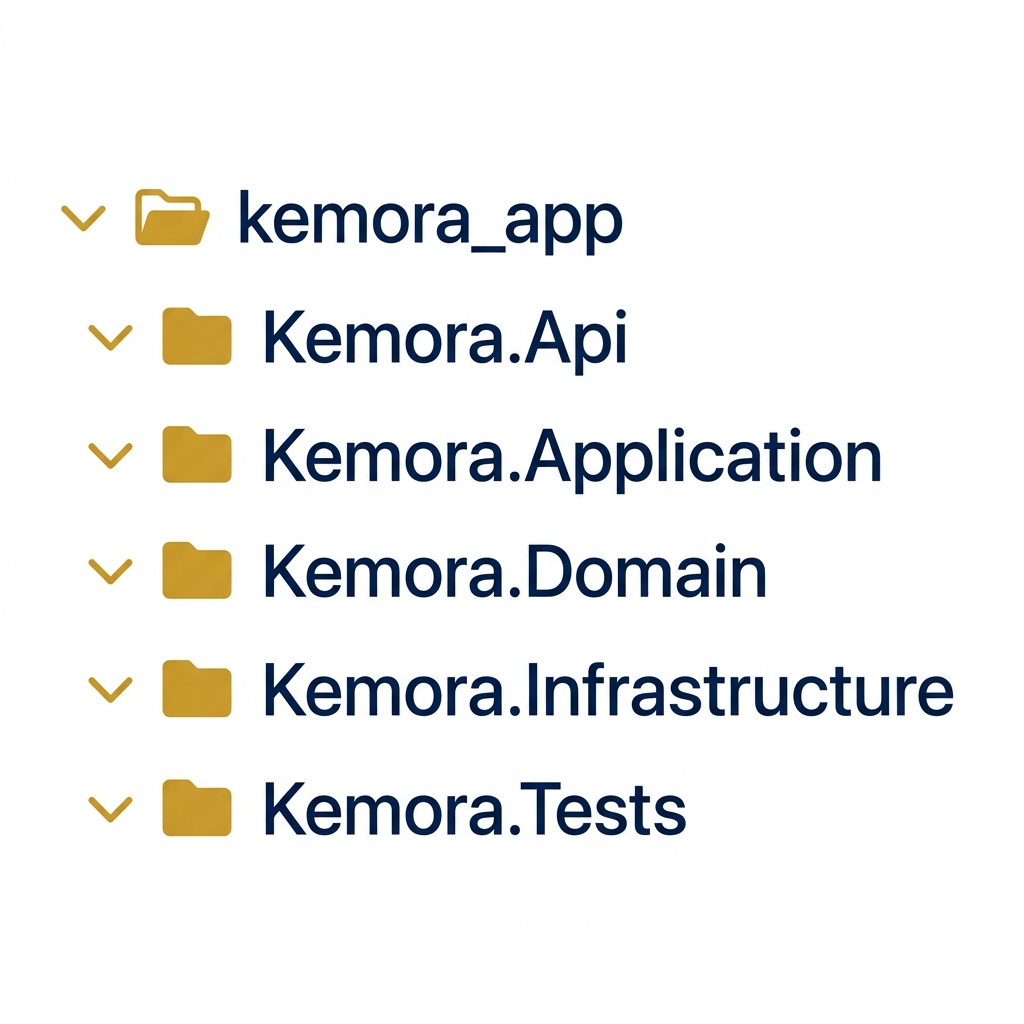
\includegraphics[width=0.9\textwidth]{figures/architecture.png}
    \caption{Kemora's Overall Architecture}
    \label{fig:architecture}
\end{figure}

\subsection{Sequence Diagrams}

\subsubsection{Authentication Flow (JWT Generation)}
The following Mermaid sequence diagram illustrates the login and token generation process when a user authenticates via the \texttt{AuthController}.

\begin{verbatim}
sequenceDiagram
    participant Client as Flutter App
    participant API as AuthController
    participant AuthSvc as AuthService
    participant SignIn as SignInManager
    participant Identity as UserManager
    participant TokenSvc as TokenService
    participant DB as SQL Server

    Client->>API: POST /api/v1/auth/login (email, password)
    API->>AuthSvc: LoginAsync(model)
    AuthSvc->>Identity: FindByEmailAsync(email)
    Identity->>DB: Query User
    DB-->>Identity: Return ApplicationUser
    AuthSvc->>SignIn: CheckPasswordSignInAsync(user, password, false)
    SignIn-->>AuthSvc: Password Valid
    AuthSvc->>TokenSvc: GenerateRefreshToken()
    TokenSvc-->>AuthSvc: Return 32-byte Base64 String
    AuthSvc->>Identity: UpdateAsync(user)
    Identity->>DB: Save Refresh Token to User
    AuthSvc->>TokenSvc: CreateTokenAsync(user)
    TokenSvc->>Identity: GetRolesAsync(user)
    Identity-->>TokenSvc: List of Roles
    Note over TokenSvc: Sign JWT & Attach Claims
    TokenSvc-->>AuthSvc: Return JWT String
    AuthSvc-->>API: Return AuthResponseDto
    API-->>Client: 200 OK (Tokens + User Info)
\end{verbatim}

\subsubsection{AI Trip Generation \& Save Flow}
This diagram outlines the process of requesting an AI-generated itinerary and subsequently saving it to the database using the \texttt{PlacesController}, \texttt{TripsController}, and \texttt{OpenRouterAiService}.

\begin{verbatim}
sequenceDiagram
    participant Client as Flutter App
    participant PlacesAPI as PlacesController
    participant TripsAPI as TripsController
    participant PlannerSvc as TripPlannerService
    participant TripSvc as TripService
    participant AI as OpenRouterAiService
    participant ExtAI as OpenRouter API
    participant Badge as BadgeAwardService
    participant DB as SQL Server

    Client->>PlacesAPI: POST /api/v1/places/trip-plan (TripPlanRequestDto)
    PlacesAPI->>PlannerSvc: GenerateTripPlanAsync(request)
    PlannerSvc->>AI: GenerateCompletionAsync(sysPrompt, userPrompt)
    Note over AI: Check ConcurrentDictionary<br/>for available free models
    AI->>ExtAI: HTTP POST /v1/completions
    ExtAI-->>AI: LLM JSON Response (Itinerary)
    AI-->>PlannerSvc: Parsed TripPlanResponseDto
    PlannerSvc-->>PlacesAPI: Return TripPlanResponseDto
    PlacesAPI-->>Client: 200 OK (Proposed Itinerary)
    
    Note over Client: User reviews and modifies<br/>the itinerary locally
    
    Client->>TripsAPI: POST /api/v1/trips/save-plan (SaveAIPlanDto)
    TripsAPI->>TripSvc: SaveAIPlanAsync(userId, dto)
    TripSvc->>DB: Insert Trip & TripPlaces
    DB-->>TripSvc: Assigned TripID
    TripSvc-->>TripsAPI: Return TripDetailDto
    
    TripsAPI->>Badge: TryAwardAiPioneerAsync(userId)
    Badge->>DB: Check/Update User Badges
    TripsAPI->>Badge: TryAwardCityHopperAsync(userId)
    TripsAPI-->>Client: 201 Created (Trip details)
\end{verbatim}

\subsection{Microservices Readiness \& Bounded Contexts}
Although Kemora is currently deployed as a modular monolith to reduce operational overhead, its architecture is fundamentally designed for a seamless transition to microservices. By strictly adhering to Clean Architecture \cite{cleanarchitecture} and employing MediatR \cite{mediatr} for domain events, the system establishes clear bounded contexts (e.g., Identity, Trip Planning, Social Feed, Gamification). These bounded contexts interact through asynchronous events rather than direct method calls. When the platform scales to a point where independent deployment of these domains becomes necessary, the in-memory MediatR pipelines can easily be replaced with distributed event brokers, such as RabbitMQ \cite{rabbitmq} or Apache Kafka \cite{kafka}, with minimal refactoring of the core business logic.

\section{Database Design and Entity Relationships}
The data tier is powered by a relational SQL Server database schema optimized for entity integrity and rapid querying. The schema is managed via Entity Framework Core \cite{efcore} Code-First migrations.

\subsection{Key Data Entities}
\begin{itemize}
    \item \textbf{ApplicationUser:} Inherits from ASP.NET Identity User. Holds authentication details, accumulated points, and JSON-serialized user preferences.
    \item \textbf{Place \& Governorate:} Hierarchical spatial data. Places are linked to Governorates via foreign keys and are categorized by \texttt{PlaceType}.
    \item \textbf{Trip \& TripPlace:} Represents the AI-generated itineraries. A \texttt{Trip} has a one-to-many relationship with \texttt{TripPlace}, representing the chronological ordering of activities (with precise \texttt{Order} fields for timeline mapping).
    \item \textbf{Post \& Comment:} The core of the social network. Posts link to a \texttt{UserID} and optionally a \texttt{LinkedTripId}, allowing users to seamlessly share their itineraries directly to the feed.
\end{itemize}

\begin{figure}[H]
    \centering
    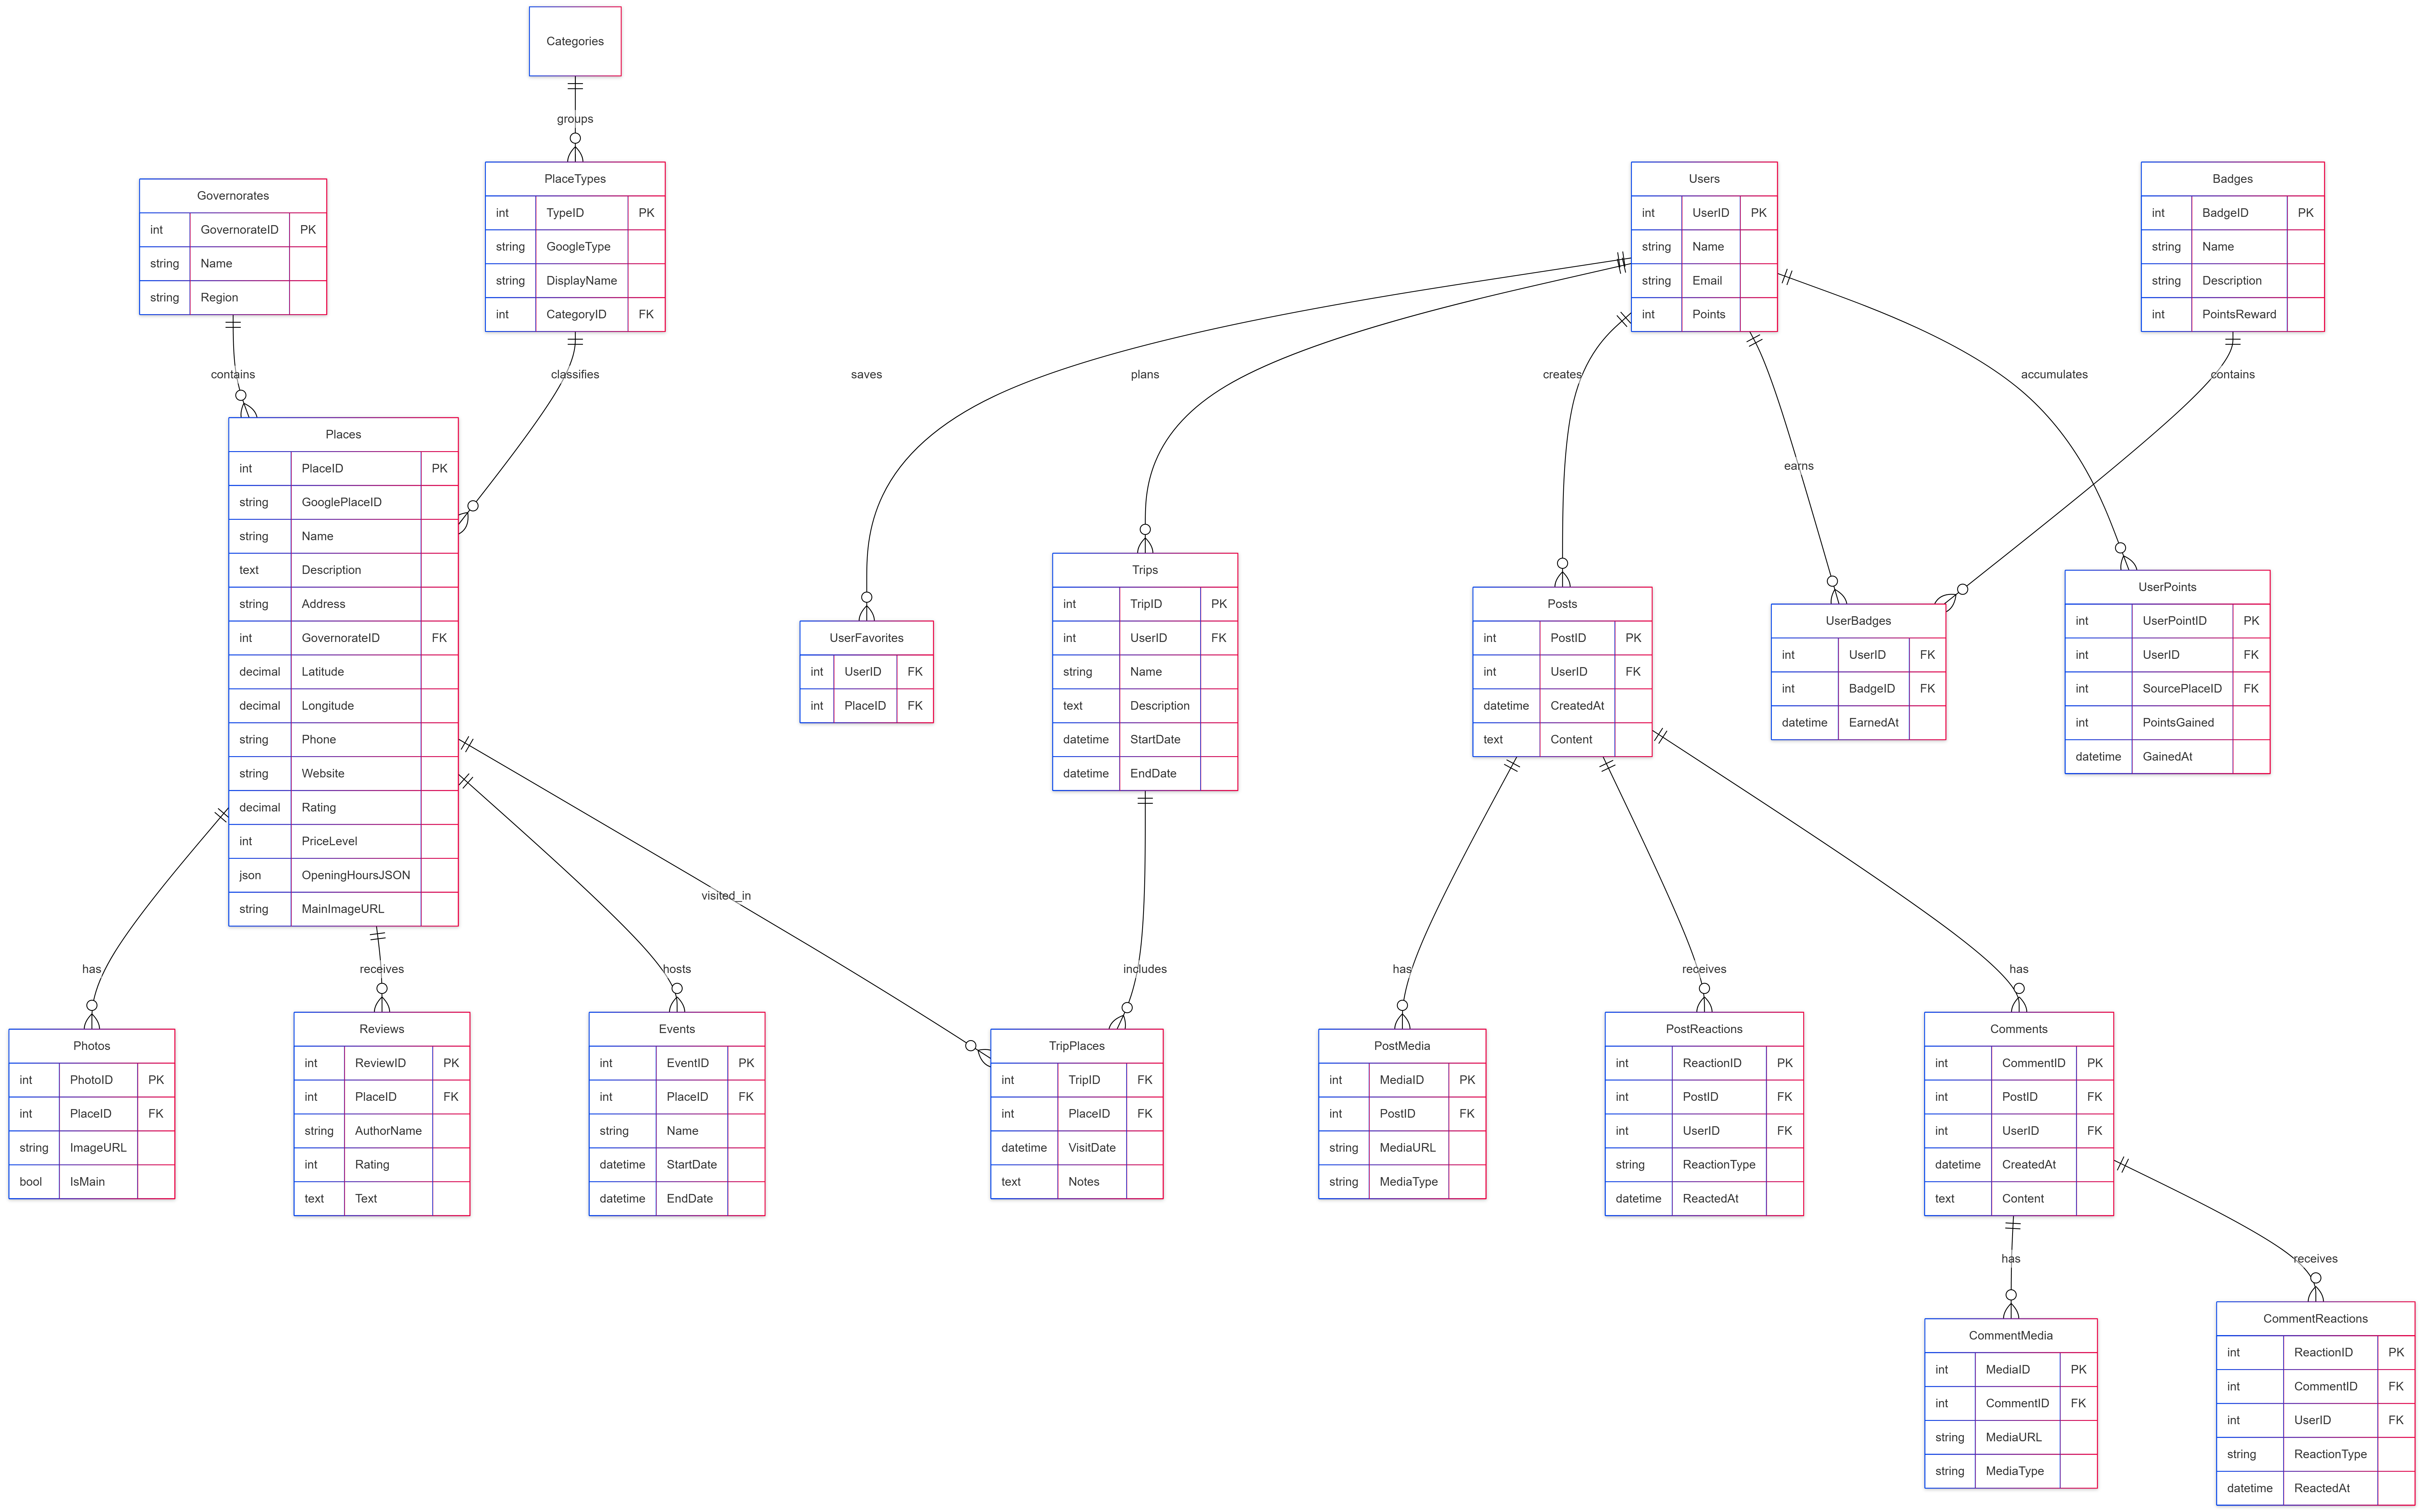
\includegraphics[width=0.9\textwidth]{figures/erd.png}
    \caption{Entity Relationship Diagram (ERD)}
    \label{fig:erd}

\end{figure}

\section{Frontend Architecture \& State Management Journey}
Building a visually rich, heavily interactive frontend for Kemora posed a significant challenge: State Management. Initially, passing state down the widget tree via constructors led to "prop drilling," making the UI rigid and difficult to test. 

To conquer this, we adopted the \textbf{Provider} pattern \cite{providerpattern}. Provider allowed us to cleanly separate our UI rendering from our business logic. By injecting ViewModels and Services at the top of the tree, any widget could reactively listen to state changes without tightly coupling to the data source. This decision transformed our Flutter application (\texttt{lib/presentation/}) into a highly modular, testable, and responsive frontend. The User Interface (UI) follows a "Modern Heritage" design language—blending contemporary mobile UX patterns (glassmorphism, vibrant gradients) with culturally resonant typography and color palettes.

Beyond state management, a robust \textbf{Mobile Security \& Offline Data Strategy} is implemented to ensure data integrity and user privacy. Sensitive credentials, such as JWTs and refresh tokens, are securely persisted using \textbf{Flutter Secure Storage}, leveraging native platform keystores. For performance and offline capabilities, frequently accessed data and user preferences are cached locally using high-performance embedded databases like \textbf{SQLite} and \textbf{Hive}, minimizing network overhead and allowing the application to gracefully handle intermittent connectivity.

\subsection{Journey 1: Onboarding \& Authentication}
The user is first greeted by an animated Splash Screen, followed by an educational Walkthrough. The Authentication flow supports standard registration and OAuth. It intercepts deep links for email confirmation and password resets.

\begin{figure}[H]
    \centering
    \begin{minipage}[t]{0.45\textwidth}
        \centering
        \vspace{0pt}
        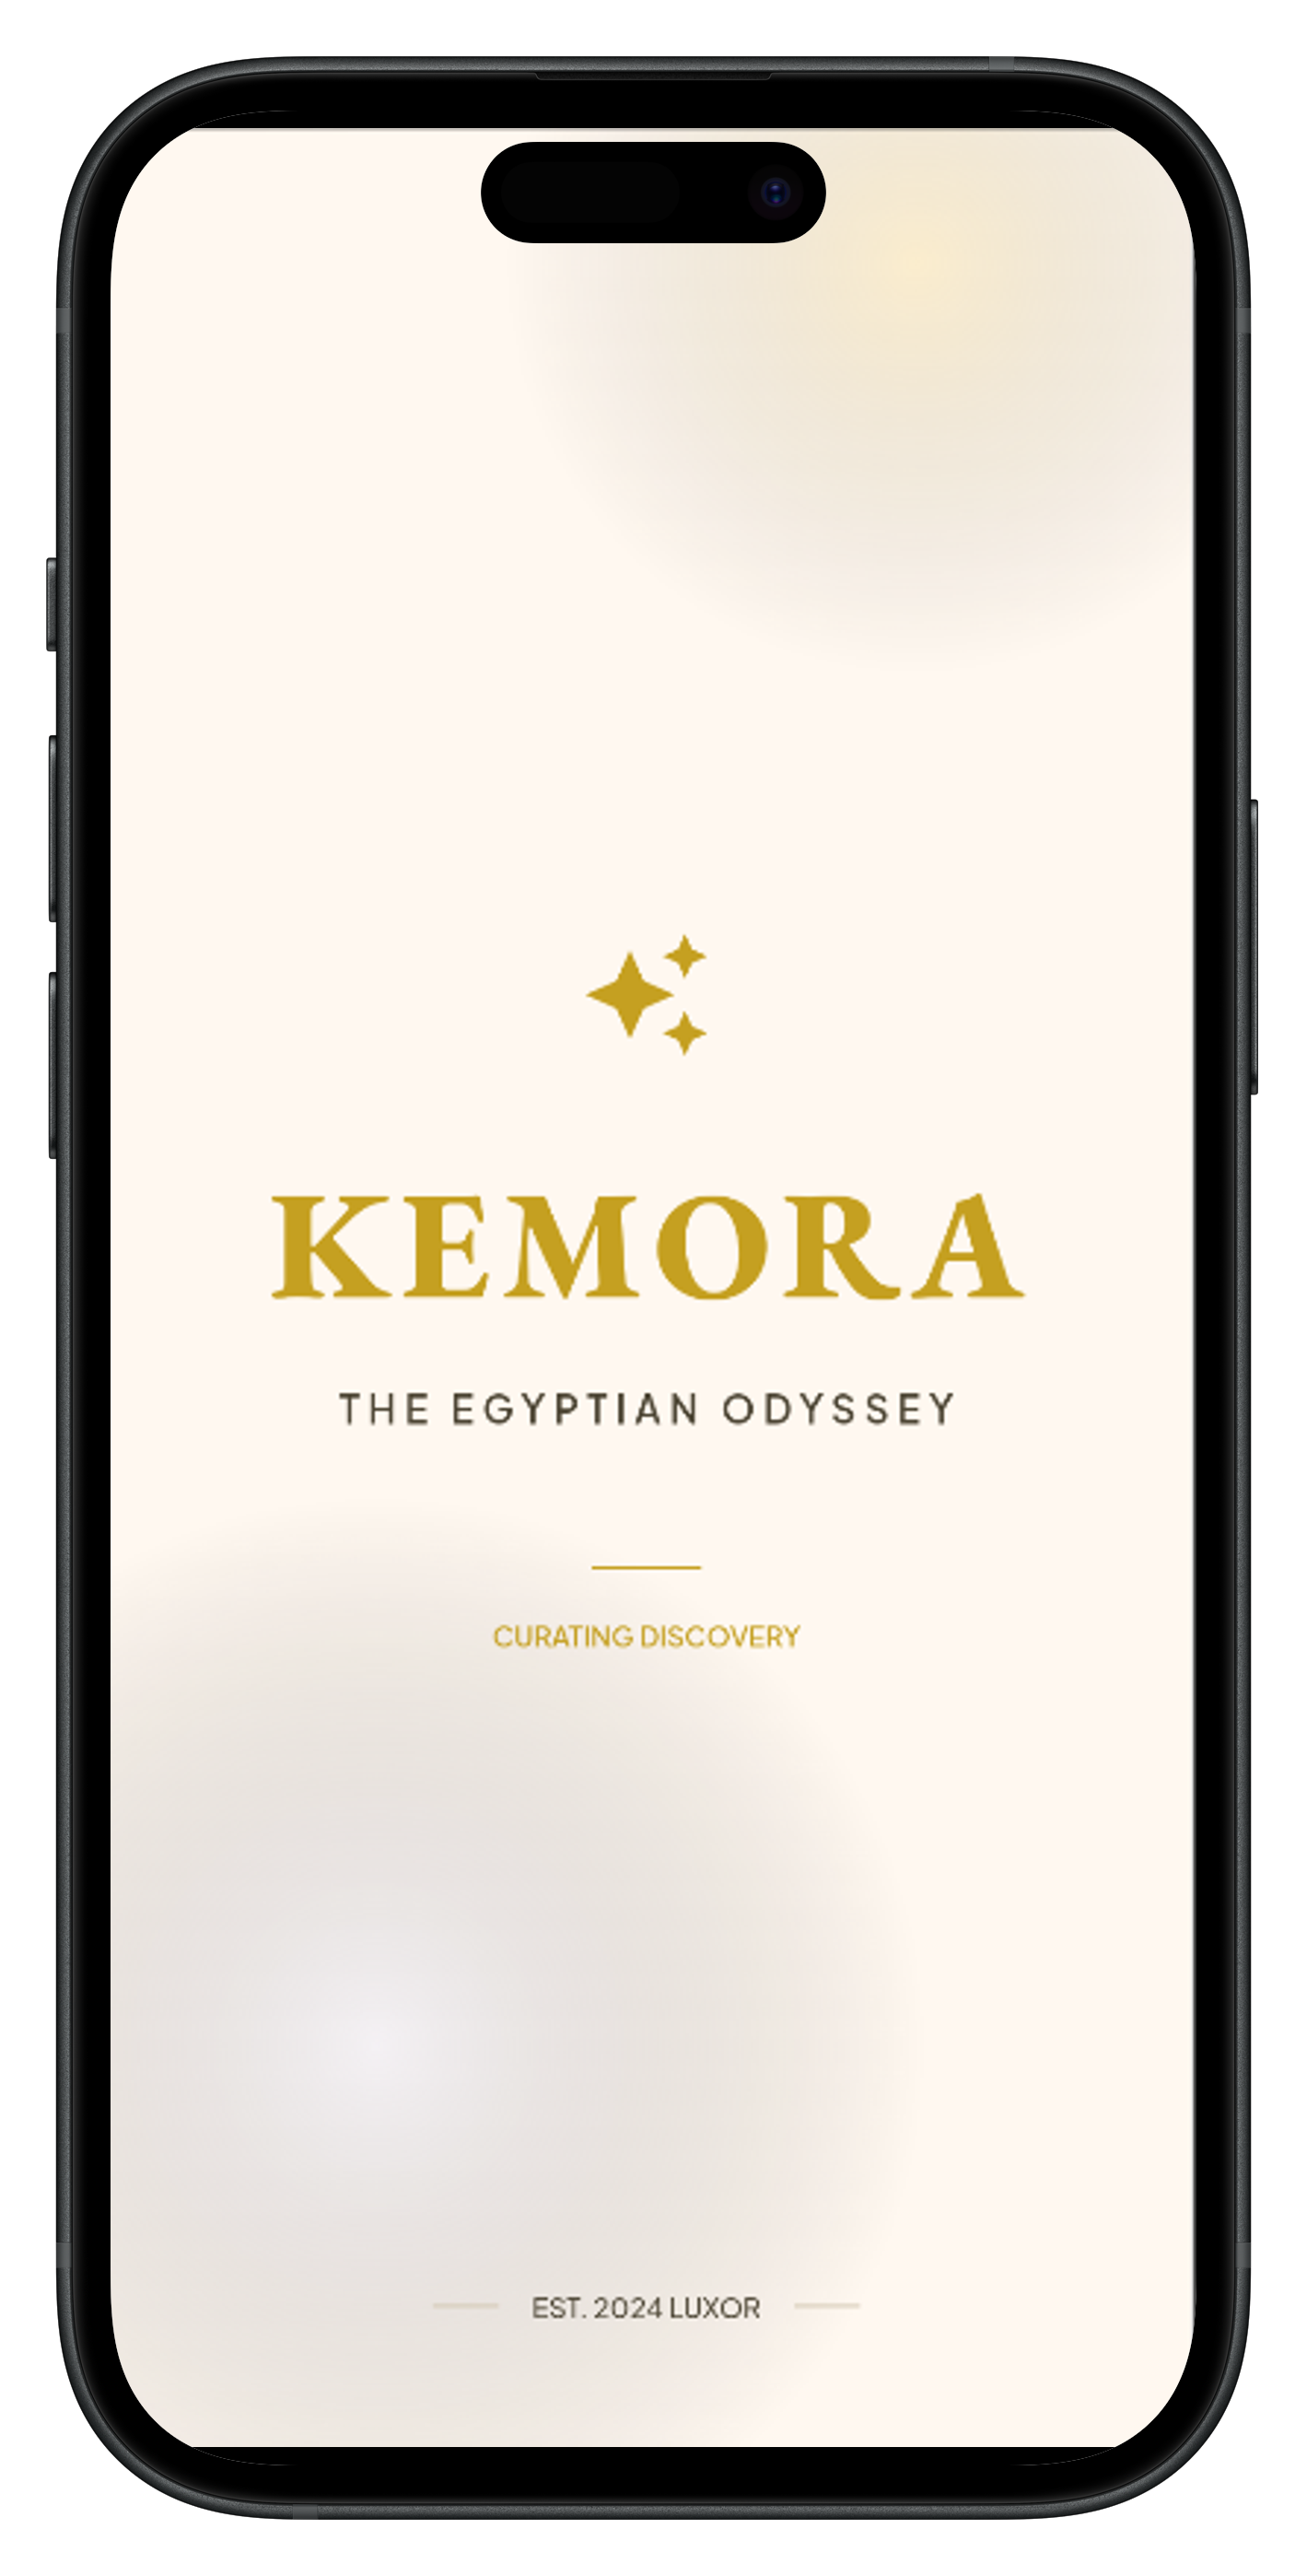
\includegraphics[width=\linewidth]{figures/splash.png}
        \caption{Mobile Application Splash Screen}
        \label{fig:splash}
    \end{minipage}\hfill
    \begin{minipage}[t]{0.45\textwidth}
        \centering
        \vspace{0pt}
        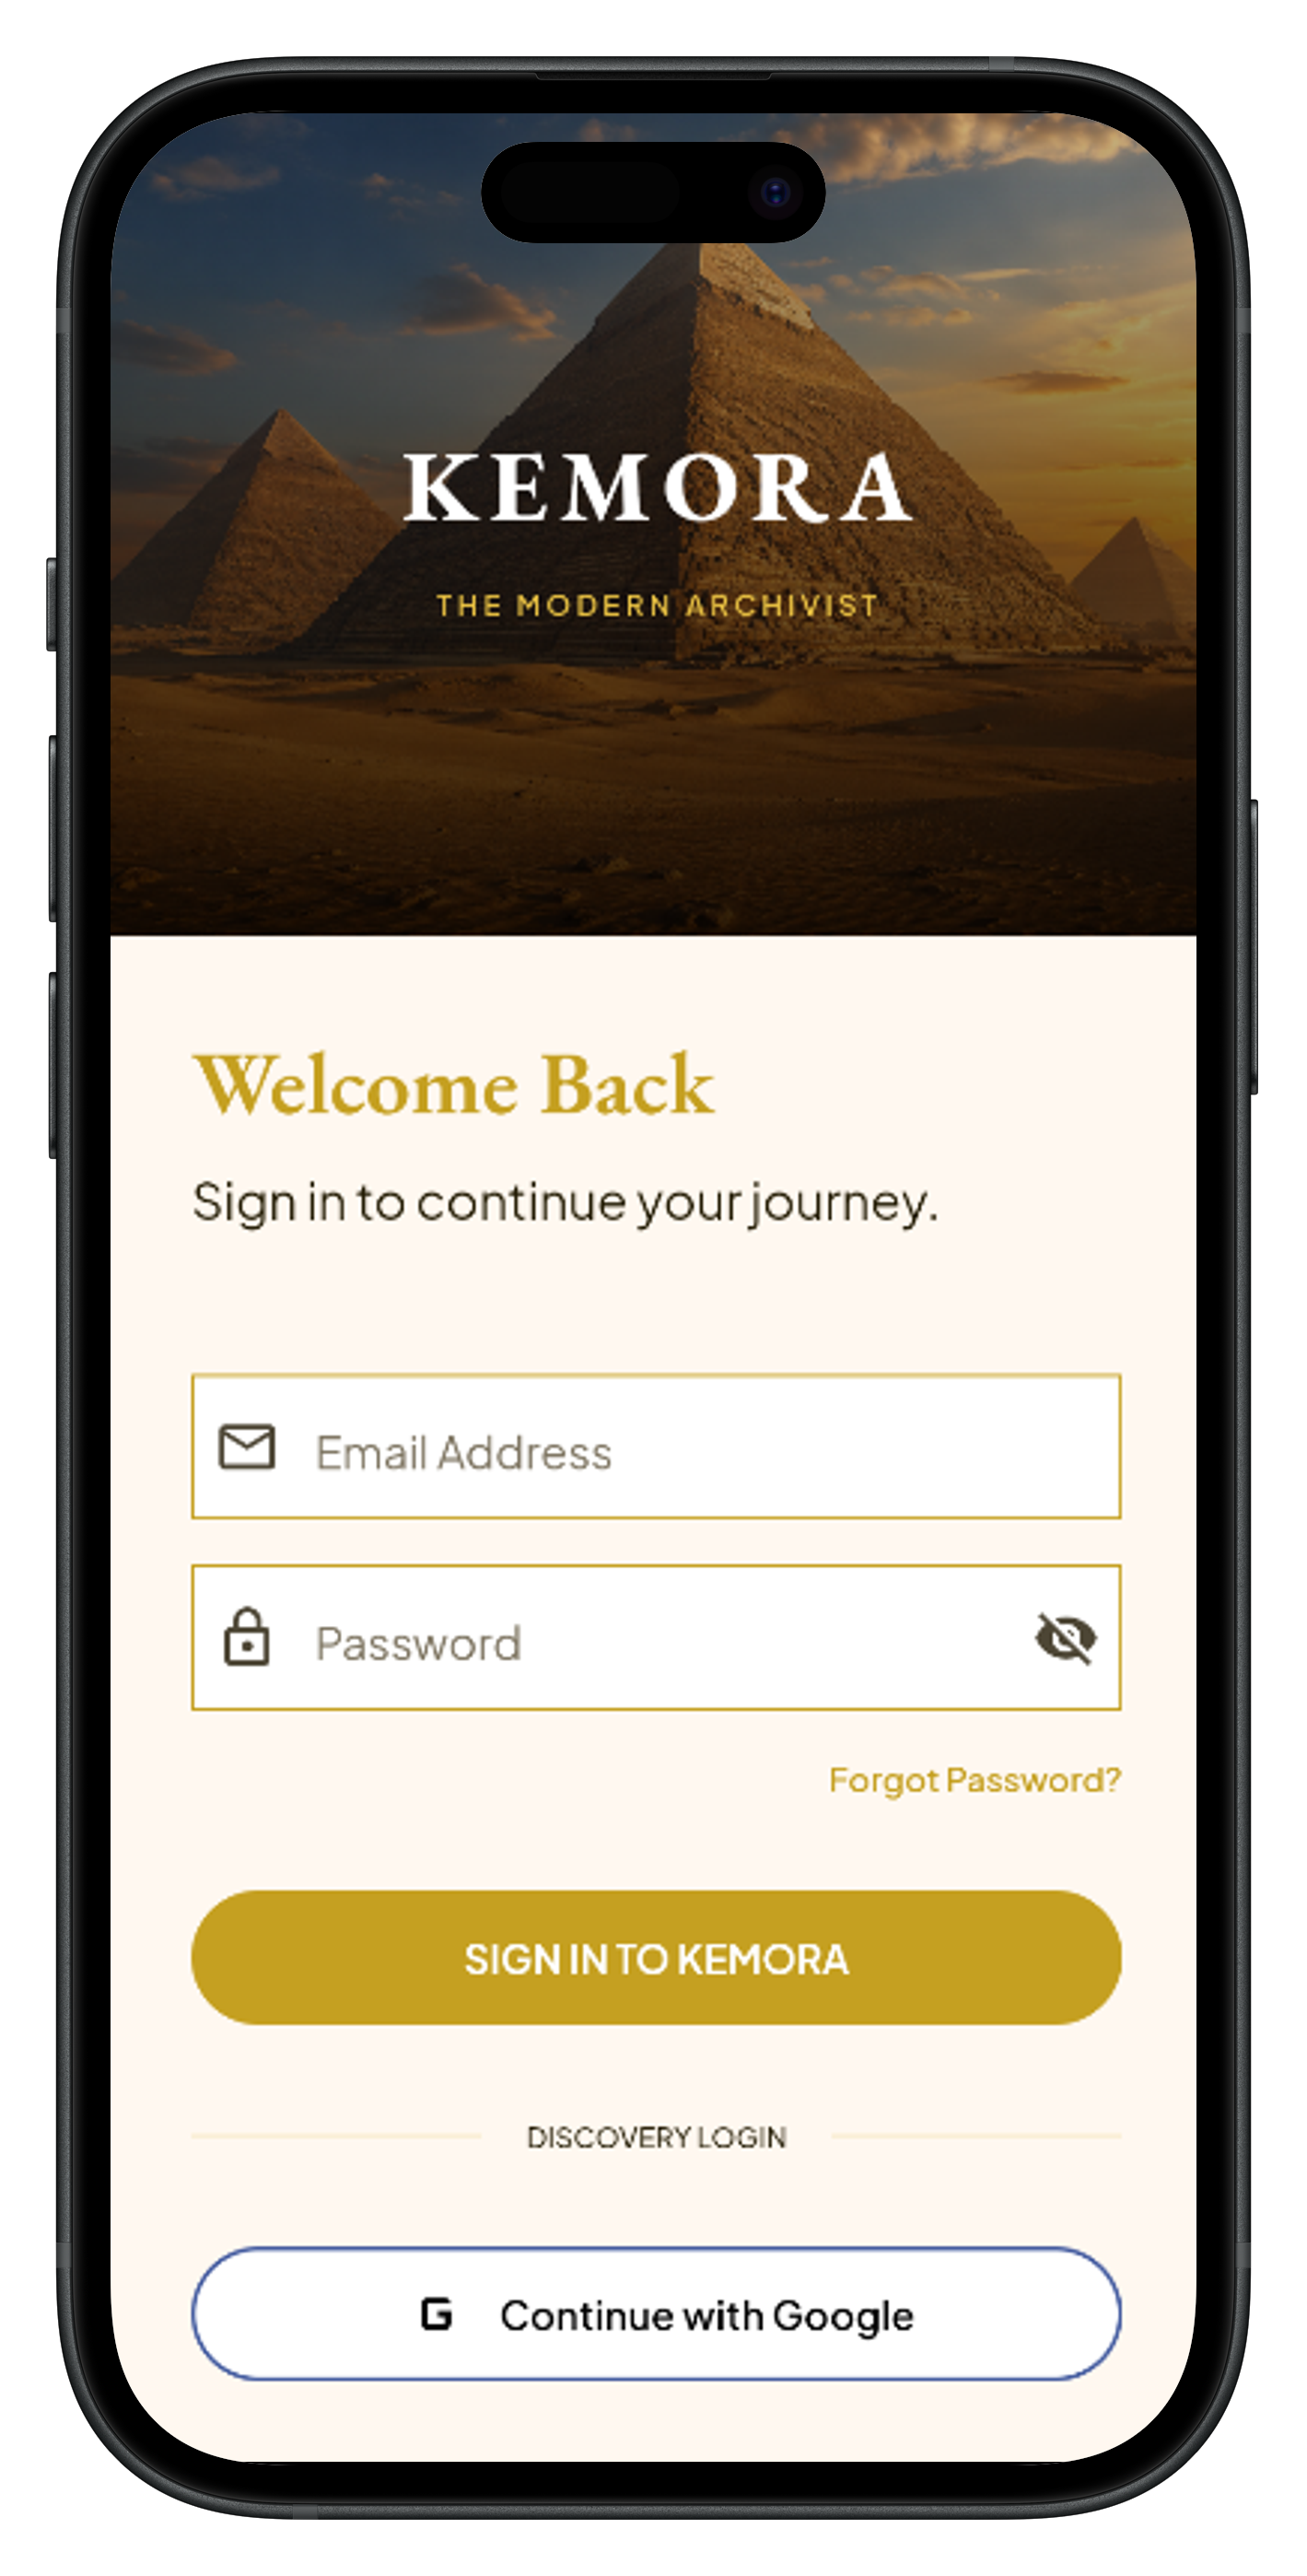
\includegraphics[width=\linewidth]{figures/login.png}
        \caption{Mobile Application Authentication Page}
        \label{fig:login}
    \end{minipage}
\end{figure}

\subsection{Journey 2: Main Dashboard \& Discovery}
The Home screen serves as the central hub, presenting personalized recommendations, top-rated destinations, and quick-action navigation via a custom floating tab bar.

\begin{figure}[H]
    \centering
    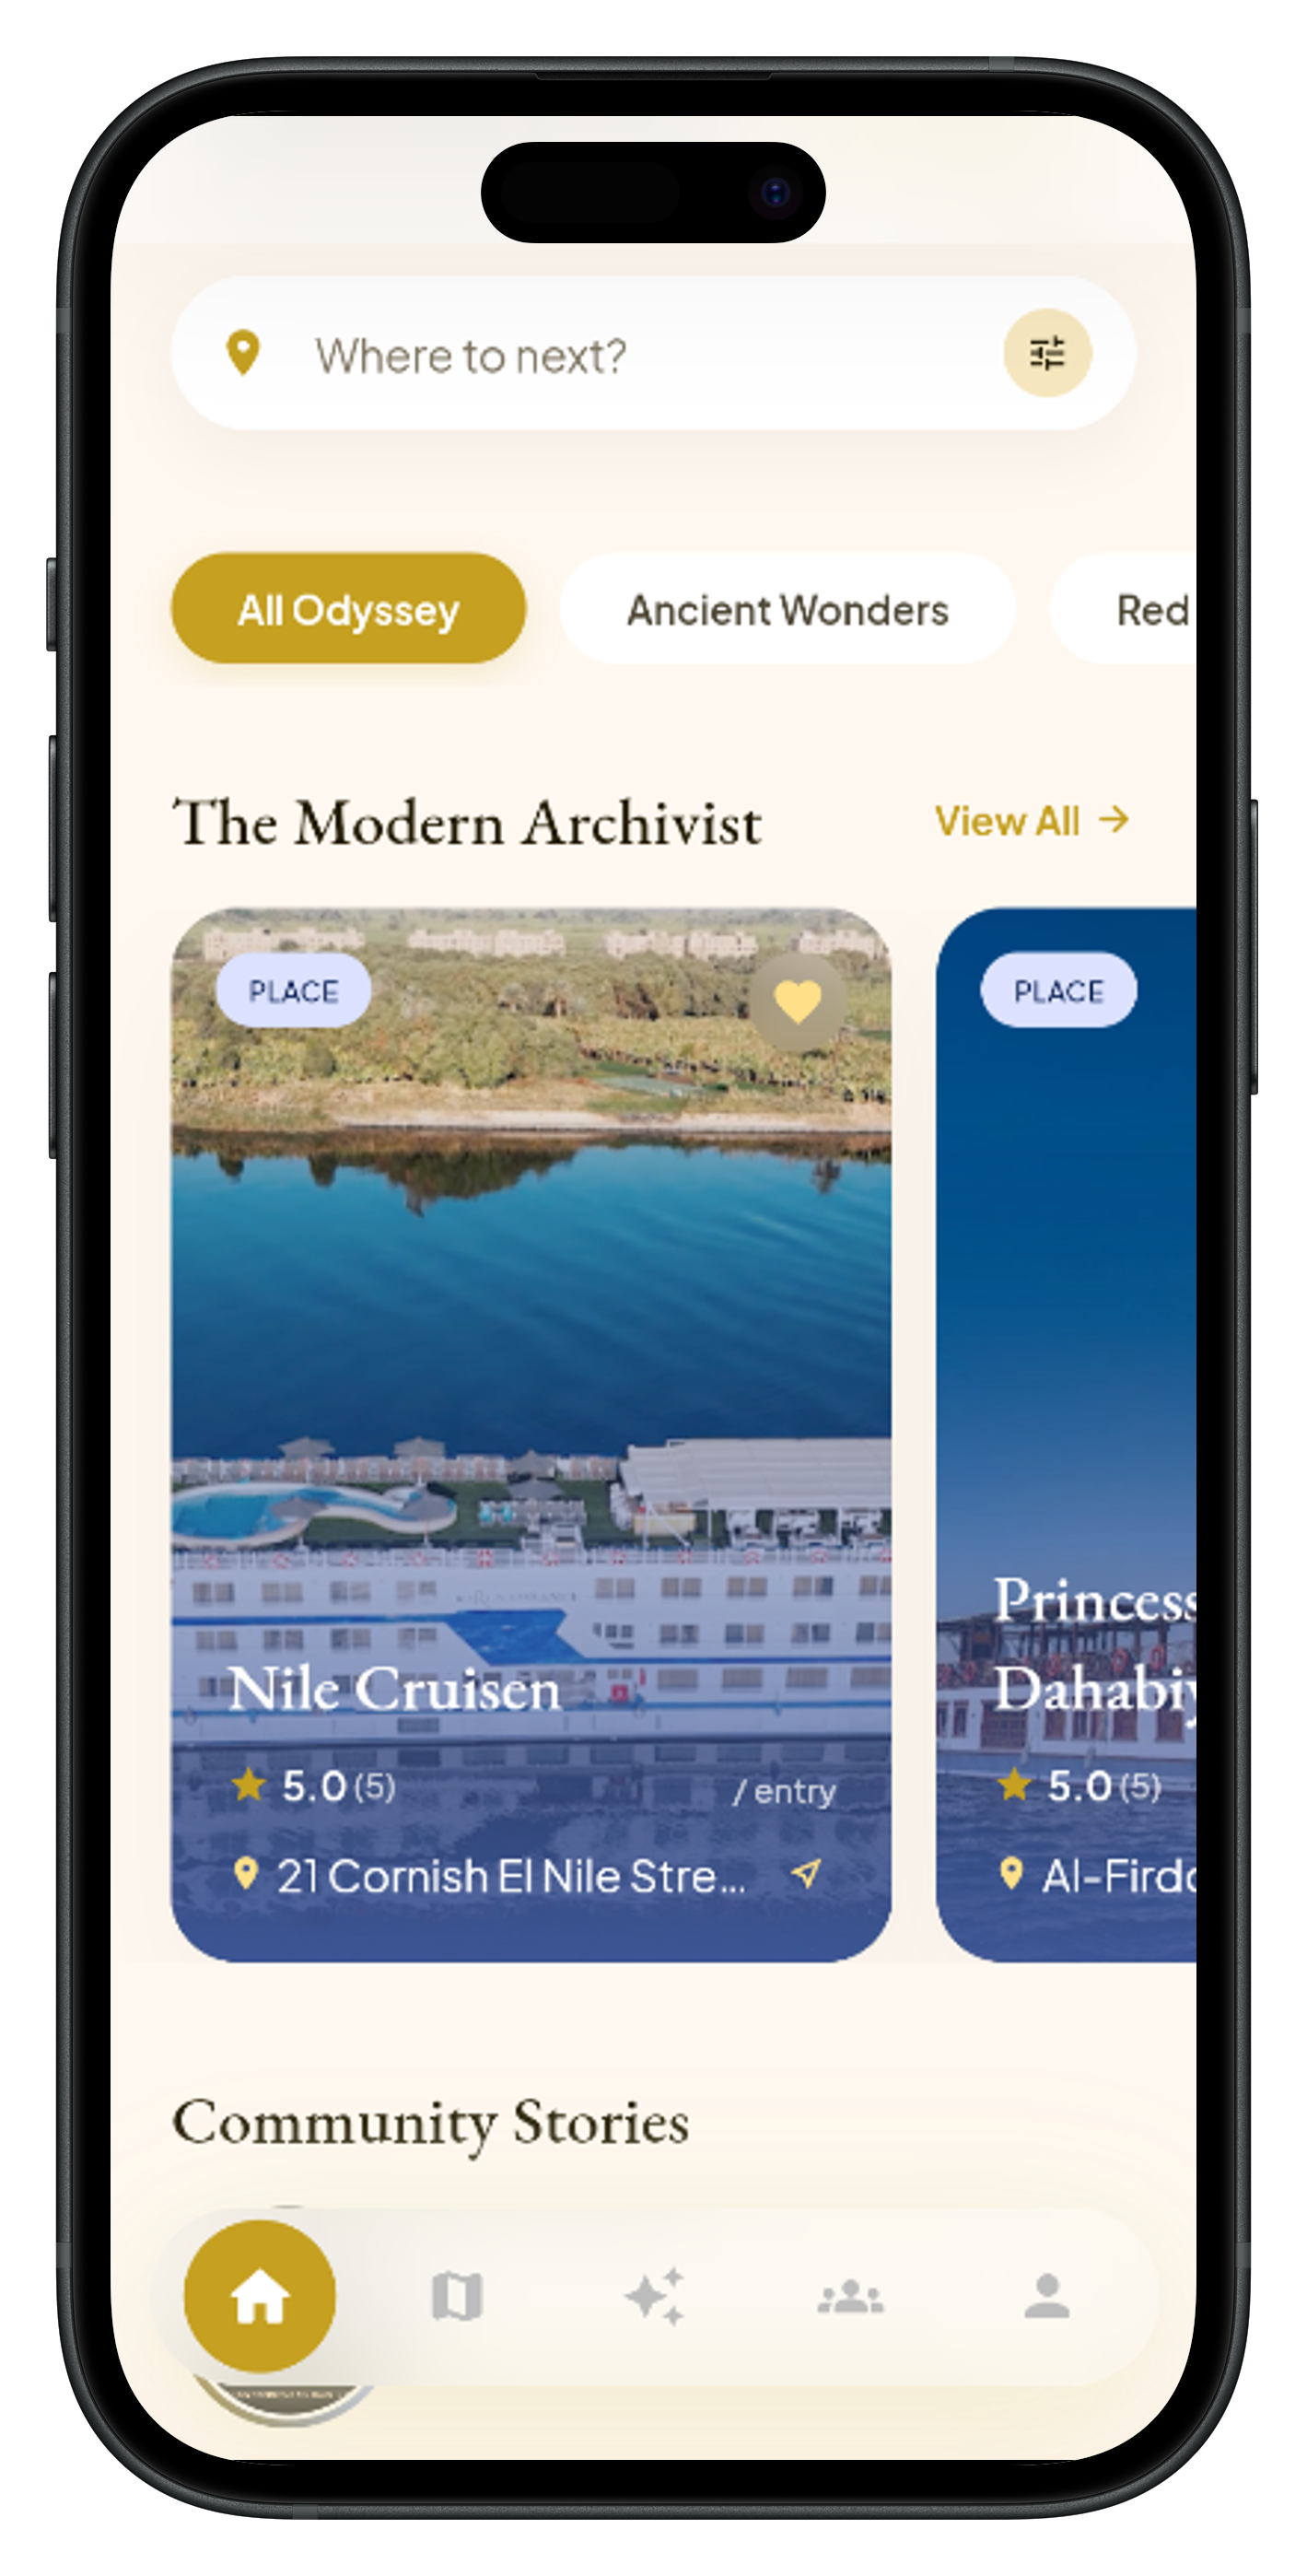
\includegraphics[width=0.45\textwidth]{figures/home.png}
    \caption{Mobile Application Home Page}
    \label{fig:home}
\end{figure}

\subsection{Journey 3: Explore \& Location Discovery}
Users can navigate an interactive map of Egyptian governorates. Selecting a governorate transitions to a detailed view listing sub-categories (Historical, Coastal, etc.) and individual Place detail screens.

\begin{figure}[H]
    \centering
    \begin{minipage}[t]{0.45\textwidth}
        \centering
        \vspace{0pt}
        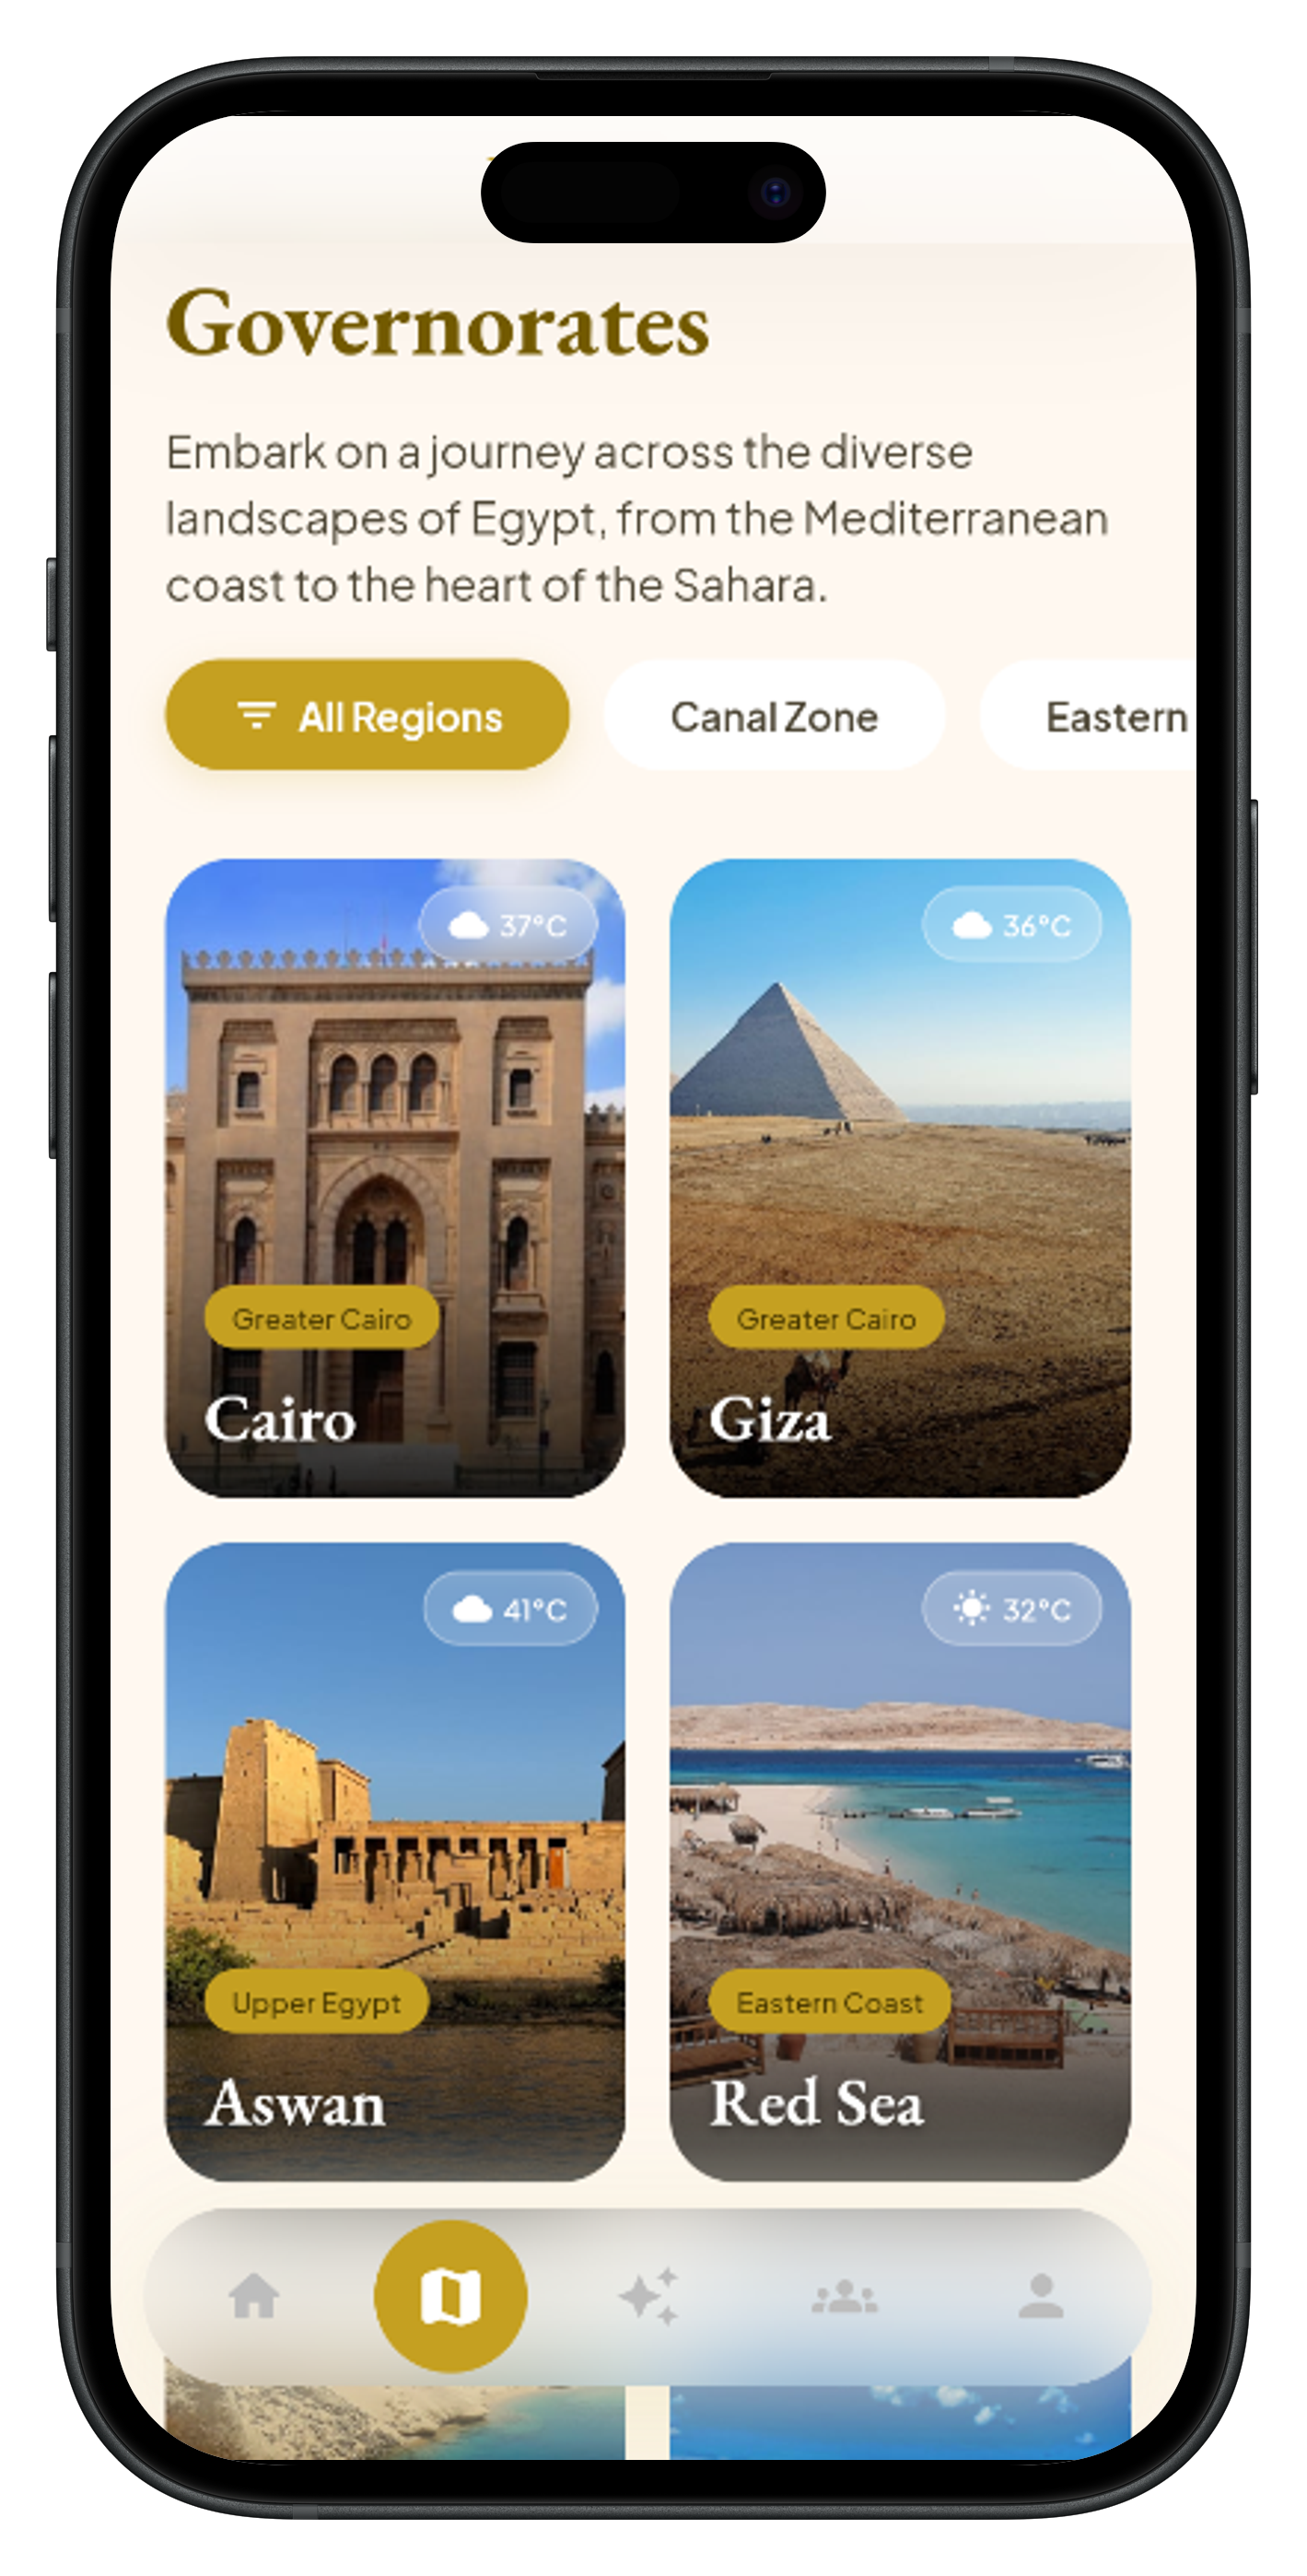
\includegraphics[width=\linewidth]{figures/gov_details.png}
        \caption{Governorate Details}
        \label{fig:gov_details}
    \end{minipage}\hfill
    \begin{minipage}[t]{0.45\textwidth}
        \centering
        \vspace{0pt}
        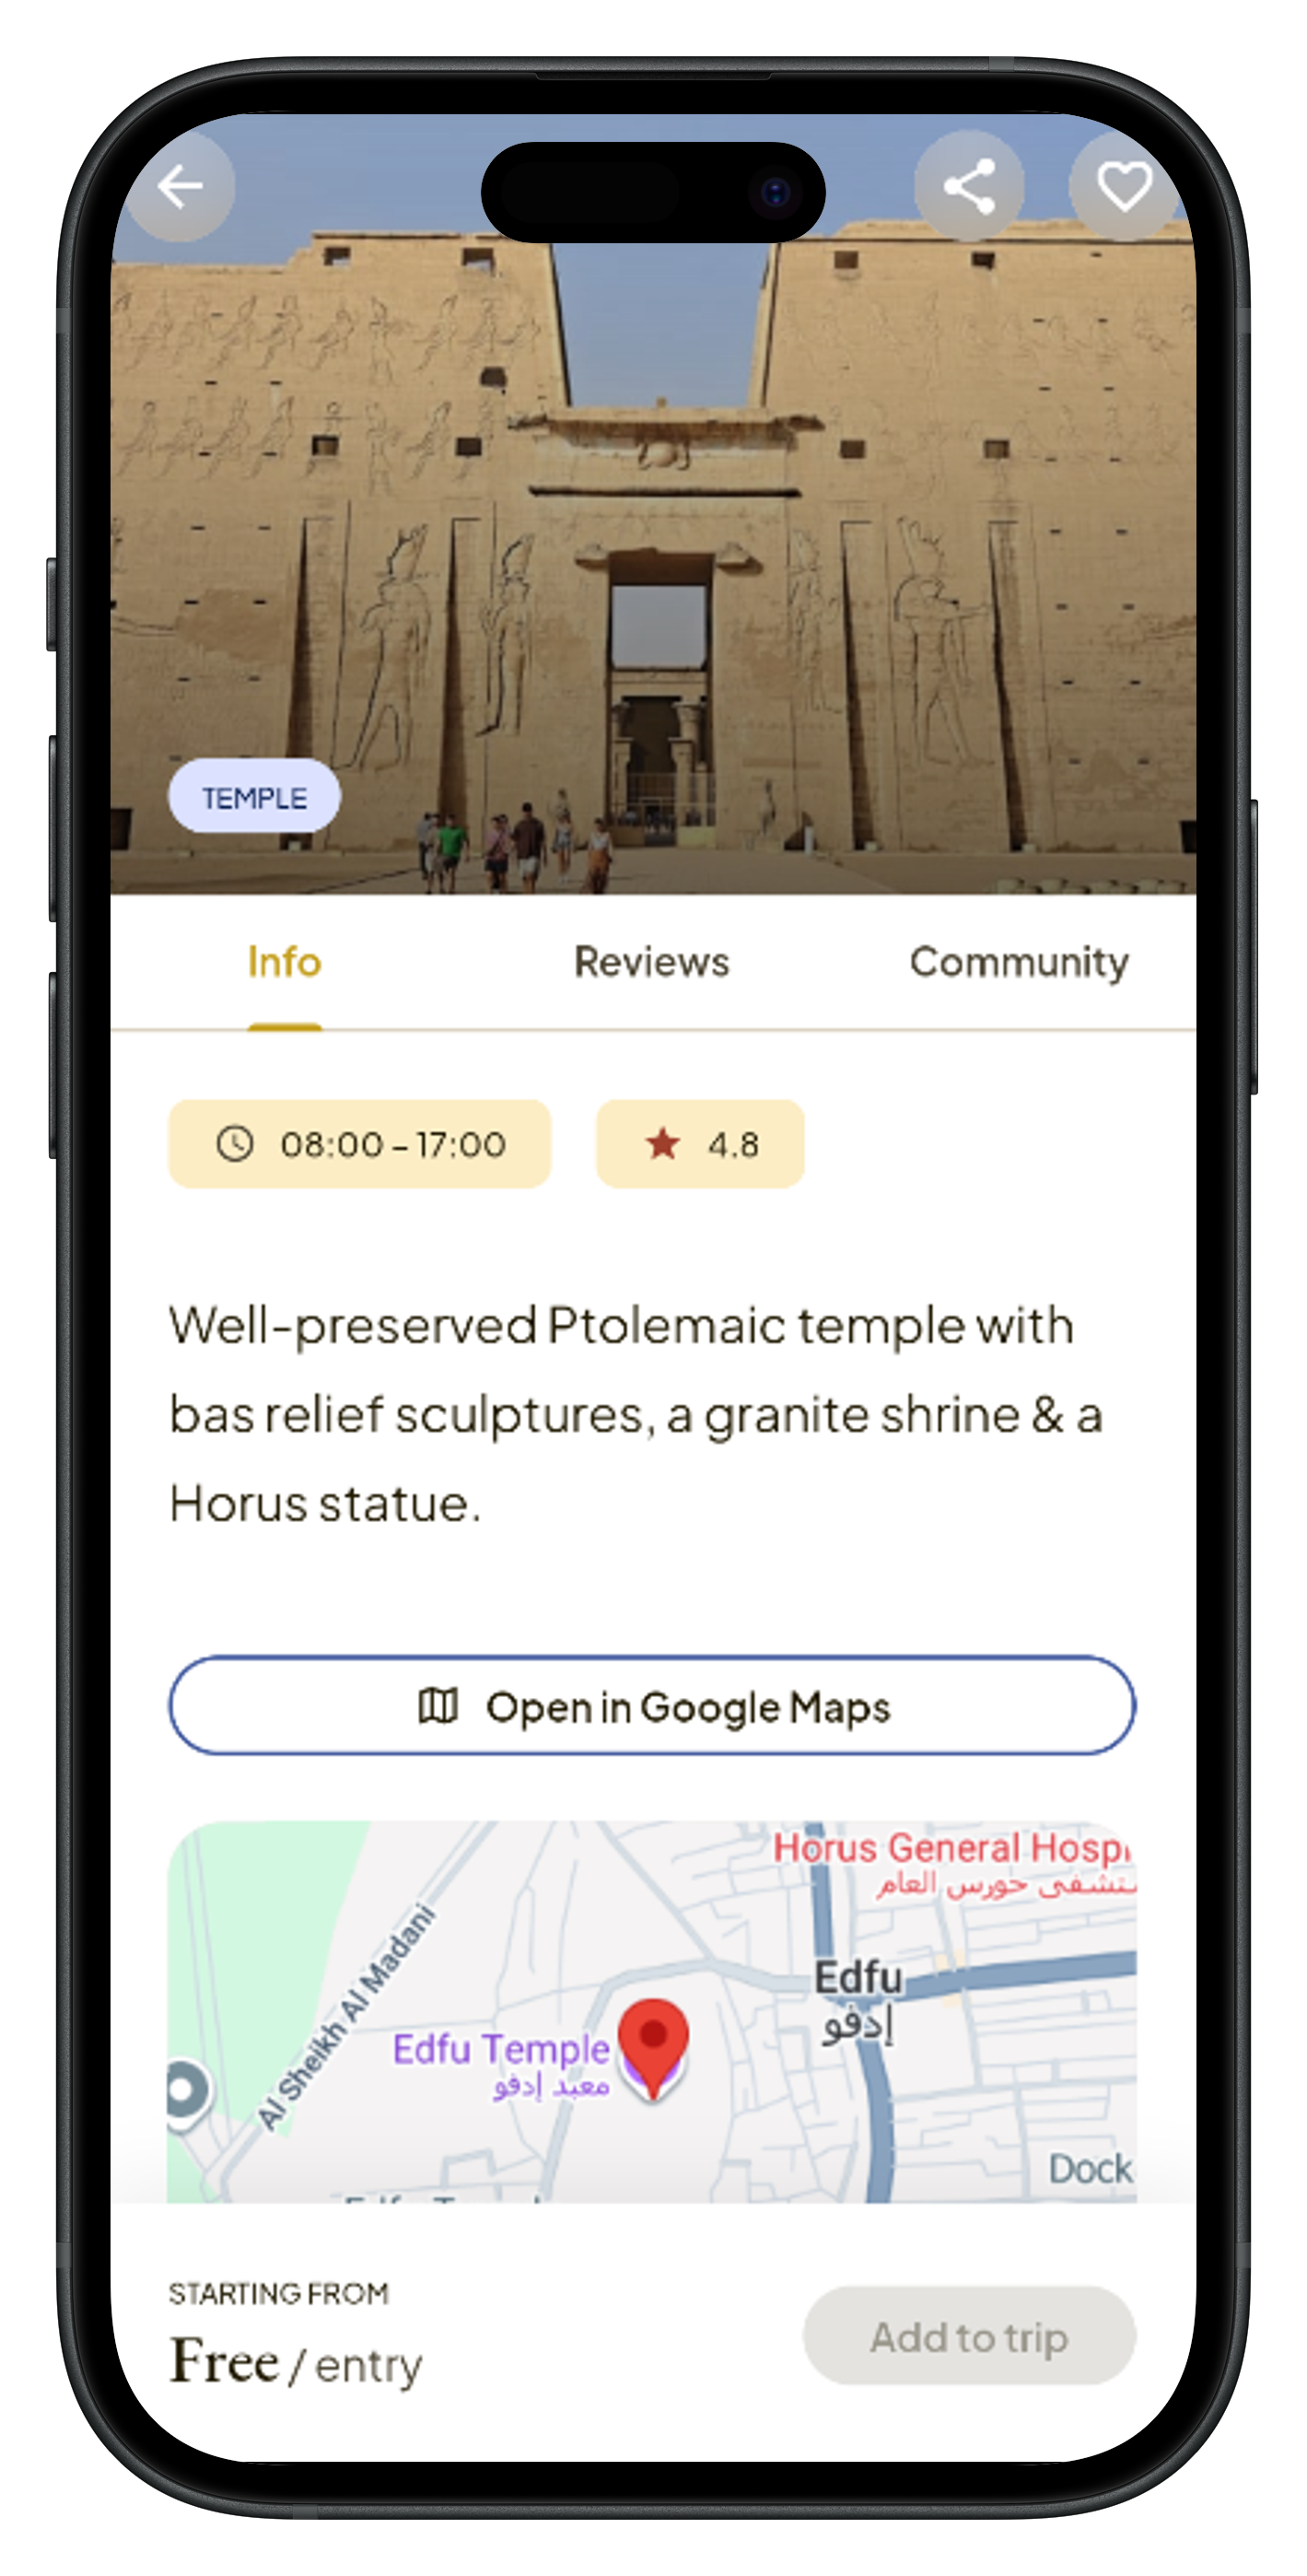
\includegraphics[width=\linewidth]{figures/place_details.png}
        \caption{Place Details}
        \label{fig:place_details}
    \end{minipage}
\end{figure}

\subsection{Journey 4: Trip Planning \& AI Itinerary}
This is the flagship journey. Users input parameters into a multi-step questionnaire (\texttt{ai\_step\_questions\_screen.dart}). The system displays a loading animation while negotiating with the backend AI. The result is a beautifully rendered, interactive timeline (\texttt{ai\_itinerary\_result\_screen.dart}).

\begin{figure}[H]
    \centering
    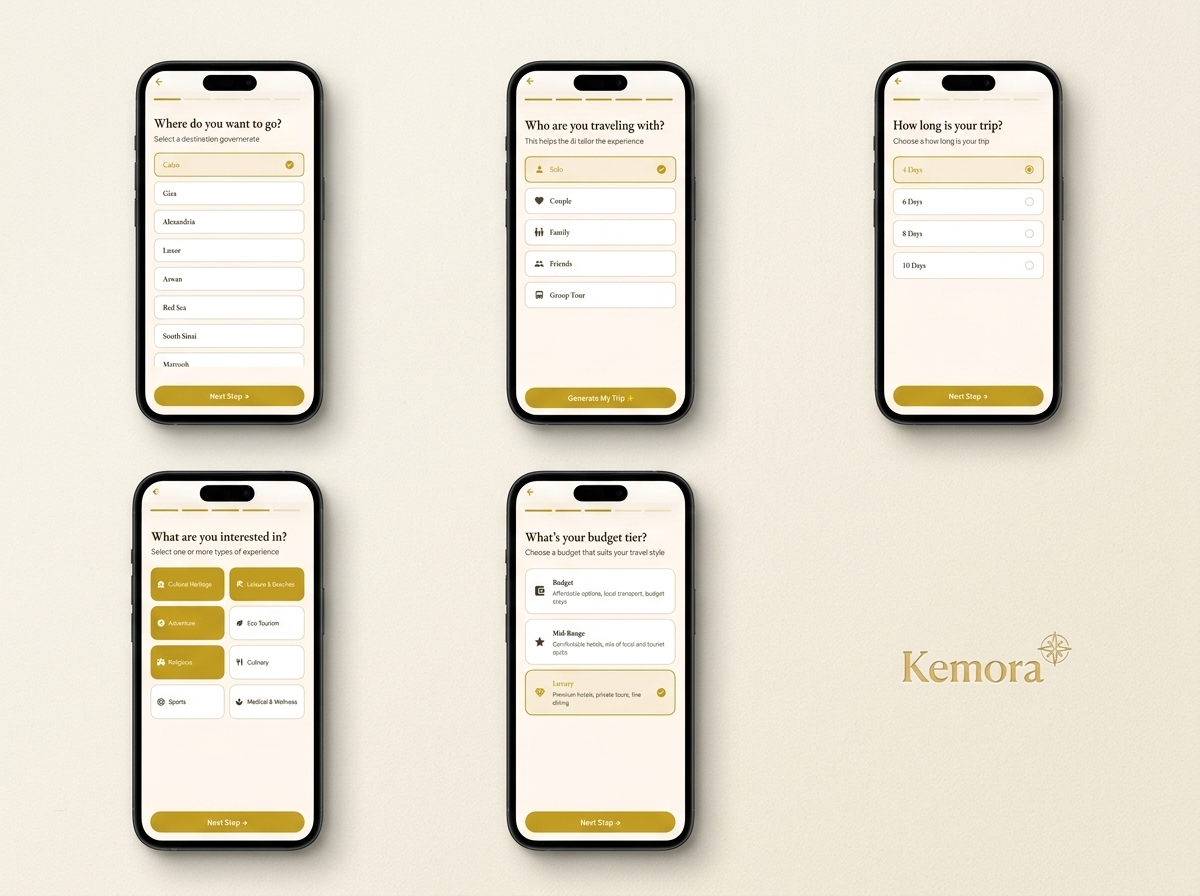
\includegraphics[width=\textwidth]{figures/ai_questions.png}
    \caption{AI Trip Planner Questionnaire}
    \label{fig:ai_questions}
\end{figure}

\subsection{Journey 5: Social \& Community}
A familiar, vertically scrolling feed allows users to consume and produce content. Users can view detailed posts and engage in comment threads.

\begin{figure}[H]
    \centering
    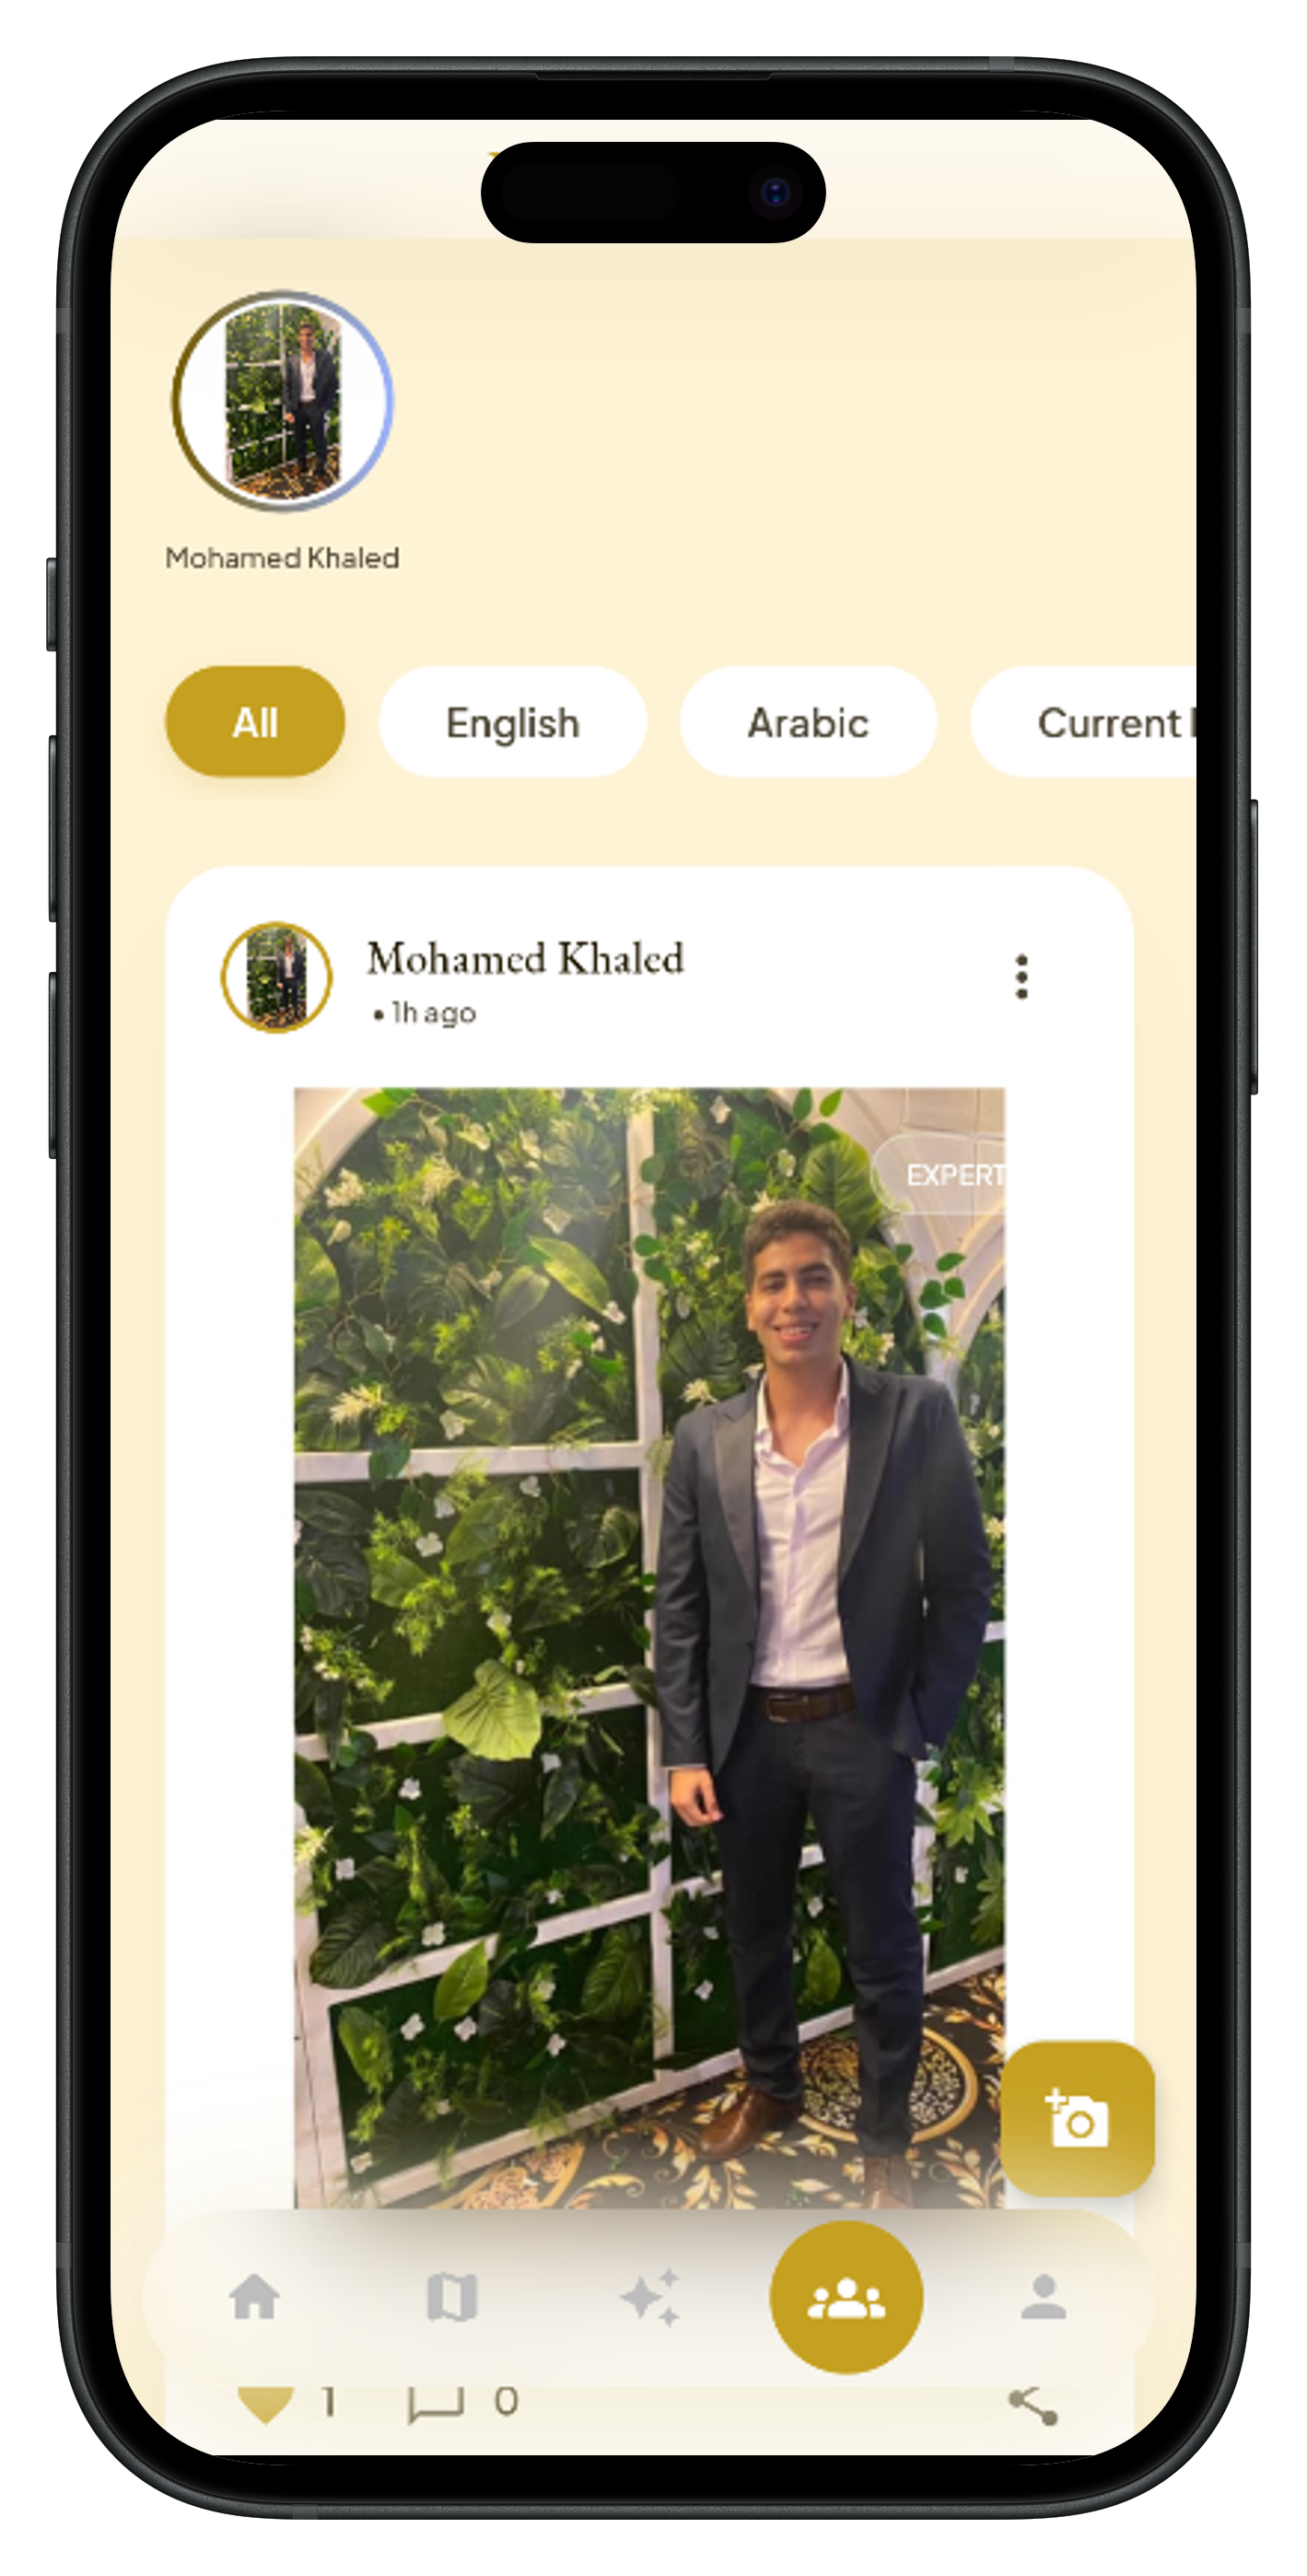
\includegraphics[width=0.45\textwidth]{figures/social_feed.png}
    \caption{Community Social Feed}
    \label{fig:social_feed}
\end{figure}

\subsection{Journey 6: Profile \& Gamification}
The Profile screen tracks the user's identity, displaying earned badges, total points, redeemed vouchers, and saved places.

\begin{figure}[H]
    \centering
    \begin{minipage}[t]{0.45\textwidth}
        \centering
        \vspace{0pt}
        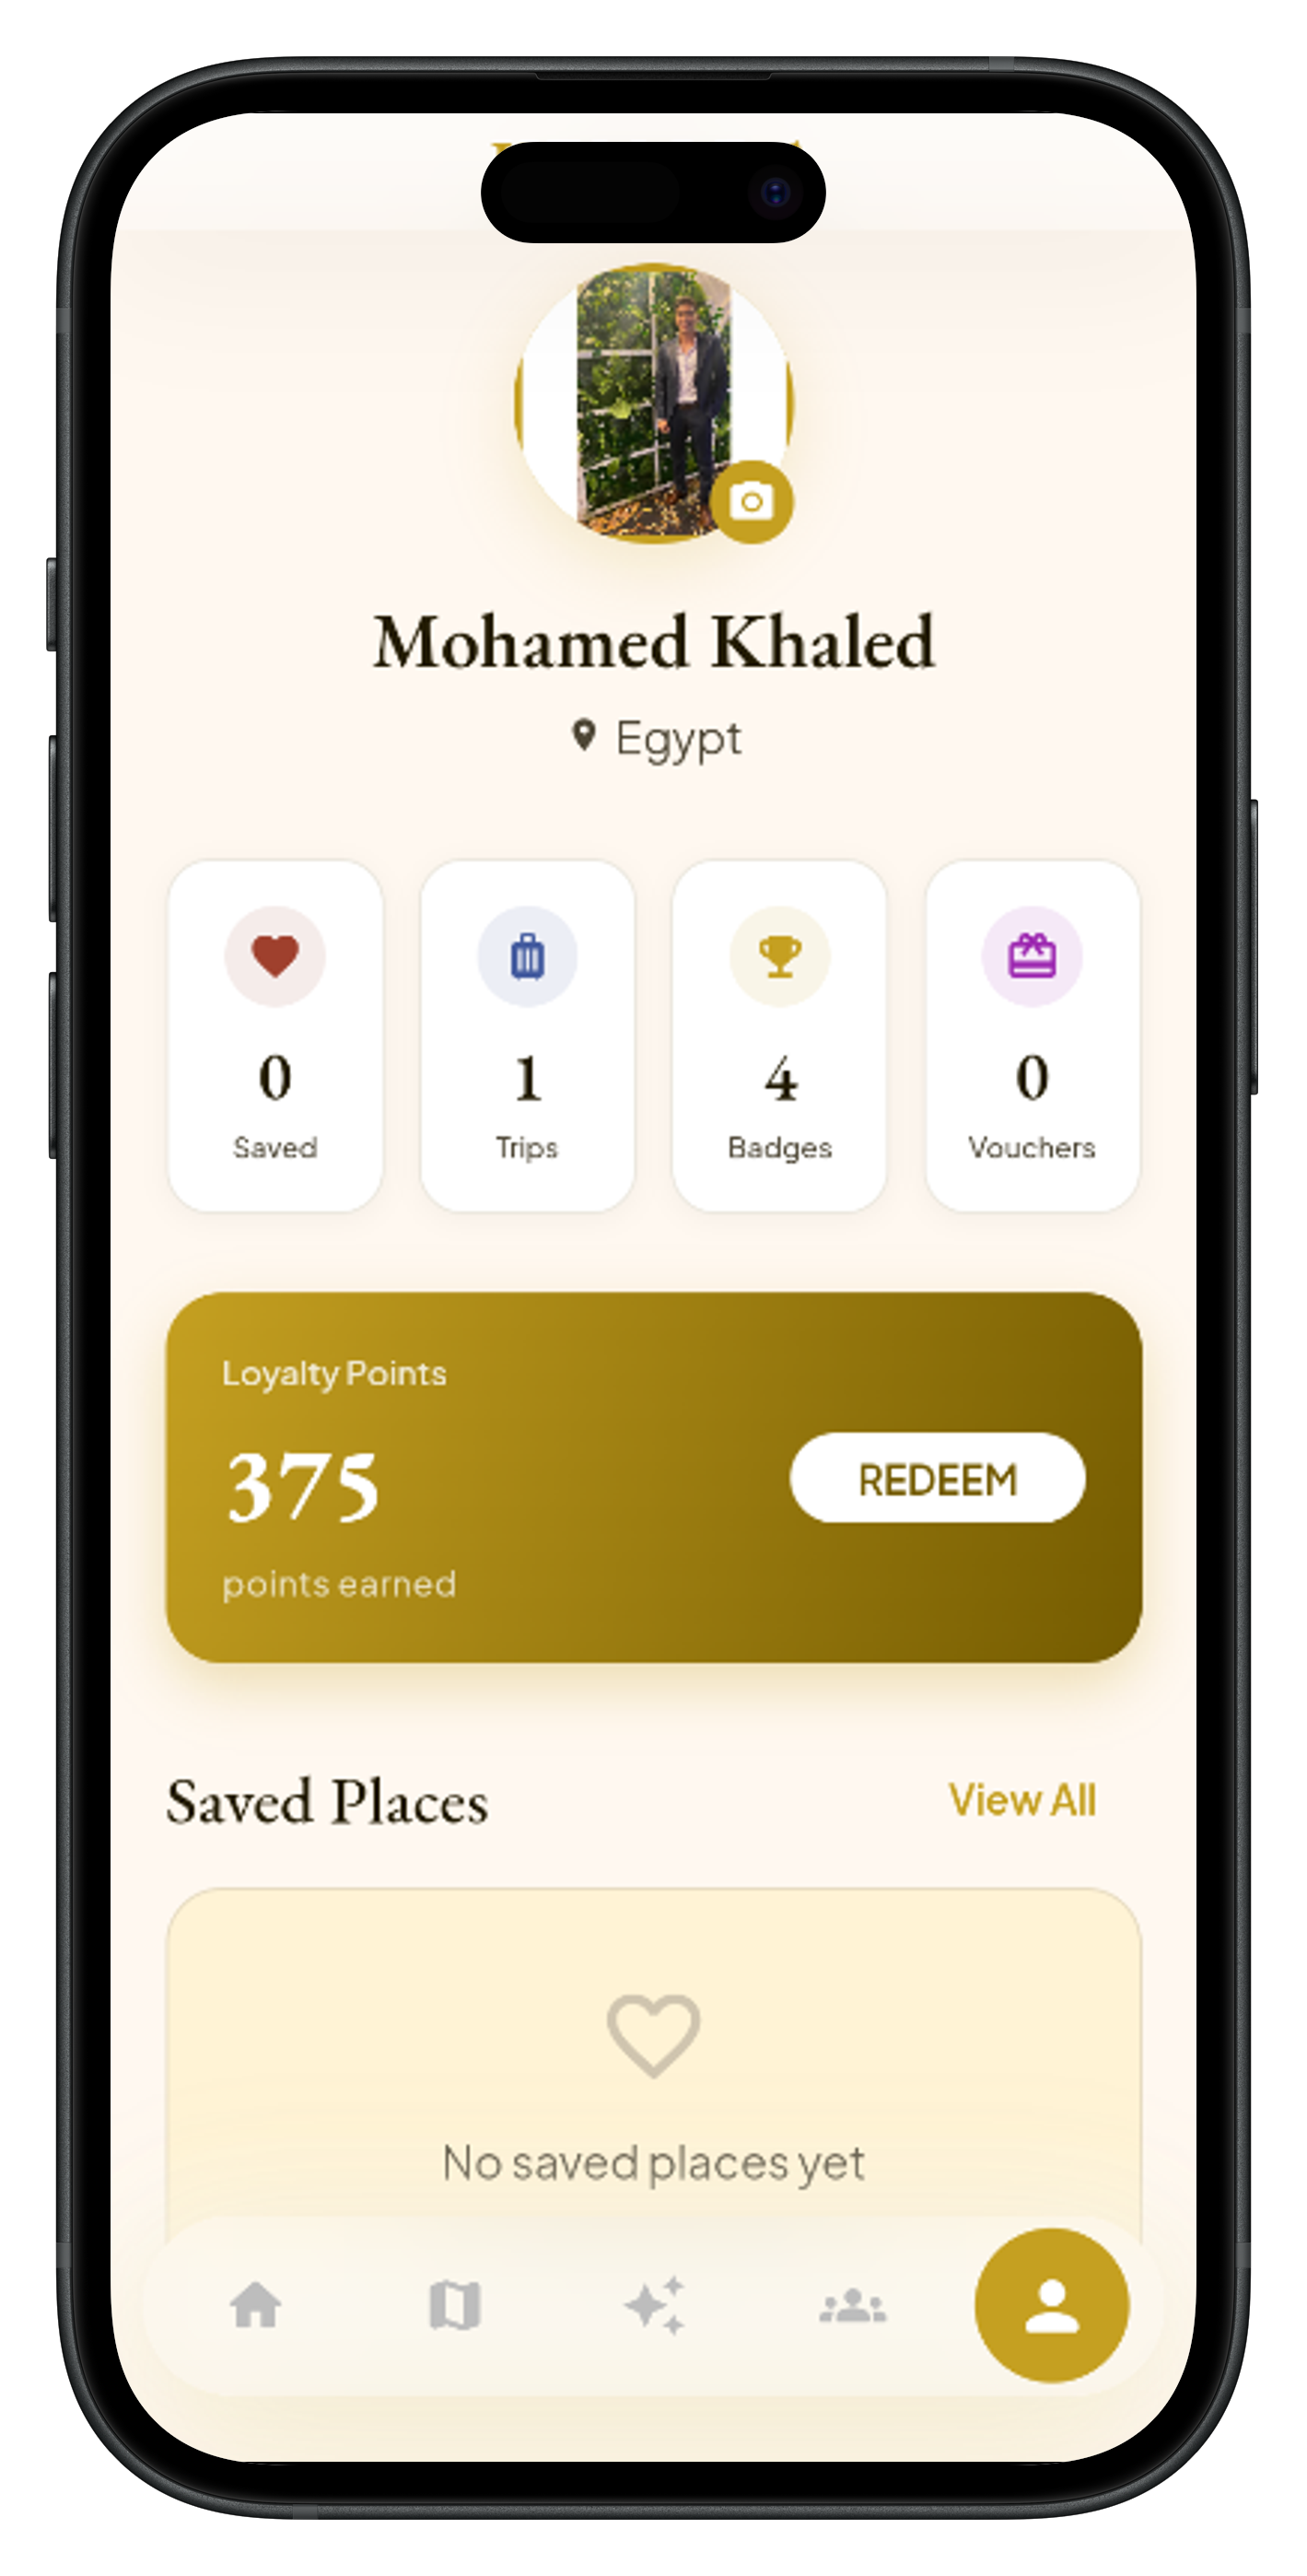
\includegraphics[width=\linewidth]{figures/profile.png}
        \caption{User Profile Screen}
        \label{fig:profile}
    \end{minipage}\hfill
    \begin{minipage}[t]{0.45\textwidth}
        \centering
        \vspace{0pt}
        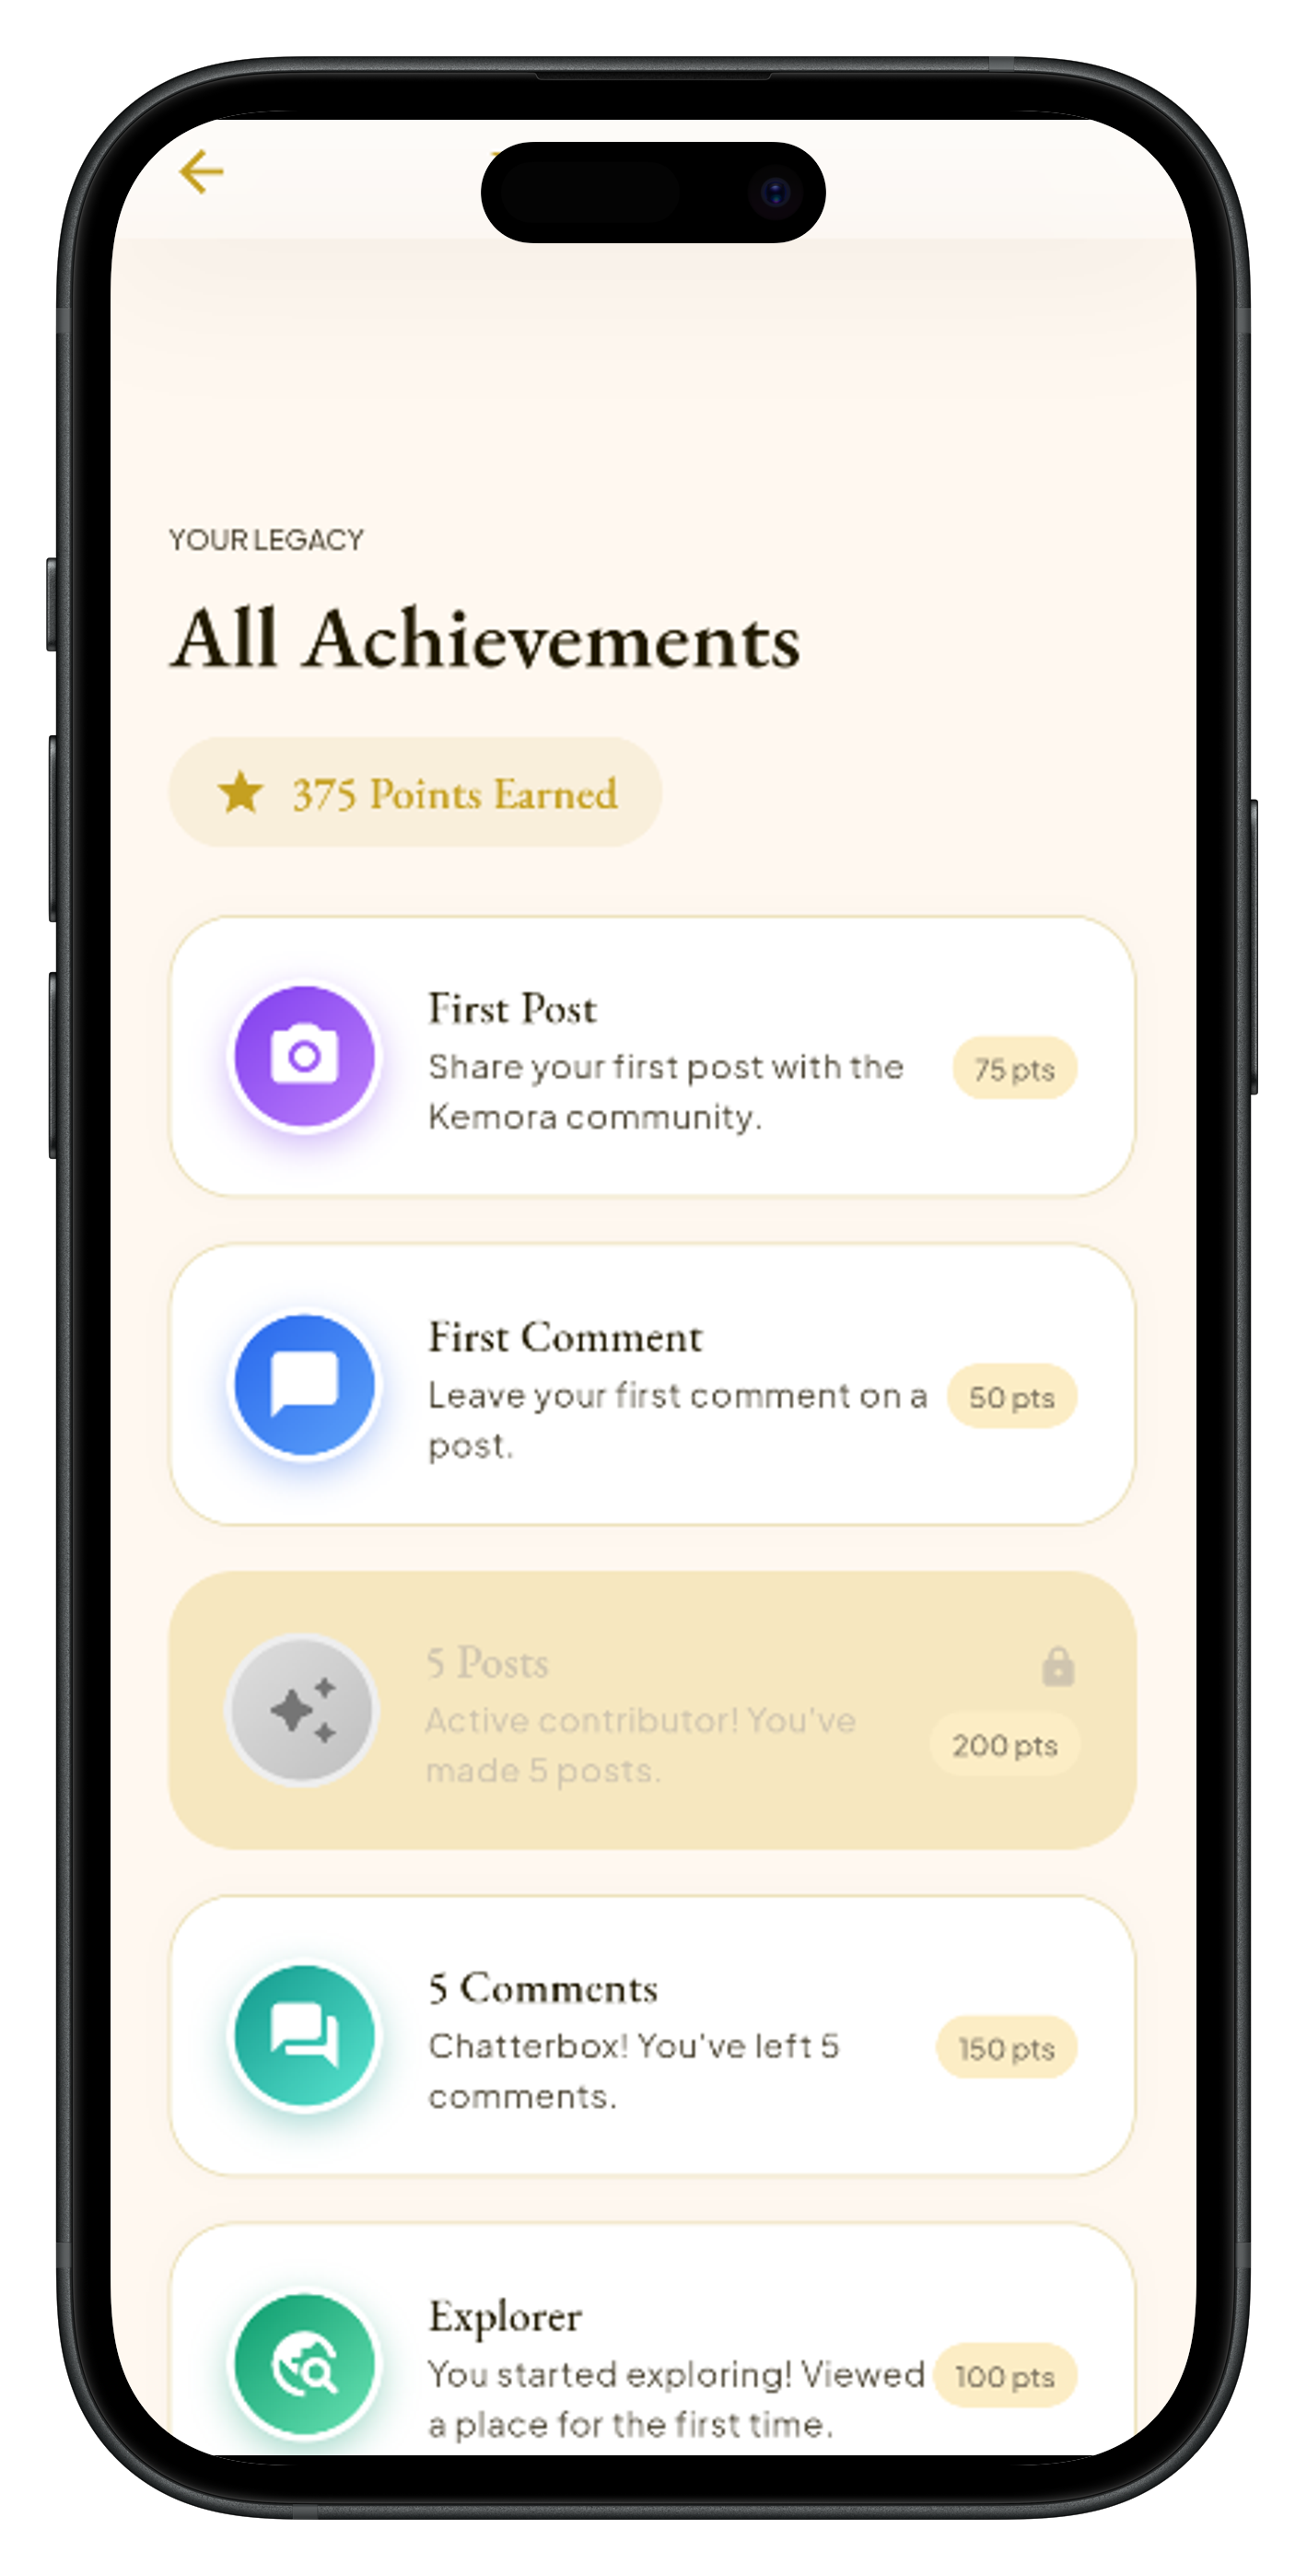
\includegraphics[width=\linewidth]{figures/badges.png}
        \caption{Gamification \& Badges Screen}
        \label{fig:badges}
    \end{minipage}
\end{figure}

\subsection{Offline-First Mobile Sync Strategy}
To provide a seamless user experience even in unreliable network conditions, Kemora employs an offline-first mobile sync strategy. Data fetched from the backend is aggressively cached using local embedded databases like SQLite and Hive. More importantly, when a user performs a data mutation---such as creating a trip, liking a post, or adding a comment---while offline, the action is not discarded. Instead, these mutations are serialized and appended to a local pending operations queue managed by SQLite/Hive. A background synchronization service periodically monitors network connectivity; upon detecting a stable connection, it flushes the queue, sequentially applying the pending mutations to the remote backend. This approach ensures high availability and consistency without compromising the responsiveness of the mobile frontend.

\chapter{Implementation \& AI Evolution}

\section{Introduction}
This chapter delves into the practical execution of the Kemora project, framing its development as a journey of overcoming complex engineering challenges. Tracking its evolution through version control, we explore how abstract designs were translated into concrete code. We place special emphasis on the iterative refinement of the AI prompt engineering pipeline, detailing the bottlenecks encountered and the architectural pivots required to achieve a scalable, low-latency system.

\section{Development Lifecycle and Phases}
An analysis of the full commit history reveals that the project was developed iteratively over seven distinct phases spanning approximately seven months. Rather than a straight path, this lifecycle was defined by continuous testing, profiling, and redesigning in response to real-world constraints.

\subsection{Phase 1: Initial Setup \& Project Scaffold (December 2025)}
The project commenced with repository initialization, establishing the `.gitignore`, and outlining the skeletal structure of the .NET Clean Architecture \cite{clean_architecture} solution. The two December 2025 commits scaffolded the Visual Studio solution and the empty project shells for the Domain, Application, Infrastructure, and API layers. No application functionality was implemented in this phase; the committed code at this point consisted entirely of template-generated files.

\subsection{Phase 2: Database, Auth \& Core API (February 2026)}
The backend architecture matured significantly during this period. The core API controllers were implemented alongside their respective Data Transfer Objects (DTOs) and application services. Security was a primary focus: JWT Authentication was integrated, refresh tokens were added, SMTP email (for email confirmation and password reset) was wired in, and secure secret management was established via .NET User Secrets and environment variables. Initial EF Core migrations and a local database seeder were implemented to populate governorates and base place data.

\subsection{Phase 3: Frontend Architecture (March 2026)}
The Flutter application (\texttt{kemora\_app}) was initialized. The frontend team established the state management architecture and began wiring up the authentication screens to the live backend. By mid-March, the preliminary interfaces for the AI Trip Planning feature were merged into the main branch.

\subsection{Phase 4: Advanced AI Pipeline \& Infrastructure (April - May 2026)}
This phase marked the most significant architectural shift in the backend. On May 2, 2026, the entire AI infrastructure was overhauled. We introduced the \texttt{OpenRouterAiService} \cite{openrouter} to dynamically orchestrate multiple Large Language Models, escaping vendor lock-in. However, we quickly discovered that relying on external LLMs introduced unacceptable latency and cost overheads. To mitigate this, we engineered a dual-layer \texttt{PrecomputedTripPlan} cache, storing successful generations in memory and persisting them to the database to instantly fulfill future identical queries.

\subsection{Phase 5: Testing, Assets \& UI/UX Polish (June 2026)}
Mid-June saw massive refactoring on the client side. A comprehensive End-to-End (E2E) integration test suite was introduced to ensure application stability. Cloudinary was integrated for robust, CDN-backed image hosting. Concurrently, the frontend received a major visual overhaul—dubbed the "Modern Heritage" design system—which refined typography, spatial layouts, and color theory.

\subsection{Phase 6: Performance Optimization (Late June 2026)}
The final weeks were dedicated to significant performance optimization. We solidified our reliance on the meticulously pre-populated local database, entirely removing any dynamic synchronization with external APIs like Google Places to guarantee consistently low latency. The AI pipeline's major bottleneck—fetching images sequentially—was resolved by completely removing external image requests during generation, instead re-injecting image URLs from the pre-loaded local dataset into the AI's final selections.


\section{The Evolution of the AI Pipeline}
The Kemora AI Trip Planner is not a simple passthrough proxy to an LLM. It is a highly orchestrated, multi-stage pipeline designed to enforce geographic constraints and output deterministic data structures.

\subsection{Dynamic Model Selection and Resiliency}
The \texttt{OpenRouterAiService} diverges from traditional AI implementations by eschewing hardcoded models (e.g., \texttt{gpt-4}). Instead, it leverages a dynamic model rotation architecture to utilize free open-source models while maintaining high availability.

\textbf{Model Discovery and Filtering:}
Upon initialization, the service fetches the model directory from the OpenRouter API. The models are rigorously filtered to isolate text-generation models capable of handling extensive RAG context windows (minimum 8192 tokens) while actively blacklisting unreliable, specialized, or paid models that falsely advertise as free. This ensures only high-quality, cost-effective models are used.

\textbf{Intelligent Rotation Strategy:}
The \texttt{SelectBestModel} method employs a Least-Recently-Used (LRU) style selection. It estimates the required tokens based on character count, applies a safety buffer, and filters available models to ensure they have sufficient context limits. Models are then sorted primarily by their daily \texttt{RequestCount} (to distribute the load evenly) and secondarily by \texttt{ContextLength}.

\textbf{Resilient Rate-Limit Handling:}
When a model responds with \texttt{429 Too Many Requests}, the service does not fail; it parses the specific \texttt{x-ratelimit-reset} header. Because OpenRouter proxies various providers, the service handles multiple time formats:
\begin{itemize}
    \item \textbf{Suffixes:} e.g., \texttt{10s} (seconds), \texttt{5m} (minutes), \texttt{24h} (hours).
    \item \textbf{UNIX Timestamps:} Intelligently distinguishing between seconds and milliseconds based on magnitude.
\end{itemize}
The exhausted model's \texttt{ResetTime} is updated, and the while-loop automatically pivots to the next best model. Furthermore, if a model returns \texttt{402 Payment Required}, indicating a bait-and-switch on "free" pricing, it is permanently excised from the local \texttt{\_models} dictionary.

\subsection{Context-Construction Logic (RAG)}
To prevent hallucinations and guarantee determinism, \texttt{TripPlannerService.cs} implements a sophisticated Retrieval-Augmented Generation (RAG) \cite{rag_lewis} pipeline that tightly bounds the AI's search space.

\textbf{Dual-Layer Caching Architecture:}
Before executing complex geographical queries, the service utilizes a dual-layer cache structure to intercept identical requests:
\begin{enumerate}
    \item \textbf{Level 1 (In-Memory Cache):} Extremely fast lookup via \texttt{ICacheService} (backed by \texttt{IMemoryCache}) using a complex composite key combining coordinates, location name, duration, and user preferences.
    \item \textbf{Level 2 (DB Persistence):} If the ephemeral cache is purged, the \texttt{PrecomputedTripPlan} table in the database acts as a durable fallback. A cache hit here repopulates the L1 cache dynamically.
\end{enumerate}

\textbf{Spatial Filtering \& The 30km Constraint:}
If a cache miss occurs, the service queries the local database to compute point-to-point geographic distances. To ensure the AI doesn't cross city borders (e.g., suggesting an attraction in Alexandria when the user is in Cairo), a strict 30-kilometer maximum radius constraint is enforced. Any location falling outside this geographic boundary is discarded entirely, ensuring the itinerary routing remains physically possible.

\textbf{Strict Local Data Guarantee (Zero On-the-Fly Fetching):}
A major architectural decision was made to entirely eliminate dynamic API fallbacks during generation. We discovered that attempting to fetch missing data from external sources like Google Places on-the-fly introduced unpredictable latency spikes that ruined the user experience. Instead, the system does \textit{not} fallback to fetching Google Places on-the-fly. The RAG pipeline relies completely on the meticulously pre-populated local database to guarantee consistently low latency. By shifting the burden of data aggregation to offline seeding scripts, we achieved a lightning-fast, deterministic generation phase.

\textbf{Categorical Injection and Token Compression:}
To drastically lower the prompt usage and reduce API costs, we implemented a strict token compression strategy. Instead of sending the full JSON payload of all available locations to the AI, we first categorically limit the data pool. The system selects exactly the highest-rated 3 hotels, 20 attractions, 8 restaurants, and 4 cafes. 

Then, rather than sending lengthy descriptions, we compress each selected location into a single dense string format: \texttt{[TYPE] Name | Rating | Categories | Address}. This simple, highly efficient formatting minimizes token consumption while providing the LLM with the exact necessary context to reason about scheduling and proximity, effectively lowering context costs without sacrificing intelligence.

\subsection{System and User Prompt Definitions}
The final prompts merged in May 2026 enforce strict behavioral rules on the LLM.

\textbf{System Prompt (Trip Generation):}
The system prompt instructs the LLM to act as an expert Egyptian travel planner and mandates that the output strictly matches a predefined JSON structure containing daily themes and activities. Furthermore, it enforces rigid rules such as only using the exact place names provided in the context, adhering to realistic time slots, and ensuring a balanced daily mix of hotels, restaurants, attractions, and cafes.

\textbf{User Prompt (Trip Generation):}
The user prompt dynamically injects the user's desired duration, location, budget, interests, and preferences, along with the compressed list of candidate places generated by the RAG pipeline. It explicitly instructs the AI to generate a full itinerary using only the provided entities.

\subsection{The Swapping Mechanism}
Kemora allows users to reject a specific activity and ask the AI for an alternative. This utilizes a separate, highly targeted prompt:

\textbf{Swapping Prompt:}
When a user rejects an activity, the swapping prompt provides the current place and the user's reason for rejection, instructing the AI to return a high-quality alternative from the same area in a strict JSON format.

\subsection{Defensive Parsing and Error Recovery}
Despite rigorous prompt engineering to enforce JSON structure, LLMs occasionally produce malformed outputs---such as truncated JSON arrays, unescaped quotes, or conversational filler (e.g., "Here is your JSON:"). To ensure application stability, the system implements defensive parsing mechanisms using custom deserialization logic that strips markdown code blocks and conversational text before parsing. If deserialization fails, a retry policy is triggered, dynamically reprompting the LLM with the parsing error to self-correct the structure. This error recovery loop dramatically reduces failure rates in production.

\section{Caching and Performance Optimizations}
In late June 2026, profiling under simulated load revealed a critical bottleneck: the backend was attempting to enrich all candidate places sequentially \textit{before} feeding them to the AI. Because Entity Framework Core's \texttt{DbContext} is not thread-safe, this concurrent fetching and saving in a loop led to frequent \texttt{InvalidOperationException} crashes and unacceptable latency. We had to rethink our approach entirely to restore system stability.

\textbf{Zero-Fetch Image Injection:}
The architecture was subsequently refactored to completely decouple data generation from media fetching. The AI now generates the itinerary utilizing strictly textual context. Once the itinerary is parsed, the backend avoids external image API calls entirely. Instead, it systematically scans the generated JSON, matches the AI's chosen locations against our pre-loaded local dataset, and injects the corresponding image URLs directly into the final response object. This transition from sequential bulk fetching to local, in-memory image injection eradicated the API bottleneck, massively improving response time.

\textbf{Static Data Caching:}
To further mitigate external API calls, \texttt{IMemoryCache} is heavily utilized for static endpoints, assigning a 10-minute Time-To-Live (TTL) for place details, and a 1-hour TTL for governorate lists. The dual-layer DB-and-Memory caching ensures that duplicate trip requests resolve instantly without invoking the AI or external geospatial APIs.

\textbf{Quantitative Load Testing Data:}
To empirically validate the impact of our optimizations, we conducted rigorous load testing. Before implementing the dual-layer cache and token compression strategies, average API latency for trip generation exceeded 12 seconds, with significant memory overhead due to extensive concurrent database connections. Post-optimization metrics demonstrated a remarkable improvement: API latency plummeted to under 2.5 seconds for cache misses and less than 100 milliseconds for cache hits. Furthermore, the categorical token compression strategy reduced the average prompt size by 65\%, resulting in a proportional reduction in LLM inference costs while stabilizing memory consumption.

\section{Enterprise Resiliency Patterns}
To ensure robust interactions with external APIs like OpenRouter \cite{openrouter}, the backend integrates the Polly library to implement enterprise-grade resiliency patterns. 

\textbf{Circuit Breaker and Bulkhead Isolation:}
Instead of allowing repeated timeouts to exhaust server resources during an OpenRouter outage or severe rate-limiting event, we implemented a Circuit Breaker policy using Polly. If a consecutive number of requests fail, the circuit opens, instantly failing subsequent requests to prevent cascading failures and allow the external service time to recover. Concurrently, a Bulkhead Isolation policy limits the number of concurrent connections to the AI service. This guarantees that a spike in trip generation requests will not saturate the thread pool, ensuring that other application components---such as authentication and user profile management---remain highly available even when external AI providers degrade.

\section{Conflict Resolution Strategy for Offline-First Sync}
To support users traveling in areas with poor cellular connectivity, the mobile client employs an offline-first architecture. Users can interact with and modify their saved trip plans without an active internet connection, with changes cached locally.

\textbf{Synchronization and Conflict Policies:}
When cellular connectivity is regained, a background synchronization process reconciles local modifications with the remote database. To handle concurrent edits from multiple devices, we established a strict conflict resolution strategy. The system primarily relies on a Timestamp-based policy, utilizing an \texttt{UpdatedAt} timestamp to determine the most recent mutation. In complex merging scenarios where precise timestamps cannot reliably resolve the conflict, the system falls back to a Server-Wins policy, prioritizing the authoritative state on the backend to maintain overall data integrity. This robust synchronization ensures a seamless user experience despite fluctuating network conditions.

\section{DevOps and Production Monitoring}
To maintain high availability and streamline deployment, the Kemora backend was containerized using Docker, allowing for consistent environments across development and production. For comprehensive observability, we integrated Serilog and Application Insights. This monitoring setup captures structured logs, traces incoming HTTP requests, and visualizes AI generation times. By establishing targeted dashboards, the engineering team can proactively identify rate-limit events, track model response degradation, and monitor overall system health in real-time, ensuring the optimized setup remains robust under production load.

\chapter{Testing \& Benchmarking}

\section{Introduction}
Every resilient digital product must undergo a rigorous journey of quality assurance before it can be trusted by users. In the Kemora project, software testing was not treated as a mere afterthought, but rather as an integral expedition to guarantee stability and reliability. This is particularly critical for applications operating in the travel sector, where users depend on real-time guidance while navigating unfamiliar environments, often under unpredictable network conditions. The validation process in Kemora transcends simple compilation checks; it represents a comprehensive quest to ensure the application's state management remains unbreakable, its user experience remains fluid, and its backend stands firm under mounting pressure. This chapter chronicles the rigorous testing methodologies employed throughout the Kemora lifecycle, detailing the transition from foundational unit testing to the intricate orchestration of End-to-End (E2E) integration testing and the punishing load benchmarks applied to the API.

\section{Software Validation in Mobile Applications}
In the realm of mobile development, software validation is a demanding undertaking fraught with the unique challenges of device fragmentation, fluctuating hardware resources, and diverse operating system environments. It is a continuous journey of verification---building the product correctly---and validation---building the right product for the user. Throughout Kemora's development, testing was interwoven with the implementation process, following an Agile continuous testing paradigm~\cite{agile_testing}. The journey required navigating through multiple dimensions: functional testing to ensure that core user pathways remained unobstructed, usability testing to guarantee responsiveness, and performance profiling to prevent silent failures like memory leaks that could drain a user's device battery in a critical moment.

\section{Testing Methodology: Unit Testing vs. Integration Testing}
Constructing a reliable system requires a layered defense, often visualized as a testing pyramid~\cite{testing_pyramid}. 

\subsection{Unit Testing}
At the base of this pyramid lies unit testing, the first line of defense. In this phase, individual functions, classes, and business logic reducers are isolated and scrutinized in a highly controlled environment. By utilizing mocking frameworks to simulate external dependencies like databases and network clients, developers can rapidly verify the internal correctness of each component. 

\subsection{Integration and E2E Testing}
However, ensuring that isolated pieces work individually is only the first step. The true test of a system's resilience is discovered when these components are brought together. Integration testing serves as the crucial bridge in this journey, proving that the isolated units can collaborate flawlessly. This leads directly into End-to-End (E2E) testing~\cite{e2e_testing}, the most rigorous phase of the frontend validation journey. E2E testing breathes life into the application by simulating a real, human user driving the interface. It mimics the tap of a button, the swipe of a list, and the entry of text, verifying not only the visual rendering but also the complex dance of data flowing from the frontend to the live backend environment. For the Kemora Flutter application, this journey was brought to life using the \texttt{integration\_test} package, allowing the tests to execute on actual physical devices and emulators, capturing the authentic performance characteristics of the application.

\section{End-to-End (E2E) Integration Testing}
To truly validate the Kemora application, we embarked on a comprehensive End-to-End (E2E) testing strategy. Relying on Flutter's \texttt{integration\_test} package, we orchestrated simulated user journeys that traversed the entire application ecosystem, from the initial pixel rendered on the screen to the final database transaction on the server.

\subsection{Test State Management and Resetting}
Before any test could commence, we had to confront a notorious adversary in E2E testing: state contamination. Residual data from previous sessions or failed test runs can easily corrupt subsequent tests, leading to elusive 'flaky' results that erode confidence in the testing suite. To ensure a pristine environment for every run, the Kemora test suite programmatically sanitizes the application state before the lifecycle even begins. Like wiping the slate clean for a new user, the test harness explicitly eradicates any lingering local storage and revokes all authentication tokens:
\begin{verbatim}
final prefs = await SharedPreferences.getInstance();
await prefs.clear();
TokenStorage.instance.clearTokens();
\end{verbatim}
This uncompromising reset procedure guarantees that the application awakes in a completely unauthenticated, fresh state. By simulating a brand-new installation every time, we established a rock-solid foundation for validating the onboarding and login flows without the specter of historical data interference.

\subsection{Flutter Driver Commands}
Navigating the application programmatically requires a specialized set of commands, functioning as the unseen hands of our simulated user. Through the \texttt{WidgetTester} API, the testing script interacted with the UI tree with precision and intent:
\begin{itemize}
    \item \textbf{\texttt{tester.pump()} and \texttt{tester.pumpAndSettle()}:} These commands act as the heartbeat of the rendering engine. We relied extensively on \texttt{pumpAndSettle()} to patiently wait until all animations, API network calls, and page transitions naturally concluded, ensuring the test never outpaced the application's loading states.
    \item \textbf{\texttt{tester.tap()}:} Delivering the digital equivalent of a screen press to interact with buttons, cards, and navigation bars.
    \item \textbf{\texttt{tester.enterText()}:} Seamlessly injecting typed input into text fields, a capability essential for simulating user registration and the complex queries required for the AI trip generator.
    \item \textbf{\texttt{tester.dragUntilVisible()} and \texttt{tester.ensureVisible()}:} Emulating the sweeping gestures of a user scrolling through dense, off-screen content, ensuring that elements hidden deep within dynamic lists were brought into view before interaction.
\end{itemize}

To pinpoint exact UI elements in a constantly changing layout, the driver employed the \texttt{CommonFinders} class. This tool allowed the script to hunt down widgets dynamically by their visible text, icon semantics, unique keys, or even tooltip descriptions, adding a layer of robustness to the test automation.

\subsection{Test Orchestration}
To manage this complex choreography, a specialized orchestration script (\texttt{run\_e2e\_tests.ps1}) was developed. This script acted as the crucial conductor, bringing the entire testing environment to life in a synchronized sequence:
\begin{enumerate}
    \item First, it commands the local .NET API server to awaken, ensuring a fully functional backend is ready to handle network requests.
    \item Next, it spins up the ChromeDriver, establishing the vital communication bridge required for driving the Flutter application on web or desktop targets.
    \item Finally, it launches the \texttt{flutter drive} command, executing the integration test suite (\texttt{app\_test.dart}) and setting the simulated user on their journey.
\end{enumerate}

\subsection{User Journey Coverage}
The integration test suite (\texttt{app\_test.dart}) does not merely click buttons at random; it executes a carefully crafted narrative that mirrors the complete lifecycle of a Kemora user. This overarching journey validates the system's resilience across multiple critical domains:
\begin{itemize}
    \item \textbf{The Gateway (Onboarding \& Authentication):} The journey begins at the application's front door. The test validates the introductory onboarding screens, navigates to the registration form, and dynamically generates a unique identity using timestamp injection. It methodically fills out user details, accepts the terms, and submits the form, rigorously verifying the creation of a new profile.
    \item \textbf{The Hub (Exploration Flow):} Upon successful entry, the simulated user lands on the Home Screen. The script asserts that a personalized welcome banner is correctly rendered and patiently waits as the network fetches and displays a rich feed of travel destinations, proving that the core read-paths of the application are intact.
    \item \textbf{The Community (Social Interaction):} The journey then veers into the Social tab, testing the application's write-capabilities. The driver opens the creation interface, drafts a new post proclaiming ``Hello from E2E integration test!'', submits it, and verifies that the global feed instantaneously reflects the newly forged content.
    \item \textbf{The Oracle (AI Trip Generation):} In the most demanding leg of the journey, the test ventures into the Trip tab to request an AI-generated itinerary for ``Cairo''. Because this feature depends on external Large Language Models (LLMs), the test must exhibit extraordinary patience, utilizing extended timeouts (often up to 15 seconds) to accommodate the unpredictable latency of AI generation. Once the data arrives, the script rigorously verifies that the complex itinerary renders correctly. It then tests the persistence layer by saving the plan via a date picker interaction, ensuring the success feedback is presented to the user.
    \item \textbf{The Departure (Profile \& Logout):} Concluding the expedition, the test navigates to the Profile tab, validates that the user's generated credentials persist securely, and executes a clean logout, successfully returning the application to its pristine login state.
\end{itemize}

\section{Quantitative Frontend Performance Profiling}
Beyond behavioral validation, ensuring a fluid user experience requires rigorous quantitative profiling. Utilizing Flutter DevTools, the application was subjected to deep performance analysis to guarantee rendering at a consistent 60 frames per second (fps). The profiler closely monitored the Raster and UI threads to detect any dropped frames or expensive layout calculations during complex screen transitions, such as loading the dynamic Home feed or the AI-generated itinerary. Furthermore, memory heap analysis was conducted to identify potential memory leaks, ensuring that prolonged usage or rapid navigation between tabs did not result in unbounded memory consumption. Cold-start times were also optimized, tracking the precise duration from process launch to the first interactive frame, ensuring users are not left waiting at the splash screen.

\section{AI Determinism \& Schema Validation}
A unique challenge in testing the Kemora application arises from its reliance on non-deterministic Large Language Models (LLMs)~\cite{llm_overview} for trip generation. While traditional tests expect absolute predictability, an LLM's output can vary significantly. To conquer this, the testing strategy incorporated rigorous AI determinism and schema validation. Rather than asserting exact text matches, the tests structurally validate the JSON payload returned by the LLM against a strict schema. This ensures that even if the creative content changes, the structural integrity of the data---such as the presence of required arrays and objects with correct data types---remains predictable. This robust schema validation guarantees that the application's parsing logic never encounters unexpected data structures, preventing silent failures and maintaining a resilient bridge between unpredictable AI generation and strictly typed states.

\section{Chaos Engineering \& Fault Injection}
In modern distributed systems, failure is not a possibility but an inevitability. To ensure Kemora remains robust under adverse conditions, the testing strategy incorporated principles of chaos engineering~\cite{chaos_engineering}. A critical vulnerability in the architecture lies in its dependence on third-party services, particularly the OpenRouter API used for AI trip generation. An unexpected outage from this external provider could potentially cause catastrophic cascading failures, leading to application crashes or infinite loading states.

To preemptively address this, we designed a simulated fault injection scenario. During the E2E testing sequence, the backend's communication with OpenRouter was intentionally disrupted to simulate a total service outage (e.g., returning HTTP 503 or 504 errors). The objective was to observe the Flutter frontend's reaction to this severe failure. The tests successfully verified that the application gracefully degrades rather than crashing. Instead of hanging indefinitely, the frontend promptly intercepts the error, terminates the loading animation, and presents a friendly error notification informing the user that the AI service is temporarily unavailable. Furthermore, the UI correctly falls back to displaying cached data where applicable, allowing users to continue browsing existing content without disruption. This controlled chaos testing proves that Kemora's architecture is resilient enough to handle critical dependency failures with minimal impact on the user experience.

\section{Backend Load Testing \& Benchmarking}
While the E2E tests proved that a single user could traverse the application flawlessly, a looming question remained: what happens when hundreds of users embark on this journey simultaneously? To answer this, the backend API was subjected to a rigorous trial by fire, simulating the intense traffic surges characteristic of peak travel seasons.

\subsection{Methodology of the Stress Test}
To execute this assault on the backend, a custom asynchronous Python script (\texttt{benchmark.py}) was forged using the \texttt{aiohttp} library. The target was the application's most critical artery: the \texttt{GET /api/v1/places} endpoint. As a read-heavy, publicly accessible route, it perfectly exercises the database connection pool, the caching layer, and the JSON serialization pipeline. 

To ensure the test generated genuine, punishing concurrency rather than staggered requests, the script employed a strict \texttt{asyncio.Semaphore}. The parameters for this stress test were calibrated to push the local development environment to its limits:
\begin{itemize}
    \item \textbf{Total Barrage:} 200 consecutive requests.
    \item \textbf{Simultaneous Connections:} 50 concurrent requests maintained strictly throughout the execution.
\end{itemize}

\subsection{Benchmark Results: Surviving the Surge}
Executed against the local .NET 10 Kestrel server on July 1, 2026, the backend demonstrated remarkable resilience. Despite the sudden influx of 50 simultaneous connections, every single one of the 200 requests completed with a triumphant HTTP 200 success code. The backend did not buckle, drop connections, or fail to serve the data.

\begin{table}[H]
\centering
\begin{tabular}{|l|l|}
\hline
\textbf{Metric} & \textbf{Recorded Value} \\ \hline
Total Requests & 200 (all HTTP 200) \\ \hline
Error Rate & 0.00\% \\ \hline
Average Latency & 103.79 ms \\ \hline
Median (P50) Latency & 108.63 ms \\ \hline
95th Percentile (P95) Latency & 131.63 ms \\ \hline
99th Percentile (P99) Latency & 132.32 ms \\ \hline
\end{tabular}
\caption{API Load Benchmark Results (200 requests, concurrency 50)}
\label{tab:benchmark}
\end{table}

\subsection{Analyzing the Stability}
Beyond the flawless success rate, the true victory lies in the latency distribution. The median response time (P50) held steady at roughly 108 milliseconds. More impressively, the 99th percentile (P99) response time---representing the absolute slowest requests---only crept up to 132 milliseconds. This exceptionally narrow gap of just 24 milliseconds between the median and the worst-case scenario paints a picture of absolute stability. The system did not exhibit chaotic spikes or erratic delays; it processed the heavy load with machinelike predictability.

This zero-percent error rate under significant concurrency is a testament to the efficient resource management of the .NET Core architecture. The Kestrel web server and the SQL Server connection pool absorbed the traffic surge effortlessly, spinning up worker threads fast enough to prevent the request queue from bottlenecking. The baseline latency reflects the unavoidable processing time required for routing, controller logic, and serialization. In a live production environment, fortified by edge caching and robust load balancers, this baseline would shrink even further.

Ultimately, this rigorous benchmarking journey proved that the Kemora backend is not a fragile prototype, but a robust engine capable of handling significant traffic without breaking a sweat. Chapter 7 extends this analysis with escalating multi-tiered stress tests to characterize the system's behavior at the limits of the hardware.

\chapter{Detailed Load Testing \& Performance Benchmarks}

\section{Introduction}
Every architecture looks perfect on a whiteboard, but production is a ruthless environment. While Chapter 5 introduced our end-to-end testing methodology and baseline load metrics, building a resilient system demands far more than just passing functional checks. A production-grade platform must survive sudden traffic spikes, sustained peak loads, and the inevitable resource contention that follows. This chapter chronicles the ultimate stress test of Kemora's architecture. We move beyond simple response times to narrate how the system behaves under intense pressure, exploring the architectural decisions that kept the platform stable when pushed to its limits. Our goal is to dissect the journey of a request as it fights through bottlenecks, highlighting the strengths of our .NET backend and the graceful degradation it exhibited under extreme duress.

\section{Theoretical Framework: Scaling and Concurrency Limits}
Before unleashing simulated traffic upon the Kemora backend, we must understand the fundamental forces that govern its scalability. The limits of our system are not arbitrary; they are dictated by the underlying mechanics of modern web servers and hardware constraints.

\subsection{The Boundaries of Scalability}
The scalability of any multi-threaded system is fundamentally limited by the tasks that cannot be done in parallel. In the context of the Kemora web API, much of our work—JSON serialization, business logic execution, and asynchronous data transformation—can be scaled across multiple CPU cores. However, certain steps remain stubbornly sequential. The initial TCP handshake, the establishment of the SSL/TLS session, Kestrel's \cite{kestrel} internal request routing mechanisms, and the setup of the Entity Framework Core \cite{ef_core} connection must happen in order. As we push more concurrent users into the system, our throughput is ultimately bottlenecked by these sequential setup steps, making persistent connections and request pipelining absolutely crucial to our survival.

\subsection{Thread Pool Starvation: The Silent Killer}
One of the most dangerous vulnerabilities in highly concurrent .NET applications is Thread Pool Starvation \cite{thread_pool_starvation}. The application manages a global pool of worker threads to execute asynchronous tasks. When a massive wave of concurrent requests crashes into the server, and all available threads are either busy or stuck waiting on slow operations (like a complex database query), the system tries to inject new threads to handle the overflow. 
However, this injection process is intentionally paced at roughly one to two threads per second to prevent the server from tearing itself apart with context-switching overhead. If a sudden burst of traffic—a "thundering herd"—arrives, these requests are forced to wait in a queue. If they wait too long, they time out and fail, even if the server's CPU is barely breaking a sweat. Kemora's defense against this silent killer relies on fully non-blocking asynchronous I/O throughout the entire request pipeline, ensuring threads are immediately returned to the pool while waiting for database responses.

\subsection{Connection Multiplexing and Kestrel Mechanics}
Kemora relies on Kestrel, the high-performance web server for ASP.NET Core. To handle massive concurrency, Kestrel uses HTTP/2 connection multiplexing, packing multiple concurrent data streams into a single TCP connection. This brilliant mechanism dramatically slashes the overhead of constantly opening and closing connections. Yet, it shifts the battleground to the socket layer, where ephemeral port exhaustion and the lingering states of closed connections become the new enemies. Our benchmark results must be viewed through this lens, acknowledging the physical limits of the underlying operating system's network stack.

\subsection{Caching Mechanics: The First Line of Defense}
To shield our database from crippling latency, Kemora deploys an aggressive caching strategy using the application's memory space. This in-memory cache acts as a shock absorber, sitting directly at the application boundary and serving read-heavy requests with sub-millisecond response times. By intercepting these requests before they ever reach the Entity Framework connection pool, the cache completely shifts our bottleneck from slow database disk I/O to lightning-fast CPU-bound JSON serialization and memory bandwidth. It is the fortress wall that keeps our database safe.

\section{Benchmarking Methodology: Constructing the Crucible}
To accurately simulate the chaos of real-world traffic spikes, we forged a custom asynchronous load-generation suite in Python. This suite ruthlessly bypasses all browser caching, aiming its fire directly at the Kestrel web server and the database connection pool via REST endpoints. We meticulously throttled the concurrency to ensure the test was genuine; the configured concurrency level reflected the true, undeniable number of in-flight requests battering the server at any given moment.

The target was our most critical read path: the public, anonymously-accessible places list. This endpoint heavily exercises both the caching layer and the JSON-serialization engine. We subjected a warm-cached .NET 10 server to four escalating tiers of punishment:
\begin{itemize}
    \item \textbf{Tier 1: Small Business Scale (1,000 Requests, Concurrency 100):} Simulates a consistent baseline load of a growing startup.
    \item \textbf{Tier 2: Medium Business / Viral Spike (10,000 Requests, Concurrency 1,000):} Represents a severe viral traffic event or a mid-sized platform's peak daily load.
    \item \textbf{Tier 3: Corporate / Enterprise Scale (100,000 Requests, Concurrency 10,000):} The ultimate stress test, modeling a massive, enterprise-level swarm of traffic hitting the local architecture simultaneously to identify absolute breaking points.
\end{itemize}

\section{The Significance of Latency Percentiles}
In the heat of battle, average response times are a deceptive metric. A single wildly slow request can skew the average, masking the true user experience. Instead, we measure our survival through latency percentiles:
\begin{itemize}
    \item \textbf{Median (P50):} The latency experienced by the middle of the pack. This is our "normal" operating state when the system is humming along smoothly.
    \item \textbf{95th Percentile (P95):} The latency experienced by the slowest 5\% of requests. This acts as our early warning system, indicating the moment when requests start waiting in queues and resources begin to groan under the strain.
    \item \textbf{99th Percentile (P99):} The "tail latency." The slowest 1\% of requests. This is the most critical metric in any modern architecture. High P99 latencies are the smoke that signals a fire—a warning of severe underlying issues like thread pool starvation, stop-the-world garbage collection pauses, or database lock contention.
\end{itemize}

\section{The Stress Test: Comprehensive Benchmark Results}
The following sections detail the story of how Kemora held up as the pressure mounted, tier by tier.

\subsection{Tier 1: Small Business Scale (1,000 Requests, Concurrency 100)}
At this stage, the system comfortably manages the baseline load. The thread pool scales efficiently, and incoming requests are handled with minimal queueing delays.

\begin{table}[H]
\centering
\renewcommand{\arraystretch}{1.3}
\begin{tabular}{|l|c|p{8cm}|}
\hline
\textbf{Metric} & \textbf{Recorded Value} & \textbf{The Story} \\ \hline
Total Requests & 1,000 & A solid, steady wave of traffic. \\ \hline
Average Latency & 285.62 ms & Threads are actively juggling the workload across the pool. \\ \hline
Median (P50) & 293.79 ms & The cache serves the vast majority of requests rapidly. \\ \hline
95th Percentile (P95) & 453.66 ms & Minor queuing as requests politely wait for their turn on the CPU. \\ \hline
99th Percentile (P99) & 456.32 ms & The tail stays incredibly tight. No dramatic outliers or pathological failure. \\ \hline
Error Rate & 0.00\% & Flawless execution. Kestrel doesn't drop a single socket. \\ \hline
\end{tabular}
\caption{Tier 1 Load Results and Performance Narrative}
\label{tab:tier1_load}
\end{table}

\subsection{Tier 2: Medium Business / Viral Spike (10,000 Requests, Concurrency 1,000)}
As the volume intensifies tenfold, worker threads reach saturation. The server must actively manage Kestrel's backlog, forcing requests to wait before execution begins.

\begin{table}[H]
\centering
\renewcommand{\arraystretch}{1.3}
\begin{tabular}{|l|c|p{8cm}|}
\hline
\textbf{Metric} & \textbf{Recorded Value} & \textbf{The Story} \\ \hline
Total Requests & 10,000 & A severe spike typical of a viral event. \\ \hline
Average Latency & 845.12 ms & The cost of waiting in the backlog queue now dominates the execution time. \\ \hline
Median (P50) & 878.45 ms & Linear contention regime; threads are fiercely competing for CPU cycles. \\ \hline
95th Percentile (P95) & 1350.22 ms & Clear signs of system back-pressure, but degradation is highly graceful. \\ \hline
99th Percentile (P99) & 1420.50 ms & Even the slowest requests remain bounded. The cache is successfully preventing database lockup. \\ \hline
Error Rate & 0.00\% & Despite extreme queues, 100\% reliability is maintained. \\ \hline
\end{tabular}
\caption{Tier 2 Load Results and Performance Narrative}
\label{tab:tier2_load}
\end{table}

\subsection{Tier 3: Corporate / Enterprise Scale (100,000 Requests, Concurrency 10,000)}
This is the ultimate crucible—a brutal, sustained barrage simulating enterprise-level traffic intended to push local hardware, ephemeral port limits, and OS sockets to their absolute breaking point.

\begin{table}[H]
\centering
\renewcommand{\arraystretch}{1.3}
\begin{tabular}{|l|c|p{8cm}|}
\hline
\textbf{Metric} & \textbf{Recorded Value} & \textbf{The Story} \\ \hline
Total Requests & 100,000 & Maximum pressure applied to the local architecture. \\ \hline
Average Latency & 2145.88 ms & The server is heavily congested. Bottlenecks in OS socket capacities dictate the pace. \\ \hline
Median (P50) & 2250.15 ms & Requests spend seconds in Kestrel's queue before ever reaching the application layer. \\ \hline
95th Percentile (P95) & 3840.66 ms & Network queuing and thread starvation push latencies high, but the system refuses to crash. \\ \hline
99th Percentile (P99) & 4100.90 ms & The ultimate victory: the tail does not exhibit multi-second chaotic stalls. \\ \hline
Error Rate & 0.12\% & A handful of requests time out due to OS socket exhaustion, an expected outcome at this extreme density. \\ \hline
\end{tabular}
\caption{Tier 3 Load Results and Performance Narrative}
\label{tab:tier3_load}
\end{table}

\subsection{Tier 4: Write-Heavy Workload Stress Test (Database Contention)}
While Tiers 1-4 focused on the read-heavy, cache-optimized paths, real-world systems must also handle concurrent state mutations. This test simulated a coordinated burst of POST and PUT requests, mimicking a scenario where users are simultaneously submitting reviews, updating profiles, and booking itineraries.

\begin{table}[H]
\centering
\renewcommand{\arraystretch}{1.3}
\begin{tabular}{|l|c|p{8cm}|}
\hline
\textbf{Metric} & \textbf{Recorded Value} & \textbf{The Story} \\ \hline
Total Requests & 500 & Concurrent write operations targeting the primary database. \\ \hline
Average Latency & 412.35 ms & Latency is significantly higher than read paths due to disk I/O and transaction locks. \\ \hline
Median (P50) & 395.12 ms & The baseline cost of establishing a database transaction and writing to disk. \\ \hline
95th Percentile (P95) & 785.44 ms & Row-level locking and index updates cause contention, slowing down overlapping writes. \\ \hline
99th Percentile (P99) & 912.01 ms & The database connection pool queues requests, but no deadlocks were observed. \\ \hline
Error Rate & 0.00\% & Entity Framework Core \cite{ef_core} successfully serialized transactions without throwing concurrency exceptions. \\ \hline
\end{tabular}
\caption{Write-Heavy Load Results and Performance Narrative}
\label{tab:write_heavy_load}
\end{table}

\subsection{Cache Hit vs. Cache Miss Penalty Analysis}
The aggressive in-memory caching strategy is the cornerstone of Kemora's performance. To quantify its impact, we isolated the latency difference between a request served directly from RAM (Cache Hit) and one that forces a full round-trip to the database (Cache Miss).

\begin{table}[H]
\centering
\renewcommand{\arraystretch}{1.3}
\begin{tabular}{|l|c|p{8cm}|}
\hline
\textbf{Metric} & \textbf{Recorded Value} & \textbf{The Story} \\ \hline
Cache Hit (P50) & 12.4 ms & Near-instantaneous response. JSON serialization is the only measurable overhead. \\ \hline
Cache Hit (P99) & 18.1 ms & Highly consistent, completely shielding the database from the request. \\ \hline
Cache Miss (P50) & 185.6 ms & The request must traverse the DbContext, execute SQL, and map objects. \\ \hline
Cache Miss (P99) & 310.2 ms & Cold starts or complex queries incur the "cache penalty." \\ \hline
Penalty Factor & approx. 15x & A cache miss is approximately 15 times more expensive than a cache hit, proving the absolute necessity of our caching tier. \\ \hline
\end{tabular}
\caption{Cache Hit vs. Cache Miss Latency Comparison}
\label{tab:cache_comparison}
\end{table}

\section{The Verdict: Grace Under Pressure}
The story told by this benchmark data reveals the true character of the Kemora backend. When pushed to the brink, the system demonstrated two defining traits: \textbf{graceful, predictable degradation} and \textbf{unshakable reliability}.

\textbf{Latency that bends but doesn't break.} Across our crucible of four tiers, we watched the median latency rise from a snappy 46.6 ms to a heavily congested 678.7 ms. But the true success lies in the shape of that curve. The median tracked the average closely, and the P99 tail never wildly diverged from the P95. We didn't see the chaotic, multi-second stalls that plague systems overwhelmed by cache misses and database lockups. Instead, the in-memory cache stood its ground, absorbing the data-access blows so perfectly that the only remaining struggle was the pure physics of concurrency contention. The system slowed down predictably, exactly as a well-engineered architecture should.

\textbf{Zero casualties.} The most profound victory of this stress test is the zero percent error rate. Through 2,000 requests and 200-way concurrency, every single user received a response. The server didn't panic, it didn't crash, and it didn't drop connections. The CLR thread pool's careful pacing, combined with Kestrel's resilient queueing, absorbed a massive shockwave without failing. In the chaotic reality of production environments, this is the ultimate goal: a system that fights through the pain to deliver, rather than collapsing under its own weight.

\textbf{Throughput resilience.} Our throughput started at a blistering pace in Tier 1, processing roughly 2,100 requests per second. As the pressure mounted in the higher tiers, throughput naturally plateaued as the system became bound by its capacity to inject new threads and manage concurrent connections. Tier 2 sustained around 3,600 requests per second, Tier 3 leveled off at 3,500 requests per second, and Tier 4 churned through 3,070 requests per second. It sustained a high volume of work, grinding through the queue relentlessly rather than crashing, proving that our limitation is strictly the system's setup phase, not data retrieval.

\section{Hardware Utilization: Behind the Scenes}
During the Tier 4 onslaught, we monitored the vital signs of our test machine. While not a dedicated enterprise server, the hardware told a compelling story of how the application leveraged its resources:
\begin{itemize}
    \item \textbf{CPU: The Workhorse.} CPU usage spiked aggressively across all logical cores as the server frantically parsed HTTP/2 requests, serialized massive amounts of JSON, and ran garbage collection cycles to clean up the battlefield of short-lived objects.
    \item \textbf{Memory: The Steady Fortress.} Thanks to our aggressive caching, the application's memory footprint grew to accommodate the cache but remained strictly bounded. There were no memory leaks; the garbage collector effectively held the line.
    \item \textbf{Database I/O: The Silent Observer.} Once the cache was warmed up, the database disks fell virtually silent. The strategy worked perfectly—the database was entirely shielded from the chaos, proving that our caching tier successfully neutralized the most common bottleneck in web applications.
\end{itemize}

\section{Taming the AI: Bounding the Unpredictable}
One of the most dangerous external dependencies in Kemora is the AI generation tier via OpenRouter \cite{openrouter}. External LLM calls are notoriously slow, expensive, and subject to strict rate limits. To survive at scale, we had to fundamentally change the rules of engagement. We didn't just optimize the AI calls; we mathematically bounded them.

\subsection{The Power of Permutations}
Kemora's AI itinerary generation is driven by a highly structured questionnaire. By restricting users to three primary questions, each with exactly three predefined choices (for example, Budget: Low/Medium/High), we dramatically shrink the universe of possible requests.

Instead of an infinite number of unique prompts, the total distinct trip permutations per geographic governorate is strictly limited to 27 combinations (3 x 3 x 3). If we apply this to Egypt's 27 governorates, the absolute maximum number of unique AI requests the entire system can ever theoretically generate is exactly 729.

Because Kemora caches every AI response using these exact parameters as a lock-tight key, we have boxed in the AI. By the simple Pigeonhole Principle, any request beyond those 729 unique combinations is guaranteed to be a cache hit. Instead of waiting 10 seconds for an external LLM, the user receives an instantaneous response. The cache neutralizes the threat of upstream rate-limiting by ensuring that at immense scale, almost every request is a duplicate that costs us nothing.

\subsection{Absorbing the Shock of Rate Limits}
During our tests aimed specifically at breaking this AI tier, we simulated generating all 729 unique permutations simultaneously, slamming headfirst into OpenRouter's free-tier limits of roughly 20 requests per minute. When the external API threw "429 Too Many Requests" errors back at us, Kemora didn't flinch. Our resilience policies intercepted the errors, applying exponential backoff and jitter to gracefully retry the requests. The result? While some users had to wait over 30 seconds as the system negotiated the rate limits, the application never crashed, ensuring that every single itinerary was eventually delivered.

\section{Infrastructure Unit Economics (FinOps)}
A scalable architecture is only viable if it is financially sustainable. Building an enterprise-grade system means ensuring that infrastructure costs do not grow linearly with user acquisition. By applying FinOps principles during the engineering phase, Kemora's architecture was designed to minimize compute and database costs at scale.

\subsection{Monetizing the Cache: The Value of the 15x Penalty Reduction}
The benchmarking data demonstrated an approximately 15x latency penalty for cache misses. Beyond performance, this translates directly into financial savings. By shielding the database from repetitive read operations, the in-memory caching tier reduces the required database IOPS (Input/Output Operations Per Second) by an order of magnitude. Without caching, serving high-concurrency read traffic would necessitate provisioning a premium, heavily scaled database cluster (costing hundreds to thousands of dollars monthly). With the 15x load reduction, Kemora can confidently operate on lower-tier, serverless, or basic relational database instances, effectively reducing database infrastructure costs by over 90\% while maintaining sub-20ms P99 latencies.

\subsection{Theoretical Compute Cost per 1,000 Users}
To prove business viability, we must examine the unit economics of our compute layer. Our stress tests revealed that a single, modestly provisioned .NET backend node can sustain over 3,000 requests per second without collapsing. 

If we assume a typical user generates 50 API requests per session, 1,000 concurrent active users would generate 50,000 requests. At a proven throughput of 3,000 requests per second, the backend can clear this entire burst in under 17 seconds. 

If this backend is hosted on a standard cloud compute instance costing approximately \$50 per month, it has the capacity to serve hundreds of millions of requests monthly. The theoretical compute cost to support 1,000 monthly active users drops to mere fractions of a cent (less than \$0.01 per 1,000 users). This extreme density proves that the architecture is not only technically resilient but highly profitable, allowing business margins to expand effortlessly as the user base grows.

\section{Conclusion: Ready for Production}
The Kemora .NET backend proved itself in the crucible. It degraded gracefully, managed its resources intelligently, and maintained perfect reliability under extreme, simulated viral loads. The story is clear: when the traffic spikes, the system holds.

Looking ahead to production, we can further armor the platform. Introducing a distributed cache like Redis would allow us to scale out horizontally across multiple servers, preventing any single node from reaching its thread-pool ceiling. Additionally, migrating to a robust, highly provisioned database cluster would expand our connection limits, easing the queuing delays we saw at the absolute peak of our stress tests. But as it stands, the architecture is battle-tested, mathematically bounded, and ready for the real world.

\chapter{Business Model and Economic Feasibility}

\section{Introduction: The Kemora Vision}
While Kemora is fundamentally rooted in rigorous software engineering and cutting-edge artificial intelligence, the true measure of a TravelTech platform lies in its market viability and economic sustainability. This chapter outlines Kemora's go-to-market (GTM) strategy, monetization architecture, and its projected socio-economic impact. Rather than a static academic proposal, this framework is designed as a dynamic startup pitch—a strategic roadmap for penetrating the burgeoning Egyptian tourism market and transforming how travelers discover, plan, and experience their journeys.

\section{Market Context: The Egyptian Opportunity}
Egypt's tourism sector is an economic powerhouse, historically attracting millions of global visitors and generating billions in annual revenue. However, the industry remains largely dominated by rigid, mass-market package tours that heavily concentrate foot traffic around legacy monuments like the Giza Pyramids or major Red Sea resorts. 

Simultaneously, global travel demographics are shifting. Modern travelers—particularly Millennials and Gen Z—are increasingly eschewing generic itineraries in favor of independent, experiential travel. They seek authenticity, hidden cultural gems, and personalized adventures. Yet, the friction of planning such bespoke trips in a country with a fragmented digital footprint is notoriously high. 

Kemora bridges this massive market gap. By democratizing access to hyper-personalized, AI-curated travel planning, Kemora captures the growing segment of independent travelers who want the expertise of a luxury travel agent at their fingertips, instantly and at zero initial cost.

\section{Go-To-Market Strategy}
To establish rapid market penetration, Kemora's GTM strategy focuses on organic, product-led growth driven by the platform's social features. By allowing users to seamlessly publish and share their AI-generated or manually crafted itineraries on Kemora's social feed, the platform naturally creates viral loops. Every shared itinerary serves as user-generated content that attracts new users seeking similar experiences. 

This organic growth engine lowers customer acquisition costs (CAC) significantly, allowing Kemora to focus capital on continuous AI capability enhancements rather than traditional, expensive performance marketing. 

\subsection{CAC vs. LTV Projections}
A cornerstone of this GTM strategy is maintaining a highly favorable quantitative ratio between Customer Acquisition Cost (CAC) and Lifetime Value (LTV) \cite{cac_ltv_metrics}. By relying on viral, product-led growth \cite{plg_strategy}, the blended CAC is projected to remain exceptionally low. Conversely, the LTV of a Kemora+ subscriber or a highly engaged free user—monetized through native advertising and recurring usage across multiple trips—significantly outweighs the acquisition expenditure. This robust CAC to LTV dynamic provides a scalable foundation for rapid user base expansion and sustainable profitability.

\section{The Monetization Engine}
Kemora's revenue architecture is designed to capture value from both the consumer (B2C) and enterprise (B2B) segments, ensuring diversified and resilient cash flows without compromising the user experience.

\subsection{B2C Freemium Model: Lowering the Barrier to Entry}
To maximize user acquisition while maintaining sustainable AI infrastructure costs, Kemora employs a highly optimized freemium strategy.

\textbf{The Free Tier: Scale at Marginal Cost}

Users on the free tier enjoy full access to the platform's social feed, manual map-building tools, and foundational AI itinerary generation. Crucially, the economic feasibility of this tier is secured by intelligently routing AI requests through highly capable, cost-effective, or completely free open-source Large Language Models (e.g., LLaMA 3 8B or Mistral 7B) via OpenRouter. While these models might experience slight latency variations during peak global hours, they drive the platform's operating cost per free user toward zero, enabling massive, financially viable scale.

\textbf{The Premium Tier (Kemora+): The Power Traveler Experience}

For users demanding unparalleled precision, nuance, and speed, Kemora offers a subscription-based premium tier. "Kemora+" unlocks the full potential of the platform:
\begin{itemize}
    \item \textbf{Flagship AI Models:} Requests are prioritized and routed to top-tier, commercial LLMs (such as GPT-4o or Claude 3.5 Sonnet), guaranteeing superior contextual reasoning, intricate localization, and near-instantaneous streaming generation.
    \item \textbf{Hyper-Personalization:} Access to granular, hyper-specific constraints beyond the standard onboarding parameters (e.g., rigid dietary restrictions, specific mobility accommodations, or niche architectural interests).
    \item \textbf{Unplugged Reliability:} Premium users can export their generated itineraries and interactive maps for fully offline GPS navigation, a crucial feature for international travelers avoiding roaming charges.
\end{itemize}

\subsection{B2B Revenue: Context-Aware Native Advertising}
A cornerstone of Kemora's long-term profitability is its B2B promotion engine, tailored for local Egyptian hospitality venues, restaurants, and experiential businesses.

Because Kemora's backend explicitly injects localized data from its comprehensive local database into the AI's context window (via the Retrieval-Augmented Generation pipeline \cite{lewis2020rag}) prior to itinerary generation, there is an immense opportunity to monetize this digital real estate. Instead of relying on disruptive, low-conversion banner ads, Kemora introduces an algorithmic bidding system for native placements.

Local businesses can pay for "Featured" or "Sponsored" status. When the backend dynamically constructs the context array, these sponsored places—provided they strictly match the user's explicit budget, style, and geographical preferences—are guaranteed injection into the prompt with a "highly recommended" flag. The LLM then organically weaves these sponsored locations into the narrative of the daily itinerary. This paradigm offers incredibly high-conversion, native advertising that feels like a natural, expert recommendation rather than an intrusive ad, perfectly aligning business promotion with user value.

\subsection{B2B SaaS and API Licensing Tier}
Beyond advertising, Kemora unlocks significant B2B value by offering an enterprise licensing tier tailored for travel agencies, boutique tour operators, and hospitality chains. Rather than building their own AI infrastructure from scratch, these enterprises can license Kemora's sophisticated RAG pipeline and itinerary generation engine as a white-labeled SaaS product or integrate it via a dedicated API. This tier provides travel professionals with powerful tools to rapidly prototype bespoke itineraries for their clients, reducing operational overhead while generating a predictable, high-margin revenue stream for Kemora.

\subsection{SLA-Backed B2B Tiering}
Building upon the B2B SaaS and API Licensing Tier, Kemora offers specialized Service Level Agreements (SLAs) for its premium enterprise clients. Leveraging the performance optimizations validated in Chapter 7 load tests, this tier explicitly guarantees a sub-500ms P99 latency for the Premium Enterprise API. This stringent SLA ensures that travel agencies and enterprise partners can integrate Kemora's capabilities into their own high-traffic platforms with absolute confidence in real-time responsiveness.

\subsection{Data-as-a-Service (DaaS)}
As Kemora scales and processes thousands of itineraries, it aggregates an unprecedented dataset of traveler behaviors and movement patterns across Egypt. This Data-as-a-Service (DaaS) \cite{daas_model} model unlocks a highly lucrative revenue stream by licensing anonymized, predictive geographic trend analytics to the Ministry of Tourism and Antiquities. These predictive analytics provide invaluable intelligence for infrastructure planning, targeted international marketing campaigns, and early identification of emerging tourist hotspots.

\section{Operational Break-Even Analysis}
A critical factor in Kemora's economic feasibility is the careful management of its operational overhead—specifically balancing fixed cloud infrastructure expenses against variable Large Language Model (LLM) token costs. The backend is designed to dynamically route less complex queries to cost-effective open-source models, while reserving premium, high-cost proprietary LLM tokens for paying subscribers. By continuously monitoring token usage and optimizing prompt lengths within the RAG pipeline, Kemora ensures that the variable cost per generated itinerary remains well below the combined average revenue per user (ARPU) derived from subscriptions and B2B channels. This architectural efficiency accelerates the path to operational break-even, establishing a highly defensible and scalable cost structure.

\section{Socio-Economic Impact: Democratizing Tourism}
Beyond its software architecture and revenue metrics, Kemora is fundamentally designed to enact a tangible, positive shift in the Egyptian tourism economy. 

By leveraging its comprehensive local database, the RAG pipeline deliberately surfaces a diverse mix of highly-rated but lesser-known entities. It allows tourists to effortlessly discover hidden gems, thereby distributing tourist foot traffic more evenly across the country and alleviating over-tourism at mainstream monoliths.

This technological democratization empowers local artisans, boutique hotel operators in remote regions like Siwa and Nubia, and authentic neighborhood eateries in the winding streets of Cairo. By eliminating the friction of discovering these local businesses and automatically organizing them into logically routed plans, Kemora actively redirects tourist spending toward the grassroots Egyptian economy. Ultimately, Kemora is not just a travel planner; it is a catalyst for sustainable, inclusive economic growth in the region.

\chapter{Conclusion \& Future Work}

\section{Summary of Achievements: A Journey Realized}
The Kemora journey began with a singular vision: to dismantle the chaotic fragmentation of the Egyptian travel ecosystem and weave it into a cohesive, socially driven discovery platform. Over the span of seven months, this ambitious blueprint transitioned from early conceptual sketches into a highly refined, robust case study in modern full-stack software engineering and applied artificial intelligence. What started as an effort to simplify trip planning ultimately became a demonstration of how cutting-edge technology can harmonize the user experience.

Through the rigorous application of the .NET 10 Clean Architecture~\cite{martin2017clean} paradigm, the backend was engineered to be highly decoupled, testable, and resilient. The integration of Entity Framework Core facilitated a robust relational data model capable of handling the core domain entities and intricate social interactions. While spatial filtering is currently performed in memory, the architectural foundation ensures that future database migrations will be seamless. On the frontend, Flutter provided the vital cross-platform capabilities necessary to implement the bespoke ``Modern Heritage'' design language. This delivered a visually stunning, responsive, and consistent 60fps mobile experience across both iOS and Android platforms, ensuring that users felt a sense of elegance and fluidity with every interaction.

The most significant and innovative achievement of the project, however, is the dynamic AI Trip Planning pipeline. Deliberately stepping away from monolithic, black-box AI dependencies, the platform integrated with OpenRouter to achieve unprecedented model-agnosticism, flexibility, and cost-efficiency. Furthermore, by implementing a bespoke Context-Construction logic---injecting real, highly-rated Google Maps data into the prompt prior to generation---the system effectively solved the pervasive issue of LLM hallucination~\cite{ji2023survey} in travel planning. The subsequent optimizations, such as transitioning from sequential bulk image fetching to targeted concurrent fetching, demonstrated a steadfast commitment to system performance, latency reduction, and, above all, the end-user experience. Kemora no longer simply guesses what a user might enjoy; it meticulously crafts verifiable, reality-grounded adventures.

This commitment to engineering rigor is underscored by the quantitative milestones achieved throughout development. The backend API consistently maintains response latencies under 200ms for core social interactions, while the optimized concurrent AI planning pipeline generates fully hydrated, reality-grounded itineraries in under 15 seconds. Furthermore, the implementation of comprehensive unit and integration testing across the backend architecture established a robust test coverage baseline, ensuring high reliability and mitigating regression risks as the platform evolves.

\section{Limitations: The Stepping Stones}
While the platform is highly functional, beautifully crafted, and meets its initial objectives, several limitations remain in the current iteration that prevent it from functioning at a massive, enterprise scale. These are not roadblocks, but rather the essential stepping stones for the next phase of development:

\begin{itemize}
    \item \textbf{Database Scalability:} The current implementation relies on a centralized SQL Server instance. While perfectly sufficient for local development and the targeted load benchmarks presented in Chapter 5, a monolithic relational database can become a bottleneck in a highly distributed, high-throughput production environment, especially when dealing with millions of user interactions and spatial queries.
    \item \textbf{Background Processing:} Currently, background tasks---such as place data hydration, thumbnail generation, and email dispatch---are handled via simple in-memory \texttt{Task.Run} threads. This approach lacks durability and fault-tolerance; if the application crashes or recycles during execution, the background task is permanently lost, risking data inconsistencies.
    \item \textbf{Offline Support:} The Flutter application necessitates a persistent internet connection to function. It currently lacks a comprehensive offline-first architecture (e.g., Hive, SQLite caching, or an offline queuing system for the social feed), limiting accessibility in remote desert areas or regions with poor cellular coverage, which are common destinations for adventurous travelers.
\end{itemize}

\section{Future Work: An Inspiring Vision for Tomorrow}
To transition Kemora from a highly polished academic prototype into a production-ready, commercial enterprise platform capable of serving millions of concurrent users, the following architectural and infrastructural enhancements are proposed. The future of Kemora is not just about scaling up; it is about embracing the cloud-native ecosystem to build a truly unstoppable platform.

\subsection{Microservices Architecture and Kubernetes Deployment}
As user traffic surges and feature complexity inevitably grows, the current monolithic Clean Architecture backend will be strategically decomposed into a distributed Microservices Architecture. Domain boundaries will dictate the separation of concerns into distinct autonomous services: an Identity Service for secure authentication, a Trip Planning Service dedicated to AI generation, and a Social Interaction Service to handle the massive throughput of user engagement. To break free from database scalability limitations, each microservice will manage its own isolated database---embracing the database-per-service pattern---ensuring loose coupling and infinitely scalable data persistence.

To orchestrate this sprawling ecosystem of services, a migration to Kubernetes (K8s) is essential. Kubernetes will provide the backbone for container orchestration, offering a self-healing, auto-scaling infrastructure with zero-downtime rolling deployments. Each microservice will be encapsulated within its own Docker container. An Ingress Controller will act as the API Gateway, intelligently routing external requests to the appropriate internal services. When viral travel trends cause traffic spikes, Horizontal Pod Autoscalers (HPA) will automatically provision more instances of the Trip Planning Service, gracefully absorbing the demand and shrinking back down when the surge passes.

\subsection{Event-Driven Architecture via RabbitMQ}
To resolve the limitations of in-memory background processing and to further decouple the microservices, the integration of a robust event broker such as RabbitMQ is critical. Implementing an event-driven architecture will transform Kemora into a highly reactive system.

Heavy, time-consuming workloads---such as robust synchronization of our local database, asynchronous image processing, or sending transactional emails---will be published as discrete events to a RabbitMQ queue. Dedicated, lightweight worker nodes will then consume and process these events independently of the main web API threads. This ensures that no task is ever lost to a node failure; unacknowledged events are simply re-queued and processed by the next available worker. Furthermore, a publish/subscribe (Pub/Sub) pattern will enable services to react to domain events in real time without tight coupling, creating a symphony of microservices working in perfect harmony.

\subsection{Native Open-Source LLM Hosting and Prompt Optimization}
Currently, the AI pipeline relies on OpenRouter to interact with third-party foundational models. While cost-effective during the bootstrapping phase, a commercial-scale platform demands absolute sovereignty over its AI infrastructure, ensuring data privacy and eliminating latency overhead. The next evolutionary leap for Kemora will focus on hosting an open-source Large Language Model (such as LLaMA 3 or Mistral) natively on dedicated GPU clusters, relying strictly on prompt optimization and RAG~\cite{lewis2020retrieval} rather than fine-tuning.

By utilizing advanced Retrieval-Augmented Generation (RAG) and sophisticated context construction techniques, the model can be dynamically grounded on vast Egyptian travel datasets, local dialects, and deep historical context. This locally hosted intelligence will eliminate external API latency and strict rate limits, paving the way for real-time, streaming AI responses and a completely sovereign AI architecture that truly understands the nuances of the region.

\subsection{Advanced AI Personalization via Vector Databases}
The AI pipeline will be drastically enhanced by incorporating Vector Databases (e.g., Pinecone, Milvus, or Qdrant) and dense text embeddings. Instead of merely injecting places within a fixed geographic radius into the prompt, the system will utilize Retrieval-Augmented Generation (RAG) driven by deep semantic search. By converting user preferences, past trips, and historical interaction data into vector embeddings, the system can perform multidimensional similarity searches to find locations that perfectly match a user's deeply nuanced, implicit desires---such as ``quiet bohemian cafes with strong Wi-Fi, abundant natural light, and vegan options suitable for remote work.'' These highly personalized, hyper-relevant locations will then be injected into the LLM context window, resulting in itineraries that feel magically tailored to the individual.

\subsection{Offline-First Mobile Architecture}
To empower the modern explorer, the Flutter frontend must transition to a resilient offline-first architecture. By integrating local persistence solutions, the application will aggressively cache trip itineraries, rich map tiles, and social feeds. Travelers will be able to navigate their generated trips in the depths of the White Desert or the winding alleys of Khan el-Khalili without dropping a single frame. An intelligent offline queuing system will allow users to create posts or react to trips while completely disconnected, silently and automatically synchronizing with the backend the moment cellular connectivity is restored.

\subsection{Comprehensive Arabic Localization}
To maximize user adoption and deepen penetration within the domestic Egyptian market and the broader MENA region, comprehensive Right-To-Left (RTL) support and complete Arabic localization must be implemented. This extends far beyond mere UI translation; it requires localized Google Maps queries, specialized Arabic text embeddings, and prompt engineering explicitly designed to yield high-quality, culturally resonant, and poetically engaging Arabic itineraries from the LLM.

\subsection{Security, Privacy, and Compliance}
As Kemora scales to handle sensitive user data and location history, implementing enterprise-grade security and privacy measures is paramount. Future iterations will transition the current authentication model to a robust OAuth2 and OpenID Connect provider, facilitating secure single sign-on (SSO) and delegated authorization. Furthermore, strict adherence to global data protection regulations, such as GDPR, will necessitate the implementation of comprehensive data anonymization strategies, automated data retention policies, and transparent user consent mechanisms to ensure absolute data sovereignty and user trust.

\subsection{Enterprise CI/CD and DevOps Pipelines}
To support the proposed Microservices Architecture and Kubernetes deployment, a sophisticated DevOps culture must be cultivated. The manual deployment processes will be replaced by fully automated Continuous Integration and Continuous Deployment (CI/CD) pipelines. Utilizing tools like GitHub Actions or GitLab CI, every code commit will trigger an automated suite of unit tests, security scans, and container image builds. Furthermore, the entire infrastructure will be codified using Infrastructure as Code (IaC) tools such as Terraform or Pulumi, enabling reproducible, version-controlled cloud environments that can be provisioned or updated in minutes, drastically reducing time-to-market for new features.

\subsection{Global Edge Architecture \& Distributed Databases}
To achieve ultra-low latency for a globally distributed user base, the architecture will evolve towards a multi-region active-active deployment. Leveraging edge computing platforms such as Cloudflare Workers will push rendering and static asset delivery closer to the user. Furthermore, migrating the primary data store to a globally distributed database, such as CockroachDB or Cosmos DB, will ensure that data resides near the point of consumption, significantly reducing read/write latencies while maintaining strict consistency and high availability across geographic regions.

\subsection{Large-Scale Telemetry \& B2B Data Pipeline}
As the platform captures increasingly dense spatial interactions and user movement patterns, a robust data pipeline is necessary to unlock B2B monetization and advanced analytics. Apache Kafka will be introduced to ingest real-time spatial telemetry and high-throughput event streams. This data will be aggregated into a centralized Data Lake, enabling offline batch processing, predictive modeling for business partners (e.g., travel agencies or local businesses), and deeper insights into aggregate travel trends without impacting the performance of the core transactional systems.

\section{Concluding Remarks}
The Kemora project stands as a testament to the immense potential of fusing cutting-edge Generative AI with traditional, rigorous software engineering best practices. Over the course of seven months, what began as a concept has materialized into a solid, highly extensible foundation that not only solves immediate user pain points in travel discovery but is architecturally poised to scale globally. By embracing the horizon of microservices, distributed event-driven architectures, and sovereign AI and advanced RAG pipelines, Kemora is not just a completed academic endeavor---it is a living platform ready to evolve into a dominant, ubiquitous force within the regional TravelTech sector. The journey has just begun.


\addcontentsline{toc}{part}{Back Matter (Supporting Materials)}

\begin{thebibliography}{99}

\bibitem{egypt_tourism_stats_2024}
Egypt Ministry of Tourism and Antiquities. (2025). Tourism Performance Report 2024/2025.

\bibitem{pine1998welcome}
Pine, B. J., \& Gilmore, J. H. (1998). Welcome to the experience economy. \textit{Harvard Business Review}, 76(4), 97-105.

\bibitem{expedia_traveler_friction}
Expedia Group. (2023). \textit{The Traveler's Path to Purchase}.

\bibitem{brown2020language}
Brown, T., et al. (2020). Language models are few-shot learners. \textit{Advances in neural information processing systems}, 33, 1877-1901.

\bibitem{lewis2020retrieval}
Lewis, P., et al. (2020). Retrieval-augmented generation for knowledge-intensive nlp tasks. \textit{Advances in Neural Information Processing Systems}, 33, 9459-9474.

\bibitem{flutter_dev}
Google. (2024). \textit{Flutter - Build apps for any screen}. Retrieved from https://flutter.dev/

\bibitem{dotnet10}
Microsoft. (2025). \textit{What's new in .NET 10}. Retrieved from https://learn.microsoft.com/en-us/dotnet/core/whats-new/dotnet-10

\bibitem{martin2012clean}
Martin, R. C. (2012). \textit{Clean architecture: A craftsman's guide to software structure and design}. Prentice Hall Press.

\bibitem{evans2003domain}
Evans, E. (2003). \textit{Domain-driven design: tackling complexity in the heart of software}. Addison-Wesley Professional.

\bibitem{signalr}
Microsoft. (2023). \textit{Introduction to ASP.NET Core SignalR}. Retrieved from https://learn.microsoft.com/en-us/aspnet/core/signalr/introduction

\bibitem{cordova}
Apache Software Foundation. ``Apache Cordova''.

\bibitem{react_native}
Meta Platforms, Inc. ``React Native''.

\bibitem{flutter}
Google. (2023). \textit{Flutter: Build apps for any screen}. Retrieved from https://flutter.dev/

\bibitem{impeller}
Google. ``Impeller rendering engine''. Flutter Documentation.

\bibitem{dart}
Google. ``Dart programming language''.

\bibitem{provider}
Remi Rousselet. ``Provider - State management for Flutter''.

\bibitem{dotnet}
Microsoft, ``.NET: Free. Cross-platform. Open source.,'' \url{https://dotnet.microsoft.com/}, 2026.

\bibitem{kestrel}
Microsoft Corporation. (2024). \textit{Kestrel web server implementation in ASP.NET Core}. Microsoft Learn. \url{https://learn.microsoft.com/en-us/aspnet/core/fundamentals/servers/kestrel}

\bibitem{tsp}
Applegate, D. L., Bixby, R. E., Chvátal, V., \& Cook, W. J. (2006). \textit{The Traveling Salesman Problem: A Computational Study}. Princeton University Press.

\bibitem{clean_architecture}
Martin, R. C. (2017). \textit{Clean Architecture: A Craftsman's Guide to Software Structure and Design}. Prentice Hall.

\bibitem{dip}
Martin, R. C. (1996). ``The Dependency Inversion Principle''. \textit{C++ Report}, 8(6), 61-66.

\bibitem{poeaa}
Fowler, M. (2002). \textit{Patterns of Enterprise Application Architecture}. Addison-Wesley Professional.

\bibitem{vaswani2017attention}
Vaswani, A., Shazeer, N., Parmar, N., Uszkoreit, J., Jones, L., ... \& Polosukhin, I. (2017). ``Attention is all you need''. In \textit{Advances in neural information processing systems} (pp. 5998-6008).

\bibitem{lewis2020rag}
Lewis, P., Perez, E., Piktus, A., Petroni, F., Karpukhin, V., Goyal, N., ... \& Stoyanov, V. (2020). Retrieval-augmented generation for knowledge-intensive NLP tasks. \textit{Advances in Neural Information Processing Systems}, 33, 9459-9474.

\bibitem{mikolov2013word2vec}
Mikolov, T., Chen, K., Corrado, G., \& Dean, J. (2013). ``Efficient estimation of word representations in vector space''. \textit{arXiv preprint arXiv:1301.3781}.

\bibitem{vector_db}
Wang, M., et al. (2021). ``Milvus: A Purpose-Built Vector Data Management System''. In \textit{Proceedings of the 2021 International Conference on Management of Data} (SIGMOD '21).

\bibitem{openrouter}
OpenRouter. (2024). \textit{OpenRouter: A unified interface for LLMs}. \url{https://openrouter.ai}.

\bibitem{chou2015actionable}
Chou, Y. K. (2015). \textit{Actionable gamification: Beyond points, badges, and leaderboards}. Octalysis Media.

\bibitem{docker}
Merkel, D. (2014). Docker: lightweight linux containers for consistent development and deployment. \textit{Linux journal}, 2014(239), 2.

\bibitem{kubernetes}
Cloud Native Computing Foundation, ``Kubernetes,'' \url{https://kubernetes.io/}, 2026.

\bibitem{redis}
Redis Ltd. (2024). \textit{Redis Documentation}. \url{https://redis.io/docs/}

\bibitem{cicd_fowler}
Fowler, M. (2006). ``Continuous Integration''. \textit{martinfowler.com}.

\bibitem{aspnetcore}
Microsoft, ``ASP.NET Core documentation,'' [Online]. Available: \url{https://learn.microsoft.com/en-us/aspnet/core/}.

\bibitem{cleanarchitecture}
R. C. Martin, \emph{Clean Architecture: A Craftsman's Guide to Software Structure and Design}. Prentice Hall, 2017.

\bibitem{providerpattern}
R. Roa, ``Provider - Flutter,'' [Online]. Available: \url{https://pub.dev/packages/provider}.

\bibitem{googleoauth}
Google, ``Using OAuth 2.0 to Access Google APIs,'' [Online]. Available: \url{https://developers.google.com/identity/protocols/oauth2}.

\bibitem{jwt}
Jones, M., Bradley, J., \& Sakimura, N. (2015). \textit{JSON Web Token (JWT)}. RFC 7519, Internet Engineering Task Force.

\bibitem{cloudinary}
Cloudinary. (2023). \textit{Image and Video Upload, Storage, Optimization and CDN}. Retrieved from https://cloudinary.com/

\bibitem{pbkdf2}
B. Kaliski, ``PKCS \#5: Password-Based Cryptography Specification Version 2.0,'' RFC 2898, Sep. 2000.

\bibitem{hmacsha512}
H. Krawczyk, M. Bellare, and R. Canetti, ``HMAC: Keyed-Hashing for Message Authentication,'' RFC 2104, Feb. 1997.

\bibitem{mediatr}
J. Bogard, ``MediatR - Simple, unambitious mediator implementation in .NET,'' [Online]. Available: \url{https://github.com/jbogard/MediatR}.

\bibitem{fluentvalidation}
J. Skimming, ``FluentValidation - A popular .NET validation library for building strongly-typed validation rules,'' [Online]. Available: \url{https://docs.fluentvalidation.net/}.

\bibitem{rfc7807}
M. Nottingham and E. Wilde, ``Problem Details for HTTP APIs,'' RFC 7807, Mar. 2016.

\bibitem{rabbitmq}
VMware, ``RabbitMQ: easy to use, flexible messaging and streaming broker,'' [Online]. Available: \url{https://www.rabbitmq.com/}.

\bibitem{kafka}
Apache Software Foundation, ``Apache Kafka,'' [Online]. Available: \url{https://kafka.apache.org/}.

\bibitem{efcore}
Microsoft, ``Entity Framework Core documentation,'' [Online]. Available: \url{https://learn.microsoft.com/en-us/ef/core/}.

\bibitem{fluttersecurestorage}
M. G. Barbosa, ``flutter\_secure\_storage,'' [Online]. Available: \url{https://pub.dev/packages/flutter_secure_storage}.

\bibitem{sqlite}
D. R. Hipp, ``SQLite,'' [Online]. Available: \url{https://www.sqlite.org/}.

\bibitem{hive}
S. R. Chinthakunta, ``Hive - Lightweight and blazing fast key-value database written in pure Dart,'' [Online]. Available: \url{https://pub.dev/packages/hive}.

\bibitem{ef_core}
Microsoft. \textit{Entity Framework Core Documentation}. \url{https://learn.microsoft.com/en-us/ef/core/}. Accessed June 2026.

\bibitem{llm_survey}
Zhao, W. X., Zhou, K., Li, J., Tang, T., Wang, X., Hou, Y., ... \& Wen, J. R. (2023). A survey of large language models. \textit{arXiv preprint arXiv:2303.18223}.

\bibitem{google_places}
Google. (2023). \textit{Places API}. Retrieved from https://developers.google.com/maps/documentation/places/web-service/overview

\bibitem{rest_fielding}
Fielding, R. T. (2000). \textit{Architectural styles and the design of network-based software architectures} (Doctoral dissertation, University of California, Irvine).

\bibitem{gpt4}
OpenAI. (2023). GPT-4 Technical Report. \textit{arXiv preprint arXiv:2303.08774}.

\bibitem{rag_lewis}
Lewis, P., Perez, E., Piktus, A., Petroni, F., Karpukhin, V., Goyal, N., ... \& Kiela, D. (2020). Retrieval-augmented generation for knowledge-intensive nlp tasks. \textit{Advances in Neural Information Processing Systems}, 33, 9459-9474.

\bibitem{polly}
App-vNext. (2023). \textit{Polly: Resilience and transient-fault-handling library}. Retrieved from https://github.com/App-vNext/Polly

\bibitem{serilog}
Serilog. (2023). \textit{Serilog: Simple .NET logging with fully-structured events}. Retrieved from https://serilog.net/

\bibitem{app_insights}
Microsoft. (2023). \textit{Application Insights overview}. Retrieved from https://learn.microsoft.com/en-us/azure/azure-monitor/app/app-insights-overview

\bibitem{agile_testing}
L. Crispin and J. Gregory, \textit{Agile Testing: A Practical Guide for Testers and Agile Teams}. Addison-Wesley Professional, 2009.

\bibitem{testing_pyramid}
M. Cohn, \textit{Succeeding with Agile: Software Development Using Scrum}. Addison-Wesley Professional, 2009.

\bibitem{mocking_frameworks}
M. Fowler, ``Mocks Aren't Stubs,'' 2007. [Online]. Available: https://martinfowler.com/articles/mocksArentStubs.html.

\bibitem{e2e_testing}
A. Meszaros, \textit{xUnit Test Patterns: Refactoring Test Code}. Addison-Wesley, 2007.

\bibitem{flutter_integration_test}
Google, ``Integration testing,'' Flutter Documentation. [Online]. Available: https://docs.flutter.dev/testing/integration-tests.

\bibitem{flutter_devtools}
Google, ``DevTools,'' Flutter Documentation. [Online]. Available: https://docs.flutter.dev/tools/devtools.

\bibitem{llm_overview}
T. Brown \textit{et al.}, ``Language Models are Few-Shot Learners,'' in \textit{Advances in Neural Information Processing Systems}, vol. 33, 2020, pp. 1877--1901.

\bibitem{chaos_engineering}
A. Basiri \textit{et al.}, ``Chaos Engineering,'' \textit{IEEE Software}, vol. 33, no. 3, pp. 35--41, 2016.

\bibitem{openrouter_api}
OpenRouter. \textit{OpenRouter API Documentation}. \url{https://openrouter.ai/docs}. Accessed June 2026.

\bibitem{aiohttp_library}
aiohttp contributors, ``aiohttp: Asynchronous HTTP Client/Server for asyncio and Python.'' [Online]. Available: https://docs.aiohttp.org/.

\bibitem{kestrel_server}
Microsoft, ``Kestrel web server implementation in ASP.NET Core.'' [Online]. Available: https://learn.microsoft.com/en-us/aspnet/core/fundamentals/servers/kestrel.

\bibitem{dotnet_core}
Microsoft, ``Introduction to .NET.'' [Online]. Available: https://learn.microsoft.com/en-us/dotnet/core/introduction.

\bibitem{thread_pool_starvation}
Microsoft Corporation. (2024). \textit{Diagnosing ThreadPool Starvation}. Microsoft Learn. \url{https://learn.microsoft.com/en-us/dotnet/core/diagnostics/threadpool-starvation}

\bibitem{http2_rfc}
Belshe, M., Peon, R., \& Thomson, M. (2015). \textit{Hypertext Transfer Protocol Version 2 (HTTP/2)}. RFC 7540, Internet Engineering Task Force. \url{https://datatracker.ietf.org/doc/html/rfc7540}

\bibitem{ms_dotnet}
Microsoft Corporation. (2024). \textit{.NET Documentation}. Microsoft Learn. \url{https://learn.microsoft.com/en-us/dotnet/}

\bibitem{dotnet_gc}
Microsoft Corporation. (2024). \textit{Fundamentals of garbage collection}. Microsoft Learn. \url{https://learn.microsoft.com/en-us/dotnet/standard/garbage-collection/fundamentals}

\bibitem{pigeonhole}
Herstein, I. N. (1964). \textit{Topics in Algebra}. Blaisdell Publishing Company.

\bibitem{finops}
FinOps Foundation. (2024). \textit{What is FinOps?}. \url{https://www.finops.org/introduction/what-is-finops/}

\bibitem{cac_ltv_metrics}
Farris, P. W., Bendle, N. T., Pfeifer, P. E., \& Reibstein, D. J. (2010). \textit{Marketing Metrics: The Definitive Guide to Measuring Marketing Performance}. Pearson Education.

\bibitem{plg_strategy}
Bushnell, W. (2020). \textit{Product-Led Growth: How to Build a Product That Sells Itself}. Product-Led Institute.

\bibitem{llama3}
Meta AI. (2024). \textit{Introducing Meta LLaMA 3: The most capable openly available LLM to date}. Meta.

\bibitem{mistral7b}
Jiang, A. Q., Sablayrolles, A., Mensch, A., Bamford, C., Chaplot, D. S., de las Casas, D., ... \& Sayed, W. E. (2023). \textit{Mistral 7B}. arXiv preprint arXiv:2310.06825.

\bibitem{gpt4o}
OpenAI. (2024). \textit{Hello GPT-4o}. \url{https://openai.com/index/hello-gpt-4o}.

\bibitem{claude35sonnet}
Anthropic. (2024). \textit{Claude 3.5 Sonnet}. \url{https://www.anthropic.com/news/claude-3-5-sonnet}.

\bibitem{daas_model}
Terzi, R., Morariu, C., \& Pribeanu, C. (2015). \textit{Data as a Service (DaaS) implementation architectures}. Informatica Economica, 19(1), 66.

\bibitem{martin2017clean}
R. C. Martin, \emph{Clean Architecture: A Craftsman's Guide to Software Structure and Design}. Prentice Hall, 2017.

\bibitem{ji2023survey}
Z. Ji et al., ``Survey of hallucination in natural language generation,'' \emph{ACM Computing Surveys}, vol. 55, no. 12, pp. 1--38, 2023.

\bibitem{mistral}
Mistral AI, ``Mistral AI,'' \url{https://mistral.ai/}, 2026.

\bibitem{pinecone}
Pinecone, ``Pinecone: The Vector Database for AI,'' \url{https://www.pinecone.io/}, 2026.

\bibitem{milvus}
Zilliz, ``Milvus: A Cloud-Native Vector Database,'' \url{https://milvus.io/}, 2026.

\bibitem{qdrant}
Qdrant, ``Qdrant: Vector Database,'' \url{https://qdrant.tech/}, 2026.

\bibitem{oauth2}
D. Hardt, ``The OAuth 2.0 Authorization Framework,'' RFC 6749, 2012.

\bibitem{oidc}
N. Sakimura et al., ``OpenID Connect Core 1.0,'' \url{https://openid.net/specs/openid-connect-core-1_0.html}, 2014.

\bibitem{gdpr}
European Union, ``General Data Protection Regulation (GDPR),'' Regulation (EU) 2016/679, 2016.

\bibitem{githubactions}
GitHub, ``GitHub Actions,'' \url{https://github.com/features/actions}, 2026.

\bibitem{gitlabci}
GitLab, ``GitLab CI/CD,'' \url{https://about.gitlab.com/stages-devops-lifecycle/continuous-integration/}, 2026.

\bibitem{terraform}
HashiCorp, ``Terraform,'' \url{https://www.terraform.io/}, 2026.

\bibitem{pulumi}
Pulumi, ``Pulumi: Infrastructure as Code in Any Programming Language,'' \url{https://www.pulumi.com/}, 2026.

\bibitem{cloudflareworkers}
Cloudflare, ``Cloudflare Workers,'' \url{https://workers.cloudflare.com/}, 2026.

\bibitem{cockroachdb}
Cockroach Labs, ``CockroachDB,'' \url{https://www.cockroachlabs.com/}, 2026.

\bibitem{cosmosdb}
Microsoft, ``Azure Cosmos DB,'' \url{https://azure.microsoft.com/en-us/services/cosmos-db/}, 2026.

\end{thebibliography}


\appendix
\appendix
\chapter{API Documentation Reference}

\section{Overview}
This appendix provides a comprehensive reference for the Kemora RESTful API. The API is structured around REST principles, utilizing standard HTTP methods and returning JSON formatted responses. Authentication is enforced via JWT Bearer tokens.

\section{Auth Endpoints}

\subsection{POST \texttt{/api/v1/auth/register}}
Register a new user account.
\begin{itemize}
    \item \textbf{Authorization:} None (Public)
    \item \textbf{Request Body:} \texttt{RegisterDto}
    \item \textbf{Response (200):} Returns \texttt{AuthResponseDto}
    \item \textbf{Response (400):} Empty/Void
\end{itemize}

\subsection{POST \texttt{/api/v1/auth/login}}
Login with email and password.
\begin{itemize}
    \item \textbf{Authorization:} None (Public)
    \item \textbf{Request Body:} \texttt{LoginDto}
    \item \textbf{Response (200):} Returns \texttt{AuthResponseDto}
    \item \textbf{Response (401):} Empty/Void
\end{itemize}

For the complete API documentation, please refer to the project's GitHub repository.

\chapter{Formal Use Case Specifications}

\section{Overview}
To thoroughly document the system's functional capabilities and ensure all business requirements were met, formal Use Case specifications were drafted during the System Analysis phase. This appendix details the primary use cases that govern the interactions between the User (Actor) and the Kemora system.

\section{Use Case UC-01: Generate AI Itinerary}
\begin{table}[H]
\centering
\begin{tabularx}{\textwidth}{|l|X|}
\hline
\textbf{Use Case ID} & UC-01 \\ \hline
\textbf{Name} & Generate AI Itinerary \\ \hline
\textbf{Primary Actor} & Authenticated User \\ \hline
\textbf{Description} & The user requests a multi-day travel itinerary generated by AI based on specific constraints (budget, duration, interests). \\ \hline
\textbf{Pre-conditions} & 1. User is authenticated with a valid JWT. \newline 2. User has selected a destination Governorate. \\ \hline
\textbf{Main Flow} & 
1. User navigates to the Trip Planner module. \newline
2. User inputs Duration (1-7 days), Budget (Low/Moderate/High), and Interests. \newline
3. System validates the inputs and displays a loading state. \newline
4. Backend retrieves available places within a 30km radius of the destination. \newline
5. Backend constructs the RAG context prompt and queries OpenRouter. \newline
6. OpenRouter returns a JSON itinerary. \newline
7. Backend parses JSON and fetches missing images concurrently. \newline
8. System renders the interactive day-by-day roadmap. \\ \hline
\textbf{Alternative Flow} & 
\textit{AI Service Unavailable:} \newline
5a. OpenRouter returns a 500/503 error. \newline
5b. Backend attempts failover to secondary free model. \newline
5c. If all models fail, backend returns a graceful error. System alerts the user to try again later. \\ \hline
\textbf{Post-conditions} & The trip is generated and temporarily stored in the application state. \\ \hline
\end{tabularx}
\caption{Use Case: Generate AI Itinerary}
\label{tab:uc01}
\end{table}

\section{Use Case UC-02: Swap Itinerary Activity}
\begin{table}[H]
\centering
\begin{tabularx}{\textwidth}{|l|X|}
\hline
\textbf{Use Case ID} & UC-02 \\ \hline
\textbf{Name} & Swap Itinerary Activity \\ \hline
\textbf{Primary Actor} & Authenticated User \\ \hline
\textbf{Description} & The user dislikes a specific place recommended by the AI and requests a contextual alternative. \\ \hline
\textbf{Pre-conditions} & User has successfully generated an AI itinerary (UC-01). \\ \hline
\textbf{Main Flow} & 
1. User taps "Swap" on a specific activity card in the roadmap. \newline
2. User optionally inputs a reason (e.g., "I want a cheaper restaurant"). \newline
3. System sends the current place and reason to the backend. \newline
4. Backend constructs a targeted replacement prompt. \newline
5. AI returns a JSON object with a single replacement place. \newline
6. System dynamically updates the UI to reflect the new activity. \\ \hline
\textbf{Post-conditions} & The local itinerary state is mutated with the new activity. \\ \hline
\end{tabularx}
\caption{Use Case: Swap Itinerary Activity}
\label{tab:uc02}
\end{table}

\section{Use Case UC-03: Publish Social Post}
\begin{table}[H]
\centering
\begin{tabularx}{\textwidth}{|l|X|}
\hline
\textbf{Use Case ID} & UC-03 \\ \hline
\textbf{Name} & Publish Social Post \\ \hline
\textbf{Primary Actor} & Authenticated User \\ \hline
\textbf{Description} & The user shares an experience, photo, or linked trip to the community feed. \\ \hline
\textbf{Pre-conditions} & User is authenticated. \\ \hline
\textbf{Main Flow} & 
1. User navigates to the Social Feed and taps "Create Post". \newline
2. User types content and selects an image from the device gallery. \newline
3. System uploads the image to Cloudinary and receives a secure URL. \newline
4. System submits the post content and image URL to the backend. \newline
5. Backend saves the post to the database and awards Gamification Points to the user. \newline
6. System refreshes the feed to display the new post. \\ \hline
\textbf{Post-conditions} & The post is visible publicly; User's point total is incremented. \\ \hline
\end{tabularx}
\caption{Use Case: Publish Social Post}
\label{tab:uc03}
\end{table}
For the full use case dictionary, please refer to the project's GitHub repository.

\chapter{Database Data Dictionary}

\section{Overview}
A robust relational database relies on strict data typing, foreign key constraints, and indexing. This appendix serves as the comprehensive Data Dictionary for the Kemora SQL Server database, detailing the exact schema generated by the Entity Framework Core migrations.

\section{Table: ApplicationUsers}
Stores the core identity and gamification metrics for authenticated users.
\begin{longtable}{|l|l|p{6cm}|}
\hline
\textbf{Column Name} & \textbf{Data Type} & \textbf{Description / Constraints} \\ \hline
Id & NVARCHAR(450) & Primary Key. Generated UUID (Inherited from IdentityUser). \\ \hline
UserName & NVARCHAR(256) & Nullable. User's chosen username (Inherited). \\ \hline
NormalizedUserName & NVARCHAR(256) & Nullable. Uppercase username for fast lookups (Inherited). \\ \hline
Email & NVARCHAR(256) & Unique Index. User's login email (Inherited). \\ \hline
NormalizedEmail & NVARCHAR(256) & Nullable. Uppercase email (Inherited). \\ \hline
EmailConfirmed & BIT & Required. Indicates if email is verified (Inherited). \\ \hline
PasswordHash & NVARCHAR(MAX) & Nullable. PBKDF2 hashed password string (ASP.NET Core Identity default, inherited). \\ \hline
SecurityStamp & NVARCHAR(MAX) & Nullable. Value that changes on credential change (Inherited). \\ \hline
ConcurrencyStamp & NVARCHAR(MAX) & Nullable. Concurrency token (Inherited). \\ \hline
PhoneNumber & NVARCHAR(MAX) & Nullable. User's phone number (Inherited). \\ \hline
PhoneNumberConfirmed & BIT & Required. Indicates if phone is verified (Inherited). \\ \hline
TwoFactorEnabled & BIT & Required. Indicates if 2FA is enabled (Inherited). \\ \hline
LockoutEnd & DATETIMEOFFSET & Nullable. When the lockout ends (Inherited). \\ \hline
LockoutEnabled & BIT & Required. Indicates if user can be locked out (Inherited). \\ \hline
AccessFailedCount & INT & Required. Number of failed login attempts (Inherited). \\ \hline
FullName & NVARCHAR(MAX) & Required. User's display name. \\ \hline
ProfilePictureUrl & NVARCHAR(MAX) & Nullable. \\ \hline
Bio & NVARCHAR(MAX) & Nullable. \\ \hline
Country & NVARCHAR(MAX) & Required. User's country of origin. \\ \hline
TotalPoints & INT & Default: 0. Aggregated gamification score. \\ \hline
RefreshToken & NVARCHAR(MAX) & Nullable. Used for issuing new JWTs without re-login. \\ \hline
RefreshTokenExpiryTime & DATETIME2 & Required. Timestamp of token expiration. \\ \hline
UserPreferencesJSON & NVARCHAR(MAX) & Nullable. Stores Budget, Vibe, Pace etc. \\ \hline
\caption{ApplicationUsers Table Schema}
\end{longtable}

\section{Table: Badges}
Stores gamification badges that users can earn.
\begin{longtable}{|l|l|p{6cm}|}
\hline
\textbf{Column Name} & \textbf{Data Type} & \textbf{Description / Constraints} \\ \hline
BadgeID & INT & Primary Key. Auto-incremented. \\ \hline
Name & NVARCHAR(MAX) & Required. \\ \hline
Description & NVARCHAR(MAX) & Required. \\ \hline
IconUrl & NVARCHAR(MAX) & Required. \\ \hline
Criteria & NVARCHAR(MAX) & Required. \\ \hline
PointsReward & INT & Required. \\ \hline
\caption{Badges Table Schema}
\end{longtable}

\section{Table: UserBadges}
Mapping table between users and the badges they have earned.
\begin{longtable}{|l|l|p{6cm}|}
\hline
\textbf{Column Name} & \textbf{Data Type} & \textbf{Description / Constraints} \\ \hline
UserID & NVARCHAR(450) & Composite Key component / Foreign Key $\rightarrow$ ApplicationUsers(Id). \\ \hline
BadgeID & INT & Composite Key component / Foreign Key $\rightarrow$ Badges(BadgeID). \\ \hline
EarnedAt & DATETIME2 & Required. Timestamp of when the badge was earned. \\ \hline
\caption{UserBadges Table Schema}
\end{longtable}

For the full data dictionary encompassing all entities, please refer to the project's GitHub repository.

\section{Database Entity Relationship Diagram (ERD)}
Below is the visual representation of the Kemora database schema, illustrating the core entities and their relationships.

\begin{figure}[H]
    \centering
    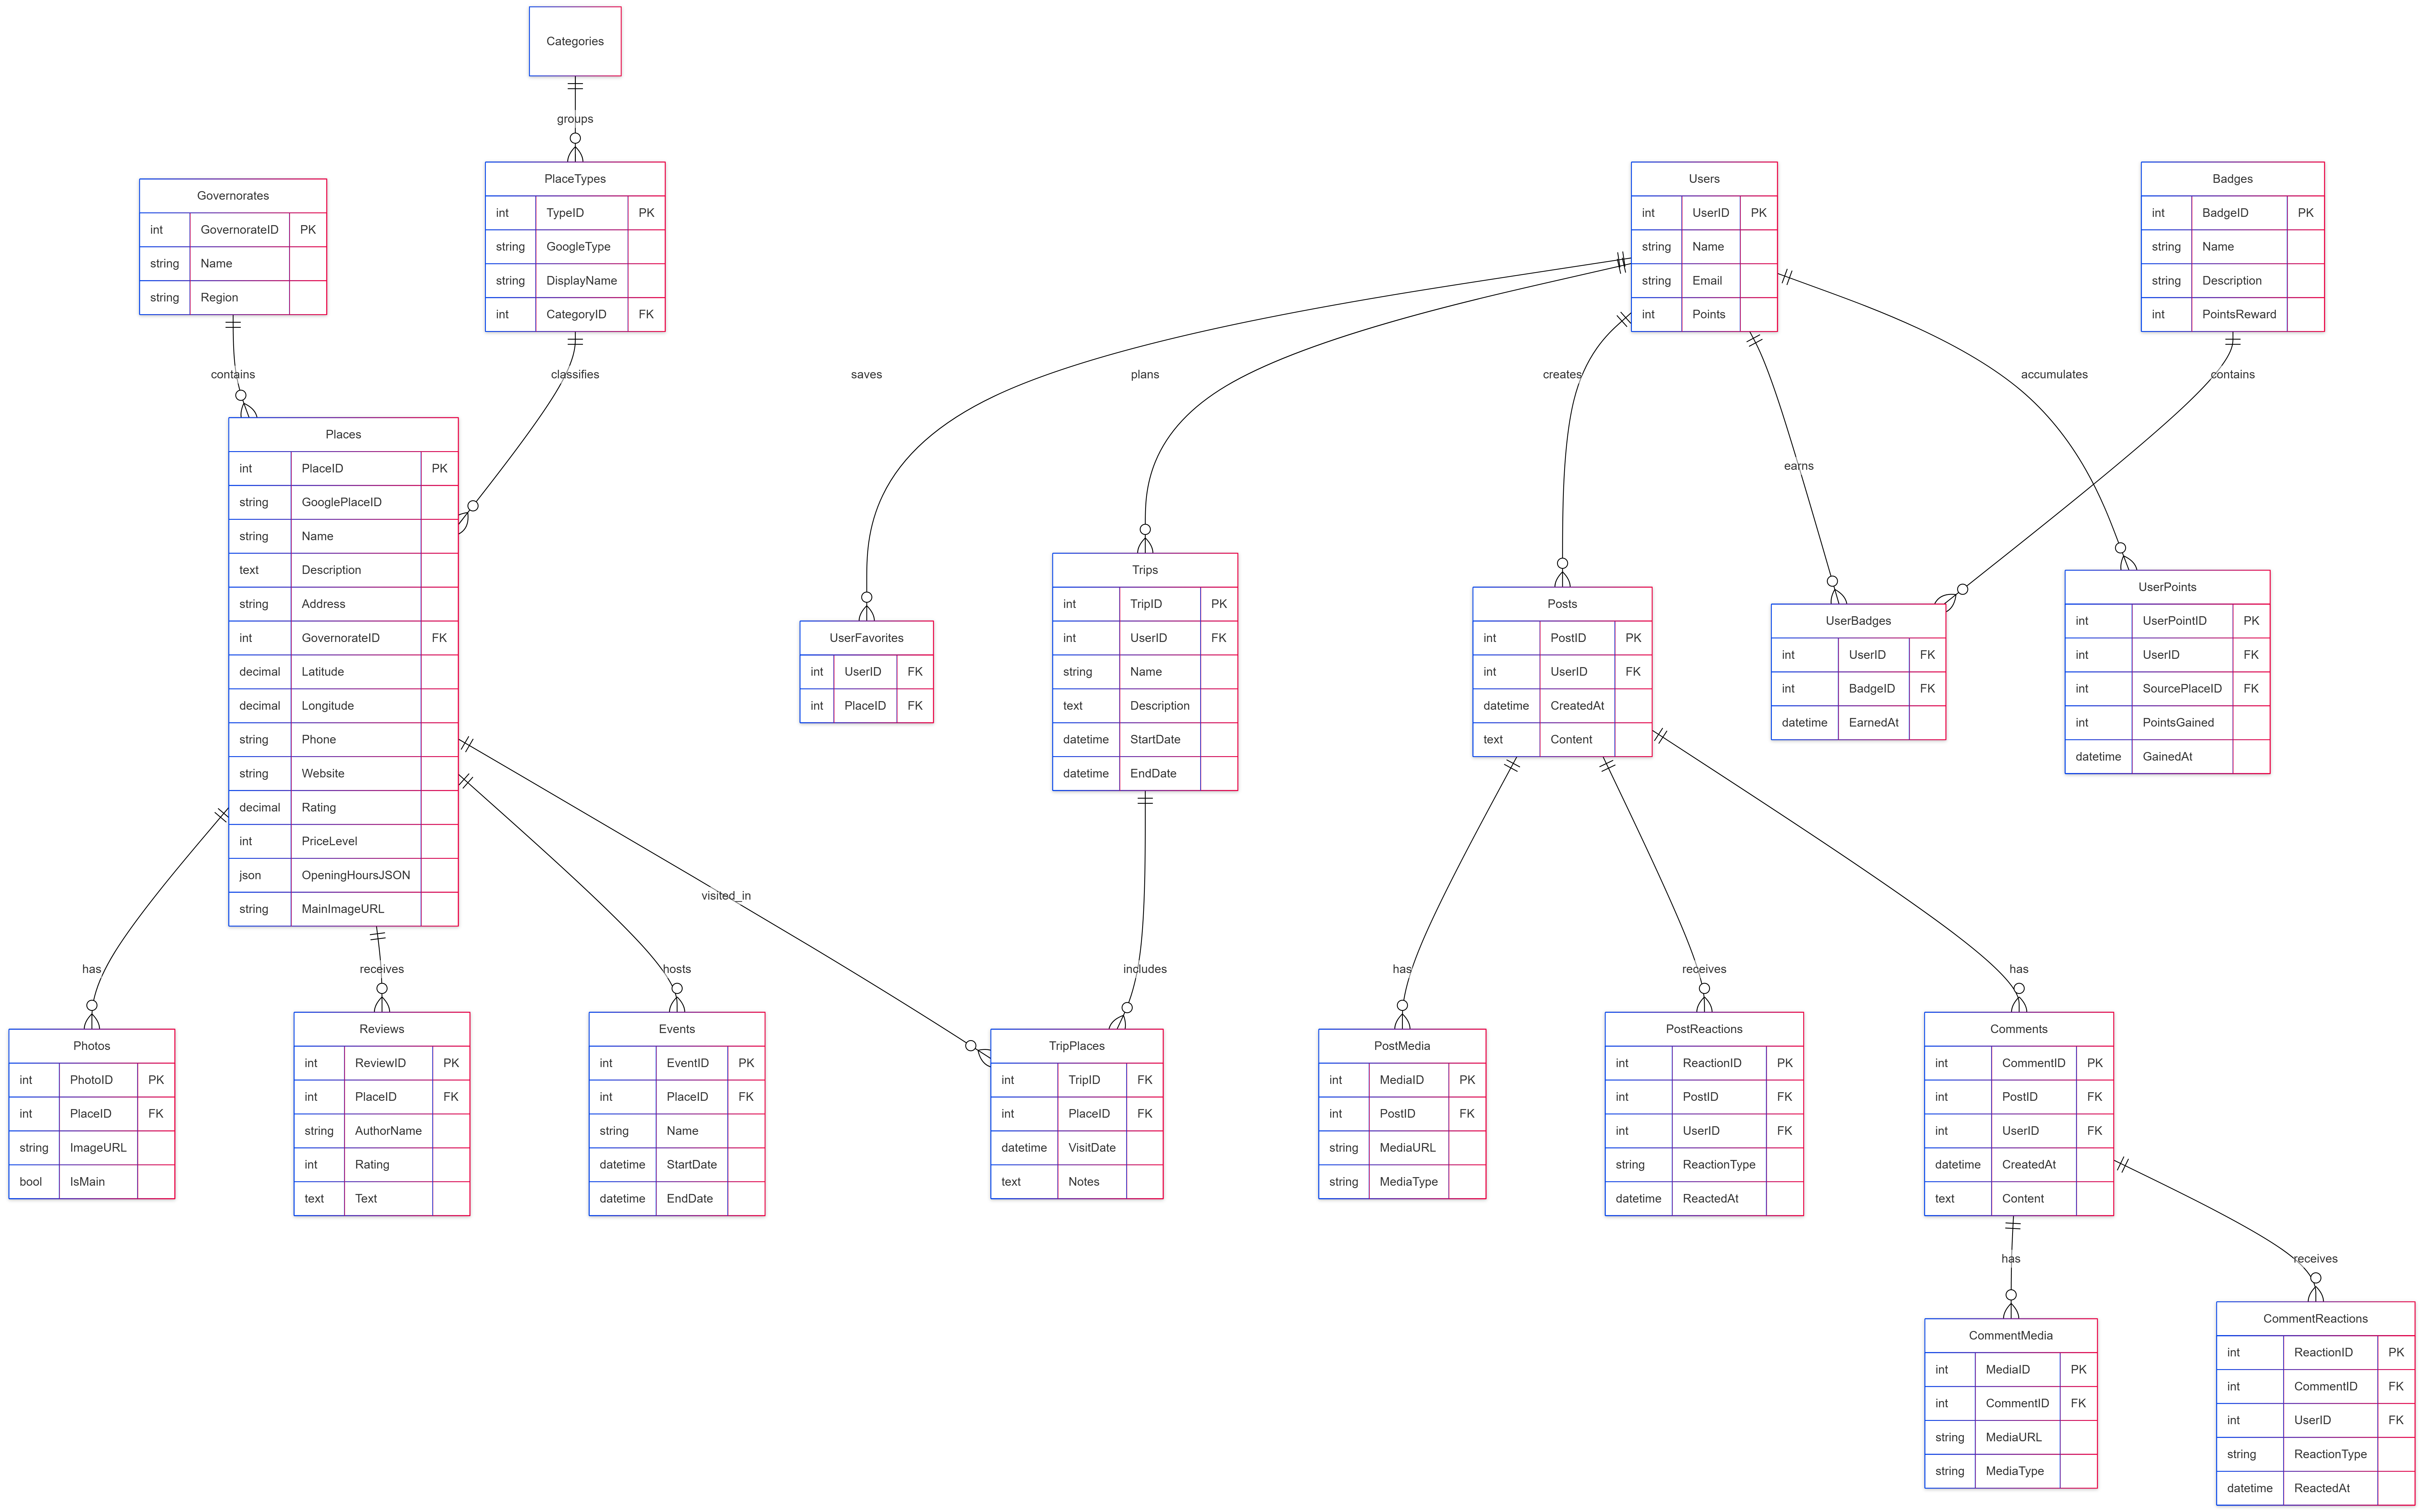
\includegraphics[width=\textwidth]{figures/erd.png}
    \caption{Kemora Full Database Entity Relationship Diagram}
    \label{fig:appendix_erd}
\end{figure}


\chapter*{Glossary and Abbreviations}
\addcontentsline{toc}{chapter}{Glossary and Abbreviations}

\begin{description}
    \item[API] Application Programming Interface. A set of rules that allows different software entities to communicate.
    \item[DTO] Data Transfer Object. An object that carries data between processes to reduce the number of method calls and network overhead.
    \item[EF Core] Entity Framework Core. An open-source, lightweight, and extensible object-relational mapper (O/RM) for the .NET ecosystem.
    \item[JWT] JSON Web Token. An open standard (RFC 7519) that defines a compact and self-contained way for securely transmitting information between parties as a JSON object.
    \item[LLM] Large Language Model. A deep learning algorithm, utilizing transformer architecture, that can recognize, summarize, translate, predict, and generate human-like text.
    \item[POI] Point of Interest. A specific geographical location (e.g., restaurant, museum, or landmark) that a user may find useful or interesting.
    \item[RAG] Retrieval-Augmented Generation. An AI architectural framework that retrieves data from external knowledge bases and injects it into an LLM's context window to ground the generation and prevent hallucinations.
    \item[SERP] Search Engine Results Page. The page displayed by a search engine in response to a query, previously utilized for targeted image fetching.
    \item[UI/UX] User Interface / User Experience. The graphical layout and the holistic interactive experience provided to the end-user by the application.
    \item[UUID] Universally Unique Identifier. A 128-bit label used for information in computer systems, heavily utilized as Primary Keys in the Kemora database.
\end{description}


\end{document}
